\documentclass{sysuthesis}
%这是中山大学本科毕业论文非官方模版0.0.4的一部分
%维护者为陈颂光(1m02math@126.com)
%任何人可以自由使用本文件
%然而,无法保证它完全符合学校的相关要求,甚至不保证它可以正常编译
%对于使用此模版造成的任何后果,维护者不负有任何责任

%论文题目应以简短、明确的词语恰当概括整个论文的核心内容,避免使用不常见的缩略词、缩写字。读者通过标题可大致了解毕业设计(论文)的内容、专业的特点和科学的范畴。中文题目一般不宜超过 24 个字,必要时可增加副标题。外文题目一般不宜超过 12 个实词。
\title{}%论文题目
\etitle{Spillover Effect of Sector Index: An explanation based on Input-Output Accounts}%英文论文题目
\author{李俊成}%作者
\authorx{李\ 俊\ 成}%封面上作者(各字符间可加空白)
\date{二〇一六年五月}%完成日期
\studentid{12335091}%学号
\school{数学与计算科学学院}%院(系)
\major{统计学}%专业
\mentor{刘京军(副教授)}%指导老师
%关键词是供检索用的主题词条(3—5 个),应采用能覆盖论文主要内容的通用技术词条(参照相应的技术术语标准)。按词条的外延层次排列(外延大的排在前面)。
\keywords{溢出效应;投入产出表;最小二乘回归}%中文关键词(每个关键词之间用“;”分开,最后一个关键词不打标点符号。)
\ekeywords{Spillover Effect; Input-Output Accounts; Least Square Regression}%英文关键词
\openingopinion{\rule{0cm}{6\baselineskip}}%开题报告中指导老师意见
\firstcheck{我阅读指导老师给的论文,选定投入产出表作为了研究的数据来源。写出了投入产出表研究相关的综述。目标是探索它在前沿学术期刊上如何被应用。}%第一次过程检查的学生总结
\firstopinion{\rule{0cm}{3\baselineskip}}%第一次过程检查的指导老师意见
\secondcheck{我明确了使用的数据,及分析的方法,尝试解释行业指数间的溢出现象。我使用编程解决了数据获取,清洗,分析等问题。}%第二次过程检查的学生总结
\secondopinion{\rule{0cm}{3\baselineskip}}%第二次过程检查的指导老师意见
\thirdcheck{我尝试使用最小二乘回归估计溢出程度。得到回归的参数估计前,对时间序列作平稳性检验。}%第三次过程检查的学生总结
\thirdopinion{\rule{0cm}{3\baselineskip}}%第三次过程检查的指导老师意见
\forthcheck{我补充完成论文的整体,对表格,图片,代码,以及引用作进一步的检查。对表述上概念不清晰,不连贯的部分作进一步的修改,以符合论文格式的要求。}%第四次过程检查的学生总结
\forthopinion{\rule{0cm}{3\baselineskip}}%第四次过程检查的指导老师意见
\overallopinion{\rule{0cm}{8\baselineskip}}%整体完成情况的指导老师意见
\instructorcomment{\rule{0cm}{6\baselineskip}}%指导教师评语
\instructorgrade{\rule{0cm}{2\baselineskip}}%指导教师给予的成绩评定
\majorcomment{\rule{0cm}{4\baselineskip}}%答辩小组或专业负责人意见
\majorgrade{\rule{0cm}{2\baselineskip}}%答辩小组或专业负责人给予的成绩评定
\schoolcomment{\rule{0cm}{3\baselineskip}}%院系负责人意见
\schoolgrade{\rule{0cm}{2\baselineskip}}%院系负责人给予的成绩评定
\openingrep{
%接下来是开题报告内容
\begin{enumerate}
\item{研究背景、目的:}
\begin{itemize}
  \item{影响一个行业相关股票价格的信息也影响关联行业的股价。即行业的股票价格的变化,存在对关联行业的溢出效应。这种溢出效应存在的基础是国民经济中,行业的生产活动是环环相扣,紧密相依的。本文的目的是利用投入产出表及证监会基于上司公司编制的行业指数,解释行业指数间的溢出效应。为认识风险及构建投资组合提供新的角度。}
\end{itemize}
\item{研究方法、步骤:}
\begin{itemize}
  \item{研究方法是实证分析,收集投入产出表及行业指数数据,分别找出每个行业指数中关联最密切的上游行业的行业指数和下游行业的行业指数,并根据投入产出表中行业关联的强度进行加权,为了刻画溢出溢出效应的强度,对其波动率时间序列进行回归。解释回归结果,探究行业的波动率多大程度上可以被上游行业和下游行业的波动率解释。}
\end{itemize}
\item{拟定进度安排}
\begin{itemize}
  \item{2016年3月4日:选题为:行业溢出效应基于投入产出表的解释,书写论文开题报告;}
  \item{2016年3月4日至2016年3月20日:查阅文献资料,收集论文所需的数据,对数据作筛选,清洗和处理;进一步查阅分析溢出效应的已有方法及相关文献资料;}
  \item{2016年3月21日至2016年3月31日:拟定论文初稿;}
  \item{2016年4月1日至2016年4月29日:根据指导老师反馈,对初稿论文中有问题的部分进行修改,获得定稿,同时对论文进行修改、复查。}  
\end{itemize}
\end{enumerate}
}
\cabstract{
本文以证监会行业分类下的行业指数为研究对象,利用2012年的中国投入产出表中行业相互关联的信息,对每个行业中的上游行业和下游行业进行了界定,挑选出关联最密切的行业,根据他们中间使用部分的流量进行加权。本文利用加权后的上游行业指数和下游行业指数共同解释上述行业指数对待研究的行业指数的溢出效应,并且以饲料行业所属的食品加工行业指数从2001年3月到2016年3月的数据作实证分析。结果表明,在两周的延滞以内,行业指数间溢出效应明显。即上游行业和下游行业在前一时间点的周对数收益率和周波动率分别解释本行业当前的周收益率和周波动率。这一发现表明,指数走势价格的信息,可以沿着行业相互依赖关系扩散。
}
\eabstract{This paper explains the spillover effect of sectoral indices created by CSRC. To further investigate the spillover effect, relations of supplier industries and customers industries are carefully investigated through the 2012 input output account of China. The results show that the yield and the volatility of supplier industry and customer industry in the previous week account for the spillover effect of yield and volatility of given sector respectively. Such finding indicates that information related to supplier and customer industries can affect the stock prices of given sector by diffusing gradually through the input output account.
}
\begin{document}
\frontmatter
\cleardoublepage
\tableofcontents%目录
\cleardoublepage
\listoftables%表格目录(不需要则可以把这两行去掉)
\cleardoublepage
\listoffigures%插图目录(不需要则可以把这两行去掉)
%\cleardoublepage
%\listofalgorithms%算法目录(不需要则可以把这两行去掉)

\mainmatter
%现在开始正文
\chapter{引言}
本章的主要目的是建立研究问题的背景,追问研究问题的意义,理清研究问题的思路。
\section{研究背景及问题}

影响一个行业相关股票价格的信息也影响关联行业的股价。即行业的股票价格的变化,存在对关联行业的溢出效应。例如,当生猪价格预期走高时,投资者根据这一利好消息,大量买入以养殖猪为主营业务的上市公司的股票,这些股票的价格快速上涨。但当其他投资者再进入市场时,这些股票的价格已经到达高位,此时再购买难以获利,对于新进入的投资者,还想要获利的方法是购买为猪养殖提供生产资料的上市公司的股票。例如,销售猪饲料或营养品为主营业务的上市公司,或为猪只提供育种服务的上司公司的股票。为何投资者会作出这样的推断?因为经济中各行业的生产活动是环环相扣,紧密相依的。溢出效应存在的基础是经济中投入和产出的关联。也就是说,溢出效应是经济中投入产出存在关联的一种表现,它是客观存在的。本文的目的是利用投入产出表,以及证监会基于上司公司编制的行业指数,以行业指数解释行业间的溢出效应。

溢出效应是资产配置及风险管理时必须考虑的重要问题。针对溢出现象,前沿的解释主要集中在两个方面,一方面是内在关联,例如,基本面上联系更密切的股票,走势上更可能同步。另一方面是传染现象,即稳健的企业的股价,因为市场中其他股票的走势急剧波动而关联到自身,自身也陷入急剧波动中。在股票市场建立的早期,传染现象是影响股价溢出效应的主要因素,投资者对信息的反应往往是过激的,结果是不同行业指数的收益率序列出现同涨同跌的情形。具体表现为,“政策市”成为了关注的热点。然而,随着我国股票市场逐渐完善和开放,研究的重点也逐渐转移到探究股票市场内不同行业对应上市公司之间的关联,对这种内在关联的把握和探究,为我们更好地理解投资者决策,提供了重要的基础。

内在关联探究的一个重要维度是经济体系中,行业间的投入和产出的关联。经济体系中,行业分工现象的普遍存在,例如,钢铁行业的产出,依赖于煤炭行业和矿石采选行业的产出。建筑行业的产出,依赖于钢铁行业的投入。行业链的存在表明行业间是相互依存的。这种依存关系最常用的刻画方式是投入产出表。投入产出表计算了在一个特定的时间段内,国民经济中各行业的活动的流量。基于行业间流量的高低,可以得到行业间关联的强度。投入产出表是经济活动一个更细致的快照。它为经济问题的研究,尤其是实证研究,提供了重要的依据。基于投入产出表的前沿研究主要集中在经济现象的解释。本文的研究问题为,资产价格波动的溢出现象,多大程度上可被行业投入和产出的关联信息解释。

\section{研究意义及思路}

\subsection{为什么用投入产出表解释溢出现象}

把握行业客观联系程度是解释股票市场中溢出现象的基础。基于投入产出表的信息,本文提出了两个假设,第一个,在同一个时间点内,若行业间的中间使用部分的产出的价值量或中间使用部分的投入的价值量越大,则行业间的客观联系越发紧密;第二个,我们可以根据该时间段内的投入产出表,推断附近的时间段中,行业间相关上市公司股票相互关联的程度,相互关联程度越高,股价的溢出现象越明显。
% 股价的溢出现象,可被实体经济联系及投资者的行为分别解释。一方面,对于实体经济中的每一个行业,与之密切关联的行业股价波动更可能同步,另一方面,投资者的决策,即他们对相关信息的反映,可以导致股价同步变动,Goldstein \cite{goldstein_contagion_2004-1}探究了同时投资两个资产的投资者,由于财富效应撤资,造成两个资产价格同向波动的问题。他强调,撤资行为可以在两个行业的不存在关联且一个行业受到冲击的情况下发生。
\subsection{为什么用行业指数观测溢出现象}

已有研究大多基于行业中具有代表性的个股,可见Hou\cite{kewei_hou_industry_2007},Ahern\cite{ahern2013network},Menzly\cite{menzly_market_2010}等人的研究,本文与已有研究的一个区别是,选用的观测对象是行业指数。选择行业指数是基于以下的理由:

行业指数最能代表实体经济行业的活动变化。证监会行业指数中覆盖的上市公司,业务收入的50\%或其业务利润的30\%归属其所在的行业,若两个标准都没有达到,则由上市公司行业分类专家组成的委员会根据公司实际经营状况,判断公司行业归属;归属不明确的,划为综合类\cite{_2012_????}。这个分类标准一定程度上克服了多元化经营的上市公司分类不清晰的问题。

行业指数的数据可得性好,与季度发布甚至年度发布一次的财务报表数据相比,行业指数的数据随交易日同步更新。而且,行业指数中包含的往往是一揽子的上司公司,与个股相比,行业指数避免了个股由于重大信息公布导致的停牌,既而数据点有缺失的问题。

股票市场中信息能够充分流动,并在较短时间内反映在股价的变化上。虽然上市公司组成的行业指数并不一定充分代表整个行业的全体,具体表现为,一些行业指数中上市公司的市值之和远小于它在投入产出表中的流量。但是,这一问题可被减缓。我们在选取样本时,汇总各个行业指数中与之关联的关键行业,得到一个面板数据,将这个面板数据作为评估的样本全体。

\subsection{研究思路}

研究思路主要分为三部分,第一部分是背景资料的搜集,第二部分数据的处理,第三部分是数据的分析和解读。每一部分的思路都是从问题背景开始,到定位问题,再到寻找原因,最后到寻找解决方法。

第一部分的问题背景是行业板块间的联动现象客观存在,进一步地,本文希望定位出这种联动现象客观存在的原因是什么,原因是实体经济当中存在客观的联系,经济生产活动以提高效率为目标,围绕着产品的生产,进行分工。既而出现了行业,而笔者可得的数据中,最细致地刻画行业间相互依存的关系的是投入产出表。因此,使用投入产出表,刻画行业间的生产活动的依赖关系,投入产出表的表式可见图\ref{fig:ioaccount}及图\ref{fig:ioaccount-quardone}。

第二部分的问题是,如何分析这种依赖关系在实际中的影响。由于投入产出表基表编制的时间长,数据样本有限。因此,第二部分的问题是如何增加可以研究的数据样本。股票市场中数据样本充足,因此,我们比较了取行业个股和取行业指数的两种方法,最后确定行业指数为研究对象。本文尝试从行业指数中指数价格的变动,找到溢出效应存在的线索。然而,要以什么样的方式,建立投入产出表和行业指数间的对应关系,才能使得一个行业的上司公司充分代表所在的行业,已有的研究没有给出方法。为此,本文寻找并比较了多种行业指数编制的标准,最终挑选出证监会的指数分类标准,节选的分类标准可见图\ref{fig:classify-output},并且以该指数为标准,花费了大量的精力和时间,建立起了行业指数和行业投入产出在所属行业和流量上的对应关系,节选部分参考图\ref{fig:iomapping},得到了重新编制后的基于行业指数的流量矩阵,结果可见图\ref{fig:reorganized-ioaccount}。除此以外,由于指数编制过程中,指数的基点和基期不一,为了克服尺度上的差异,考虑研究指数的对数收益率(下文简称收益率)及波动率,进一步地,还需要考虑时间尺度上的问题,数据的频次有日内,日,周,月,季度,年等,对于本文的研究问题而言,周序列是较好的尺度,它是噪音与信号的一个较好的平衡,本文中的噪音指投资者因为非行业间关联而进行的投资操作,例如“超短线”操作,以及由于节假日的存在,使得每日交易信息中所包含的信息量不对称,例如“周末效应”或“节假日效应”。而信号是行业间关联的信息,扩散到行业的过程。为了降低噪音以提取信息,本文提出了几个具有创造性的处理方法。

第三部分是探究行业间收益率如何相互影响及行业间波动率如何相互影响,这需要考虑如何结合投入产出表中的信息。对于待研究的行业而言,要同时考虑上游行业和下游行业的影响,但影响的强度又由于行业间连接强度不同而有所差别。为了刻画这种差别,将投入产出表中的流量作为权重,对上游行业和下游行业分别作加权,得到新的指数收益率和波动率。引入最小二乘回归模型解释变量间的动态相关关系。最小二乘回归有效的原因在于,待研究指数本身的信息,可以分解为被行业板块关联的线性组合的部分以及不可被行业板块间关联所解释的残差部分,而这种投影运算又和最小化残差部分的优化问题结果是相同的。如果溢出效应确实存在,那么,从统计的角度来看,关联行业板块的系数估计应是显著的。同时,为了避免伪回归问题,即两个序列仅仅因为在时间上的排列顺序是从后往前的,回归发现估计系数即显著的问题,在使用最小二乘回归模型前,先对收益率序列作平稳性检验。

  \begin{figure}[h!tbp]
  \centering
  
\includegraphics[scale=0.65]{image/投入产出表_1.png}
  \caption{投入产出基表表式(图示)}
  \caption*{\footnotesize 第\uppercase\expandafter{\romannumeral1}
象限是本文数据采集的对象。投入产出表第\uppercase\expandafter{\romannumeral1}
象限是中间投入的部分,主栏对应中间投入,宾栏对应中间使用。中间投入部分是一个$n \times n$的方阵,$n$是当年投入产出表中行业的总数。第i行为第i个行业在统计时间段内对各个行业的产出量。第j列是第j个行业在统计时间段内依赖各个行业的投入量。第\uppercase\expandafter{\romannumeral2}
象限是第I象限在水平方向上的延伸,主栏的部门分组与第\uppercase\expandafter{\romannumeral1}
象限相同;宾栏由最终消费、资本形成总额、出口等最终使用项目构成。 沿着行的方向上看,刻画某行业生产的货物或服务使用在各种最终使用途径的当期价值量;沿列方向看,刻画各种最终使用的规模及其组成。第\uppercase\expandafter{\romannumeral1}
象限和第\uppercase\expandafter{\romannumeral2}
象限共同组成了一个横表,反映国民经济中,各行业生产的货物或服务的使用去向,即各行业的中间使用以及最终使用的数量。第\uppercase\expandafter{\romannumeral3}
象限是第\uppercase\expandafter{\romannumeral1}象限在垂直方向的延伸,主栏由劳动者报酬、生产税净额、固定资产折旧、营业盈余等各种增加值项目组成;宾栏的部门分组与第\uppercase\expandafter{\romannumeral1}
象限相同。 而第\uppercase\expandafter{\romannumeral3}象限刻画的是经济中每个行业增加值及其组成成分。第\uppercase\expandafter{\romannumeral1}
象限和第\uppercase\expandafter{\romannumeral3}
象限连接组成的竖表,反映国民经济中,各个行业在经营以及生产活动中的各项投入的来源及产品的价值组成,即各个行业的投入总量以及其所包含的中间投入和增加值的数量。投入产出表的三大象限相互连接,从总量上,以及结构上全面又系统地反映国民经济各部门从生产到最终使用这一完整的实物运动过程中的相互联系。 }
  \label{fig:ioaccount}
  \end{figure}

  \begin{figure}[htbp]
  \centering
  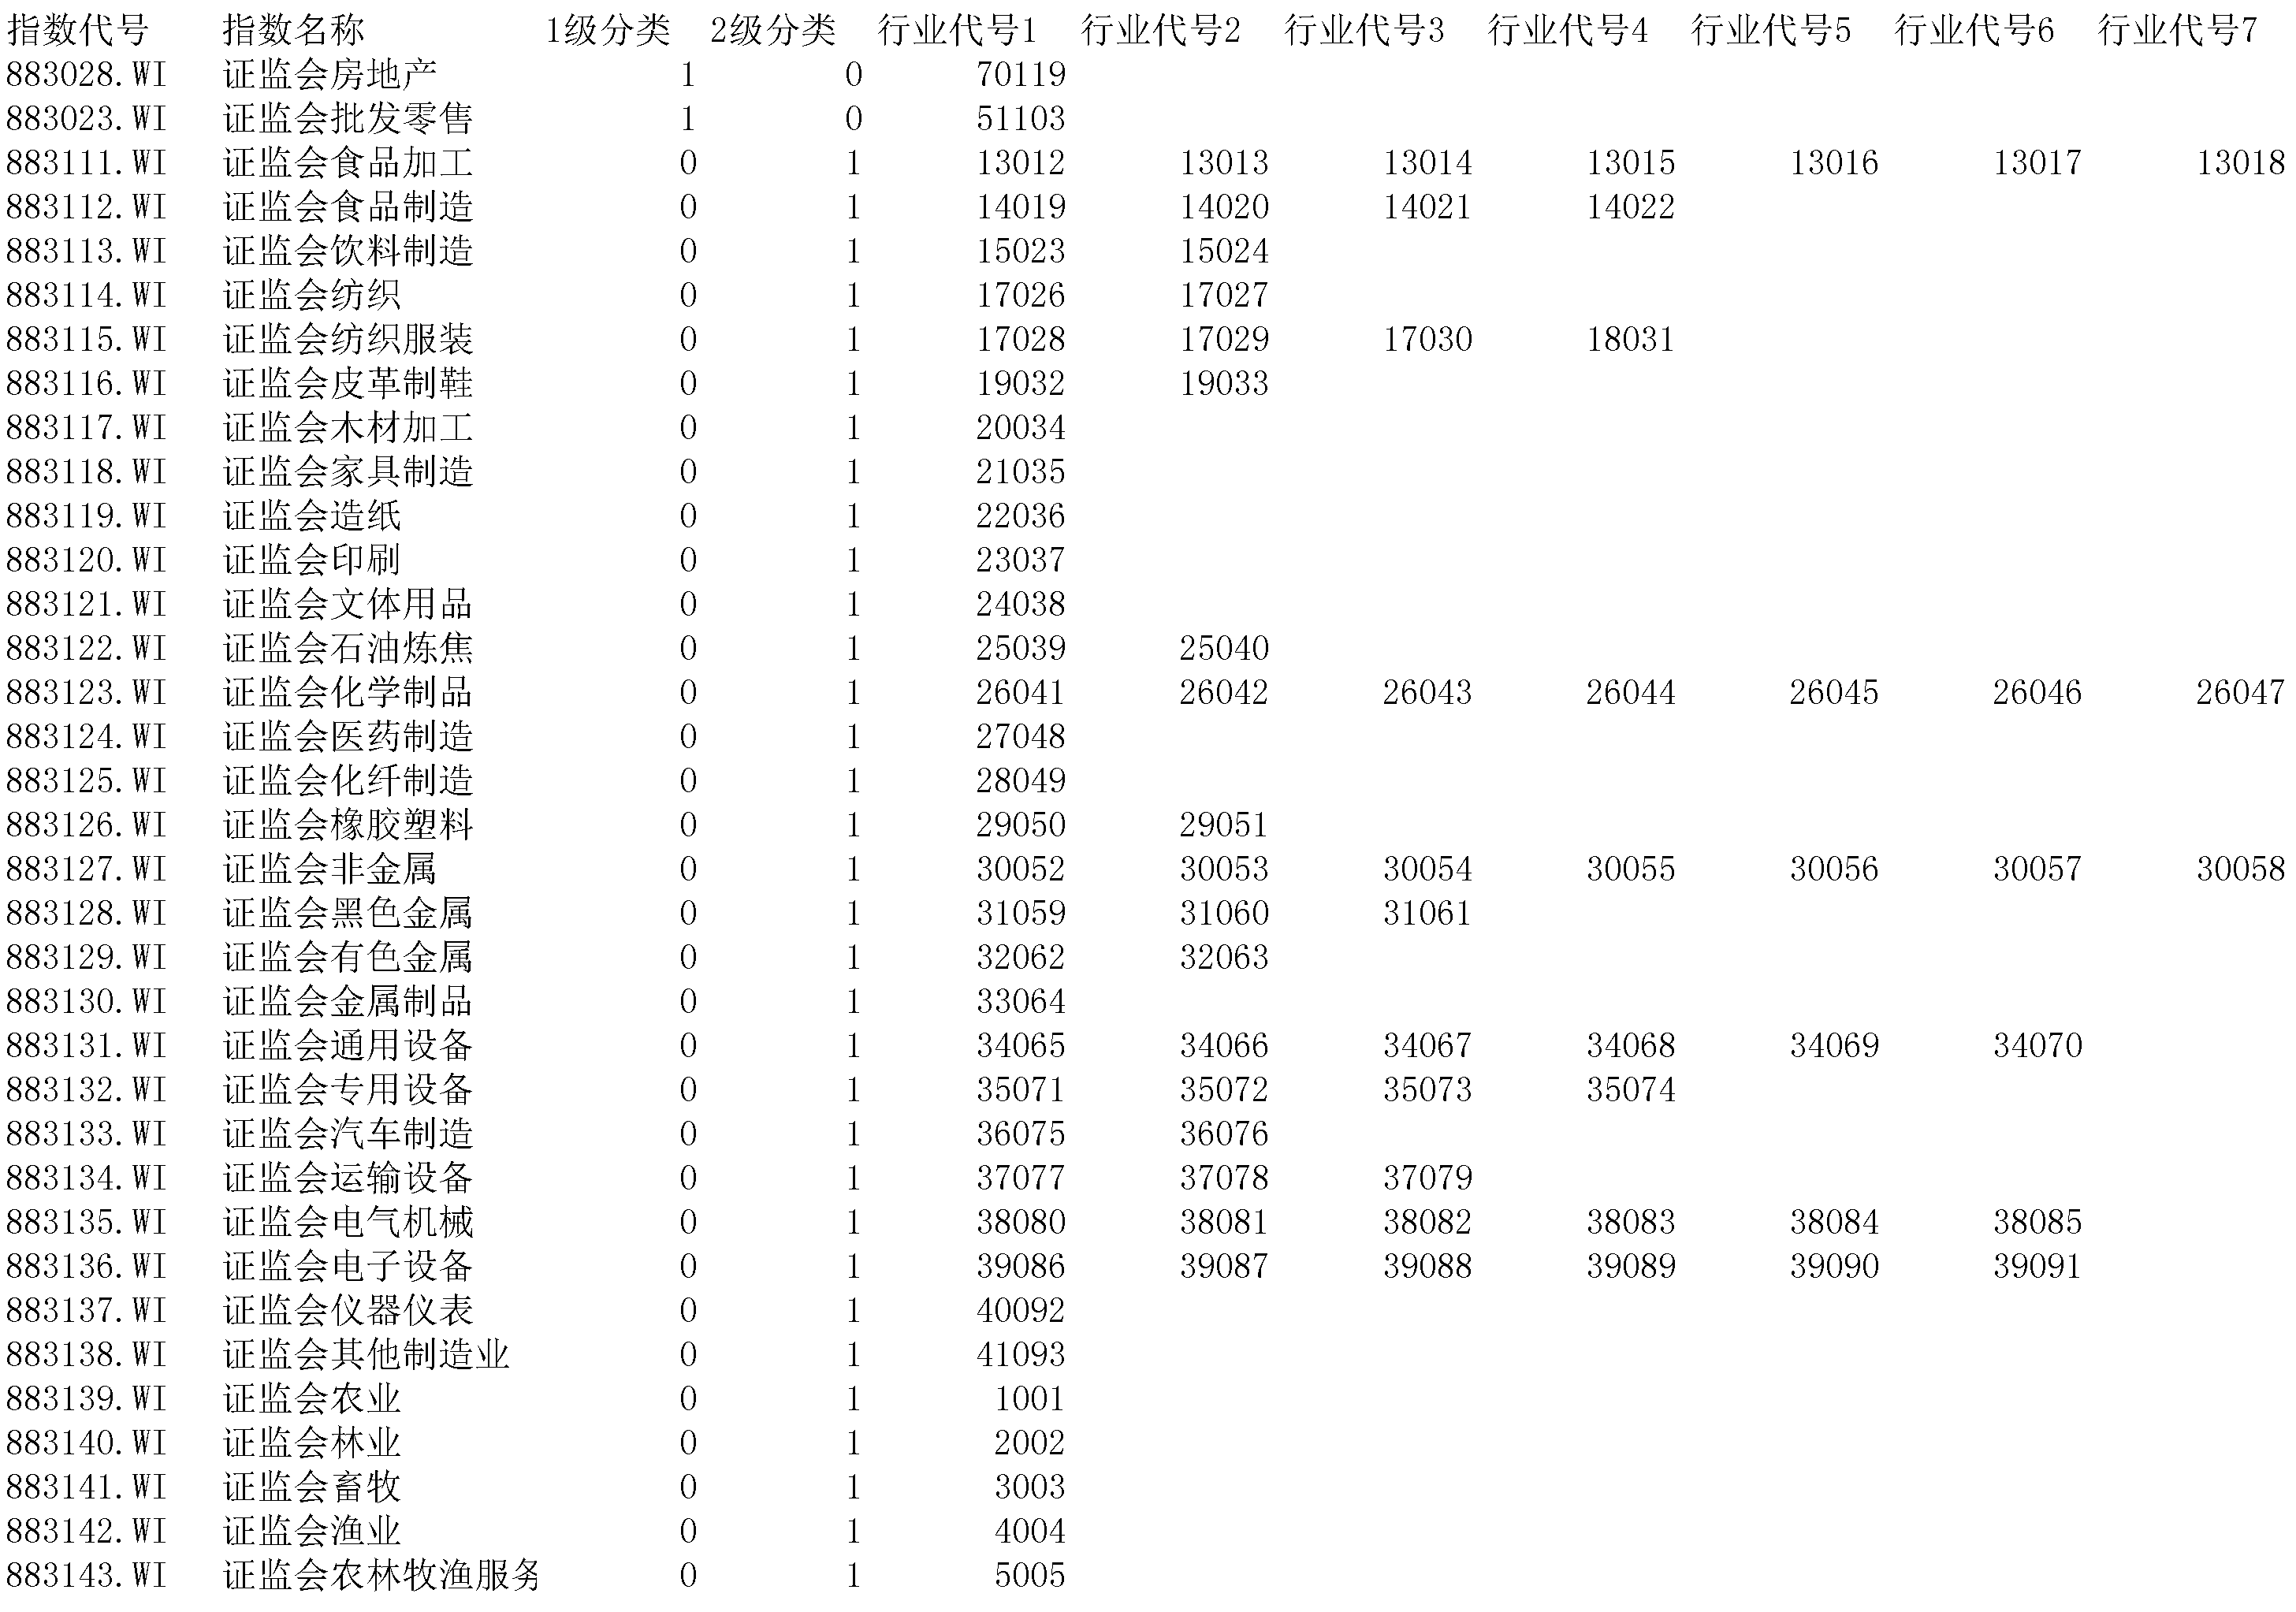
\includegraphics[scale=0.65]{image/行业与指数对应关系.png}
  \caption{上市公司行业指数及投入产出表行业的对应关系(节选图)}
  \caption*{\footnotesize 对应关系表的第一栏是行业指数在WIND资讯金融终端的代号;第二栏是该行业指数的名称;第三栏是一个逻辑标记,判断该行业是否为一级行业,如果为一级行业,那么标记为1,否则标记为0;第四栏也是一个逻辑标记,判断该行业是否为二级行业,如果为二级行业,那么标记为1,否则标记为0;第五栏到第十一栏是纳入该指数的行业在投入产出基表中的代号,分类标准主要基于上市公司行业分类指引在2015年第四季度更新的报表\cite{_20154._SEC_Categorize}。该报表中,上市公司的行业分类代号中的第二列的行业大类代码与投入产出基表中的代码前两位含义相同。}
  \label{fig:iomapping}
  \end{figure}

\subsection{可能的创新}

本文选择的观测对象是行业指数。已有的研究的观察,往往选取行业中具有代表性的个股为研究对象,但本文采取的是行业指数为研究对象。与个股相比,行业对象更能够反映经济网络中,行业中的投入-产出关联。

本文为行业指数溢出现象提供更有实际背景的解释。行业之间相关联的程度,若以指数走势的相关系数来估计,具有估计不稳定,且缺乏解释力的问题。本文基于收益率尝试为这种关联提供基于经济基本面数据的解释,协助投资者更好地评估风险。

\subsection{本文重要结论}

溢出效应在行业指数中普遍存在。具体表现为,待研究的行业的在该时间点的收益率以及波动率,很大程度分别被相关的上游行业的行业指数及下游行业的行业指数在前一周的收益率和波动率所解释。这一现象表明,影响股价的信号,可以沿着产业链,从上游产业对应的上市公司及下游产业对应的上市公司传导到待研究的行业。这一现象在指定行业后,并不随着关联行业的数目的改变而有显著的变化。

\subsection{本文研究框架}

本文余下分为几部分:第二章为综述;第三章为数据采集和处理;第四章分析溢出效应,叙述该效应存在基于的假设,探究的方法,以及分析结果;第五章为结束语。

\chapter{综述}
本章的目的是发掘前沿研究文献中的问题,理清相关文献的思路,探索可以进一步研究的空间。
\section{溢出效应相关综述}

溢出效应的存在,是真实的股票市场中存在交易的摩擦以及信息的不对称的推论。这一推断来自于Hong等人\cite{hong_industries_2002}提出的观点。一个指数在给定时间点的价格,不一定充分纳入该时间点前影响价格的信息。这一发现为后续的相关研究开拓很大的空间,即哪些信息或指标对股价产生了影响,这种影响扩散的速度有多快。Hou\cite{kewei_hou_industry_2007}探究了属于同一行业的美国上市公司股价的收益率序列,对不同类型的信息,例如,成交量及竞争企业的盈利表现,表现出的溢出效应。但是,他的研究没有解释行业间的信息流动的溢出关系对收益率序列的影响。后续的研究对此作了补充。Menzly\cite{menzly_market_2010}发现,对于美国投入产出表中,较为重要的几个产业对应的上市公司从1960年到2009年的收益率序列作领先-延滞现象的检测,发现信息可以沿着供应链传导到股票价格,即信息传导受行业间在投入产出网络上的关联程度影响。

溢出效应的另一种解释是传染现象。即经济中正常运作的个体,由于受到其他行业或企业的经营状况不佳的影响,既而自身也受到波及的情形。具体表现为,在危机期间,经济个体间的相关性急剧上升。传染效应的前沿研究主要集中在欧元区债务危机期间。主要的研究目的是借助定量分析的结果,来为债务危机发生的原因作一个定性分析,具体地说,即争论是由于内在关联的日切紧密,导致了传染更容易,还是说只是因为投资者的过度反应,导致了传染现象的发生。这一争论的源头是来自于Forbes和Rigobon等人认为,历史的金融危机,例如1997年的亚洲金融风暴,不是由于投资者过度反应所导致的传染现象导致的,而是由于他们内在关联日益紧密,具体地说,即危机前资产间的相关性已经在上升,而危机阶段将剧烈地波动的影响纳入考量后,这种相关性并没有因为危机期间而上升到异常高的情形。\cite{forbes_no_2002-1},然而,后续在欧元债务区危机的研究当中,Arghyrou\cite{arghyrou_emu_2012}及Smimou等研究者发现\cite{smimou_intensity_2015},投资者的期望的偏移,对危机的持续发酵,即传染持续存在起了关键的作用。本文认为,传染现象领域的研究最大的启发在于,传染效应集中爆发的基础是危机的发生,但是,危机持续的时间与实体经济周期中平稳或增长的周期相比,是短暂的,从长期来看,行业和企业间的内在关联,更能够为传染现象的解释,提供更有解释力的信息。

\section{投入产出表相关综述}

投入产出表的前沿研究,主要集中在微观层次上,即单个行业的冲击与宏观层次上,即行业间的冲击之间的联系。Lucas\cite{lucas_understanding_1977}认为,随着行业数量增加,它在整体经济中的分量趋小。因此,一个行业的波动,对其他行业的冲击有限。也就是说,一个行业的波动更难影响整体的波动。然而,Acemoglu\cite{acemoglu_network_2012}对此提出了质疑。他认为,行业关联的方式,会极大地影响冲击的消散,既而小的波动会堆叠在一起,表现为宏观层面上显著的波动。他采用20世纪70年代以来美国的投入产出数据,进行了实证分析。它发现行业关联结构的变化,表现为行业间投入产出比例不对称的趋势加剧,明显减缓冲击传导的速度,结果是微小的波动叠加,对宏观经济形成更大的波动。波动速率取决于经济体系网络结构的变化,没有办法刻画行业的冲击随时间如何扩散。这为后续的研究留下了一片空间,即网络间每个行业的变动,多大程度上,受其上游行业和下游行业的情况的变动的影响。

Acemoglu\cite{acemoglu_microeconomic_2015}对于网络结构的研究为后续的研究指明了一个新的方向。他探究的重点是整个投入产出表中,不同行业间流量的差别,对于网络中冲击传导速度的影响。具体表现为,行业间流量的标准差越大,行业的冲击传导越缓慢。但他没有研究,细分到一个行业中,与其他行业关联之间,可以如何传导,而这一问题比起宏观的波动更值得研究。若以投入产出表中的行业为节点,流量为边的权重,这一网络,可以用图论的方式进行研究。因此,在他的研究基础上,许多研究者尝试结合图论中的一些信息,去定位哪些行业在投入产出表当中,最值得留意,图论中的信息,Opsahl\cite{opsahl_node_2010}的研究发现,这些信息包括但不限于,带权的入度和出度,介数中心度,特征中心度,聚类系数等。Ahern\cite{ahern2013network}利用图论中介数中心度,定位了美国的投入产出表最容易受到多次冲击的板块,他认为,一个行业越容易受到冲击,那么,它要承受更大的波动,具体地说,即这种波动对应的风险,应当有相应的溢价。因此,他在Fama-French\cite{fama_multifactor_1996}选股模型的基础上,引入中心行业及边缘行业超额收益率的差值,对超额收益率作进一步的解释。带权的路的研究,还可以用于行业冲击的路径的传导,Ahern\cite{ahern_importance_2014}试着通过Dyjkstra最短路算法,找出网络中每个行业受到冲击时,最先受到波及的其他行业。针对网络结构的研究已有的研究大多仍集中在个股的超额收益率的解释中,这一方向被Harvey等人最近提出的观点所质疑,即\cite{harvey__2016}过多的因子模型的解释力很弱,关联往往是伪回归。因此,本文尝试通过改变研究对象的方式,用行业指数,从而不依赖于与个股相关的一些变量,例如说市值,交易量等,来摆脱这一研究方法的局限性。

\chapter{数据获取与处理}
本章的目的是叙述数据的来源,数据清洗的方法。另外,本章中提及的表格都较为庞大,少则数十列,多则数百行,论文既有的版式无法将它们完整地展示。为了兼顾直观地展示处理方法及叙述最重要的思路,这些表格大多以节选图的方式进行展示,同时,附上适量的注释以详尽地说明表格中各栏目的作用。

\section{数据来源}
数据的来源有:国家统计局发布的《中国统计年鉴》的投入产出表,国民经济行业分类(GB/T 4754-2011)以及WIND资讯金融终端。本节的其余部分叙述各个数据的来源,对数据的内容作详尽的说明。
\begin{enumerate}
	\item {投入产出表}\\
	投入产出表描述了在给定的时间区域内,一国的经济中各行业的投入来源和产出去向,揭示了各部门间的依存关系\cite{_2002_????}。本文采用的投入产出表是投入产出基本表。它取自中国国家统计局编制的《中国国民经济核算体系》。本文选取的投入产出表基本表(下文简称:投入产出基表。)是2002年,2007年及2012年的投入产出基表。选用这三个时间点的投入产出表出于三个理由。第一,国家统计局每逢尾数为2和7的年份,会重新编制投入产出表基表;第二,投入产出基表对行业的刻画更为细致;第三,这三个时间点的跨度涵盖了大部分的行业指数上市时间段的走势。投入产出基表由三部分组成,称为第I、II、III象限,本文取第I象限,即投入产出表的中间投入部分探究行业间的关联。投入产出基表的表式如图\ref{fig:ioaccount}所示。将第I象限作一个更细致的观测,如图\ref{fig:ioaccount-quardone}所示。

  \item {上市公司分类标准}\\
  行业分类标准基于国民经济行业分类(GB/T 4754-2011)。2012年的中国投入产出表是按照该标准进行编制。同时,中国证监局\cite{_wind_????}对A股上市公司,分别按照该分类的一级行业标准及二级行业标准进行分类。其中,二级行业标准对一级行业标准进行细分,它对经济活动的刻画更加细致,也更有代表性,因此我们主要以二级行业分类标准下覆盖的经济行业为研究对象。分类结果的节选见图\ref{fig:classify-output}。

	\item {行业指数}\\
	行业指数通过WIND资讯终端采集。指数的权重由流通股本计算。采集数据的区间是从指数编制开始(2001年4月1日)到2016年3月1日。采集数据项目是月收益率及每月市值变化。由于国民经济行业分类标准在2011年作了修订,新增的行业指数的数据则从指数建立日算起。
\end{enumerate}

\section{数据处理}

数据处理过程分为两步。第一步:挑选上市公司行业分类标准及标的指数,力求分类标准最能反映投入产出表中行业的相互依存的关系。第二步:获取上市公司行业指数与投入产出表中行业的对应关系表;第三步:建立基于行业指数的中间投入矩阵。该投入矩阵一定程度上可反映行业指数间相互关联的强度。为了更直观地展示转化的流程,以及结果,引入转换时部分表格的节选图。

\subsection{挑选标的资产}

挑选的标的资产应尽可能贴近投入产出表中各行业之间的经济关联。已有的研究选取的是某个行业中具有代表性的个股,本文和已有研究的区别在于选取的标的资产是行业指数。在研究溢出效应时,行业指数优与行业个股相比,具有以下优势。首先,行业指数比行业个股更能代表行业整体的变化,行业指数的编制基于多家上市公司的股价,这些上市公司均以该行业经营活动为主要收入来源。其次,行业指数比行业个股流动性更好。个股在重大信息披露的时期往往停止股票交易,减少了可以采纳的样本。然而囊括多家同行业上司公司的行业指数,不受上述因素影响。

WIND资讯金融终端中,基于不同的分类标准,有不同的行业指数。本文挑选的是证监会行业指数。证监会行业指数与其他行业指数相比,有以下优势。首先,证监会行业指数中覆盖的上市公司,业务收入的50\%或其业务利润的30\%归属其所在的行业,若两个标准都没有达到,则由上市公司行业分类专家组成的委员会根据公司实际经营状况,判断公司行业归属;归属不明确的,划为综合类\cite{_2012_????}。这个分类标准一定程度上克服了多元化经营的上市公司分类不清晰的问题。其次,证监会编制的上市公司行业分类代号中的第二列的行业大类代码与投入产出基表中的代码前两位含义相同。这一点为行业指数和投入产出表建立对应关系提供了极大的便利。

\subsection {建立标的资产与投入产出表的对应关系}

证监会的上市公司行业分类与投入产出表的分类存在一些差异,这些差异主要体现在三个方面。一:一部分的行业在证券市场中没有上市公司,例如公益服务业,政府机构。二:有一部分的行业指数,一个指数包含多个子行业。三:由于行业分类标准在2011年发生了变动,因此,2007年及2002年的投入产出表中,有一部分指数对应的行业在表格建立的时候,没有细分。为了克服差异造成统计上的不便,我们额外制作了三个表格,每个表格都建立了当年投入产出表中各行业与证监会行业指数的对应关系。接着,我们按照表\ref{fig:iomapping},将投入产出表各行业中的流量,转化为各行业指数对应实体经济的流量,即表\ref{fig:reorganized-ioaccount}。  

建立了联系以后,可以将投入产出表中各行业之间相互依存的关系,用他们对应的行业指数来刻画。这种刻画是成立的,因为关联更密切的行业,行业指数的关联也更密切。基于行业指数的中间投入流量矩阵见图\ref{fig:reorganized-ioaccount}。

  \begin{figure}[h!tbp]
  \centering
  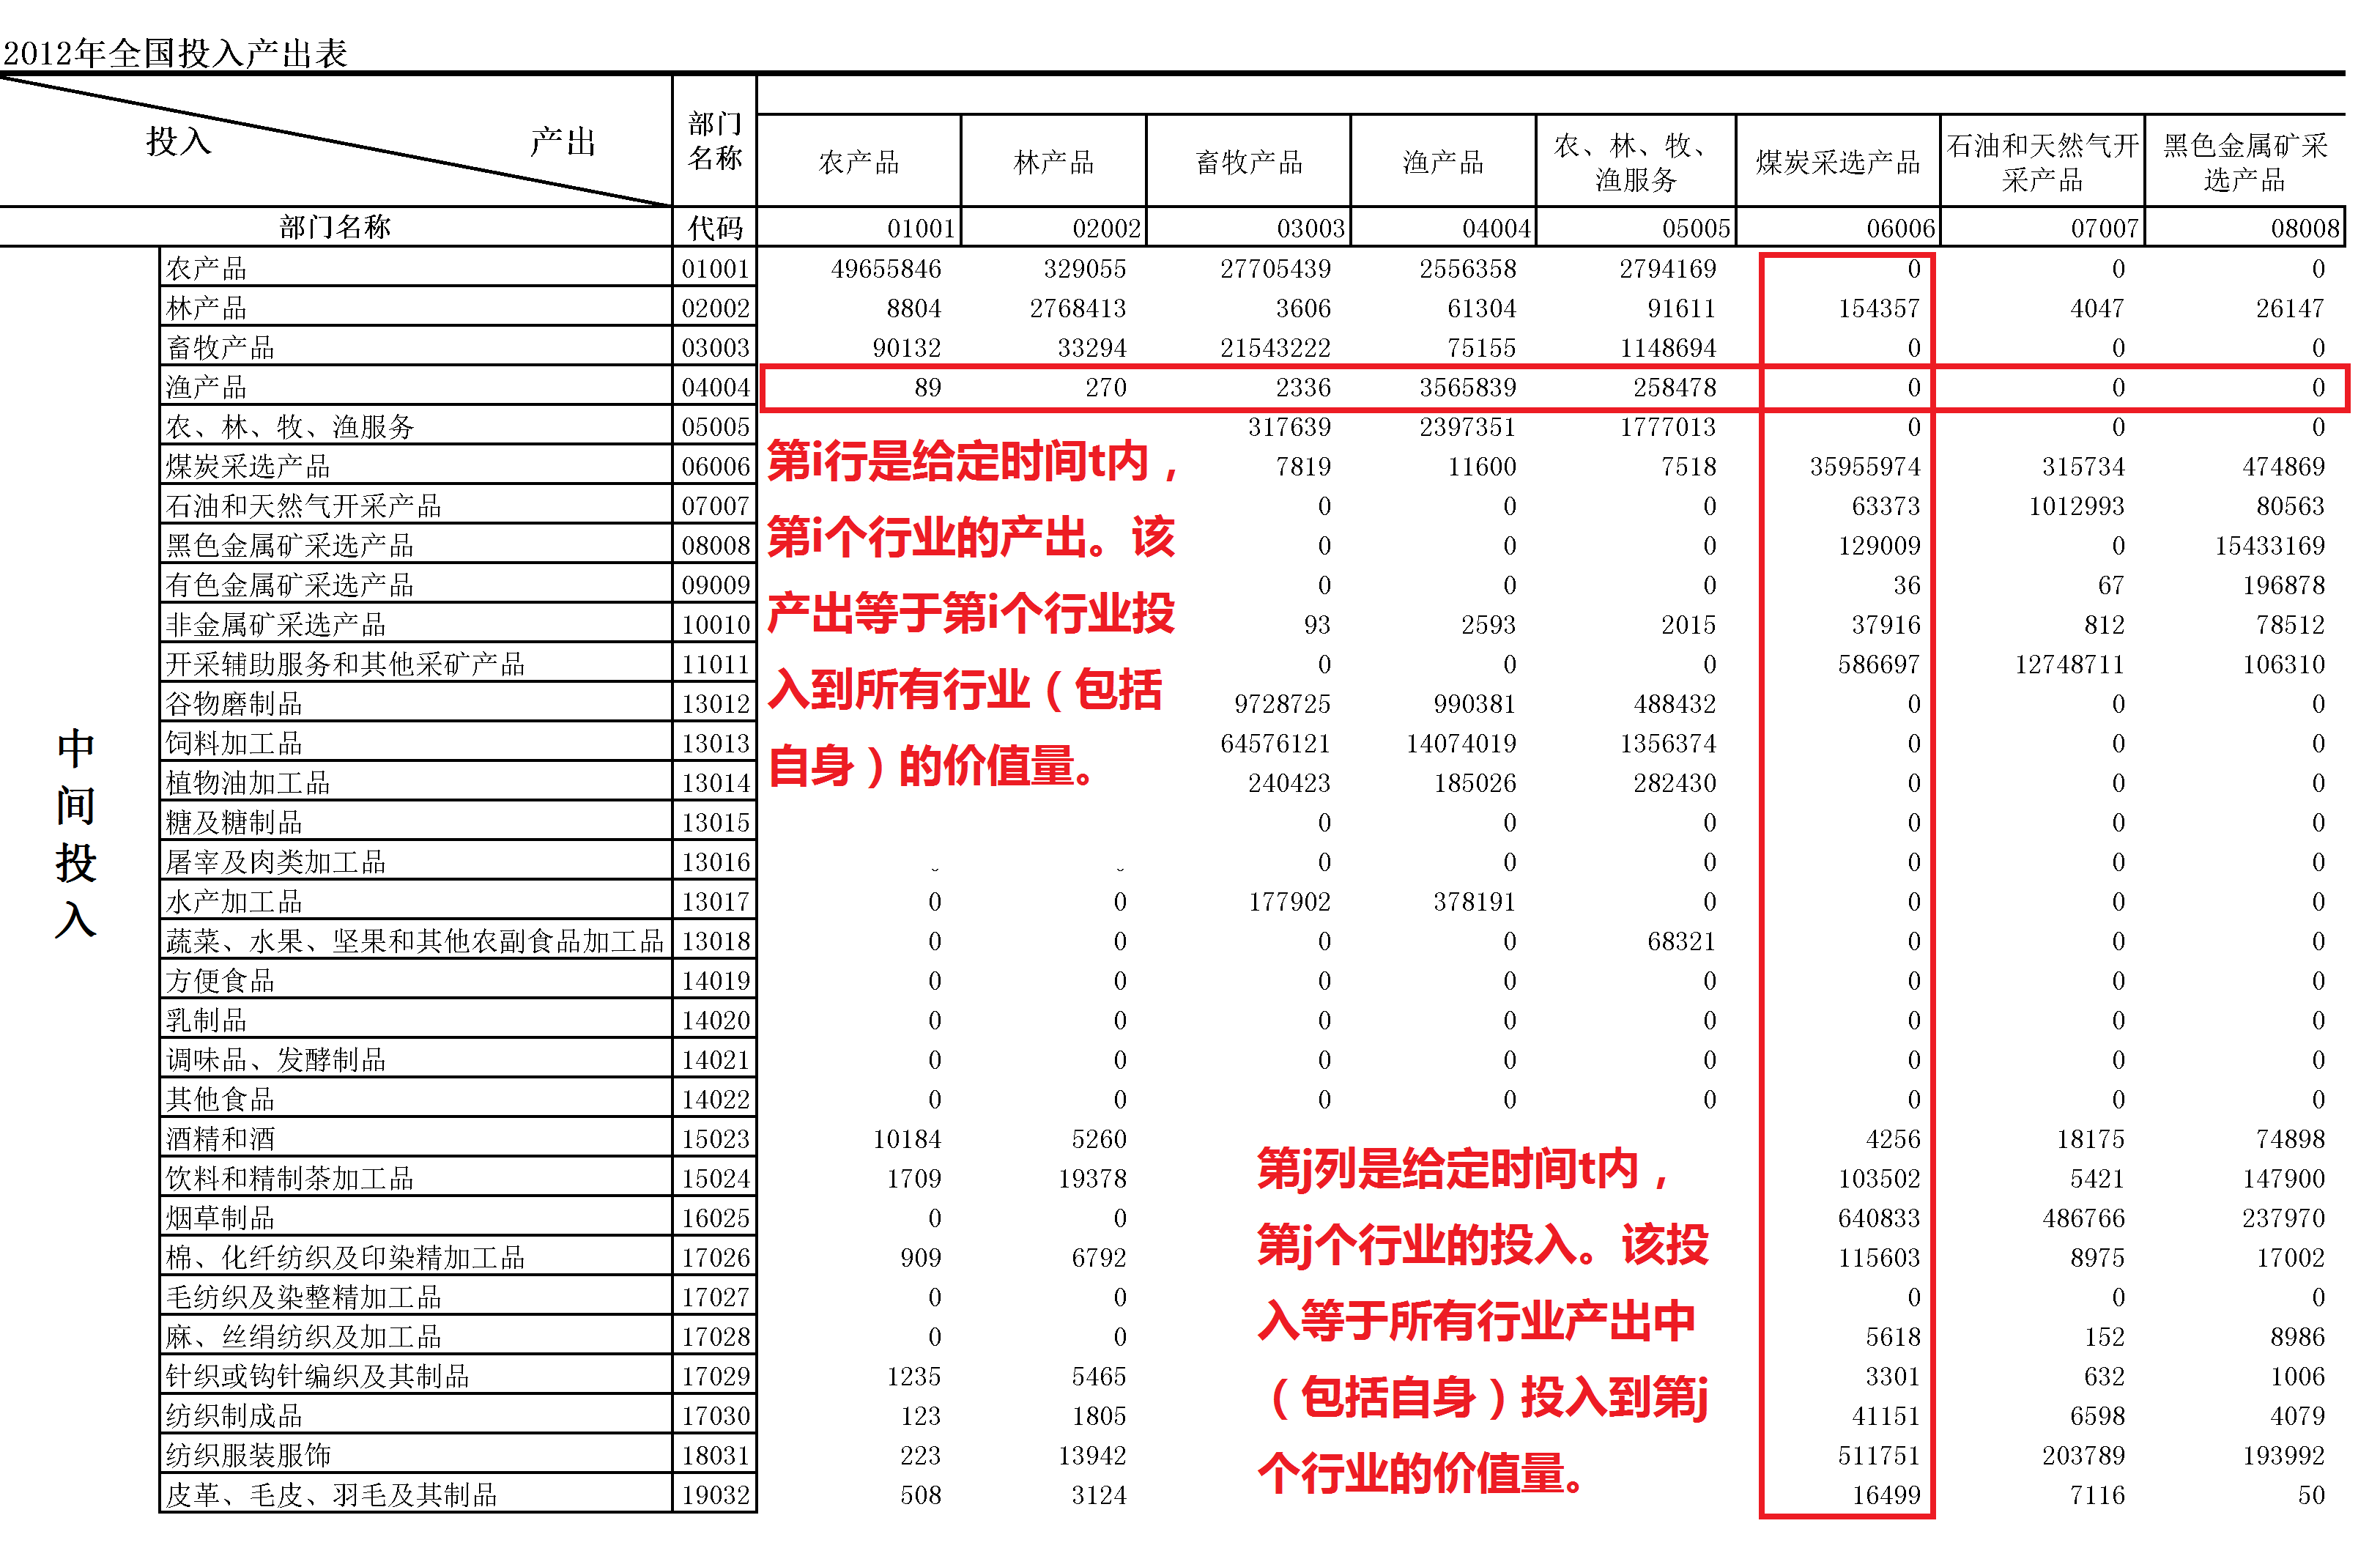
\includegraphics[scale=0.6]{image/2012-流量表中间投入部分.png}
  \caption{投入产出基表中间使用部分(节选图)}
  \caption*{\footnotesize 第I象限是本文数据采集的对象。投入产出表第I象限是中间投入的部分,主栏对应中间投入,宾栏对应中间使用。中间投入部分是一个$n \times n$的方阵,$n$是当年投入产出表中行业的总数。第i行为第i个行业在统计时间段内对各个行业的产出量。第j列是第j个行业在统计时间段内依赖各个行业的投入量。}
  \label{fig:ioaccount-quardone}
  \end{figure}

  \begin{figure}[h!tbp]
  \centering
  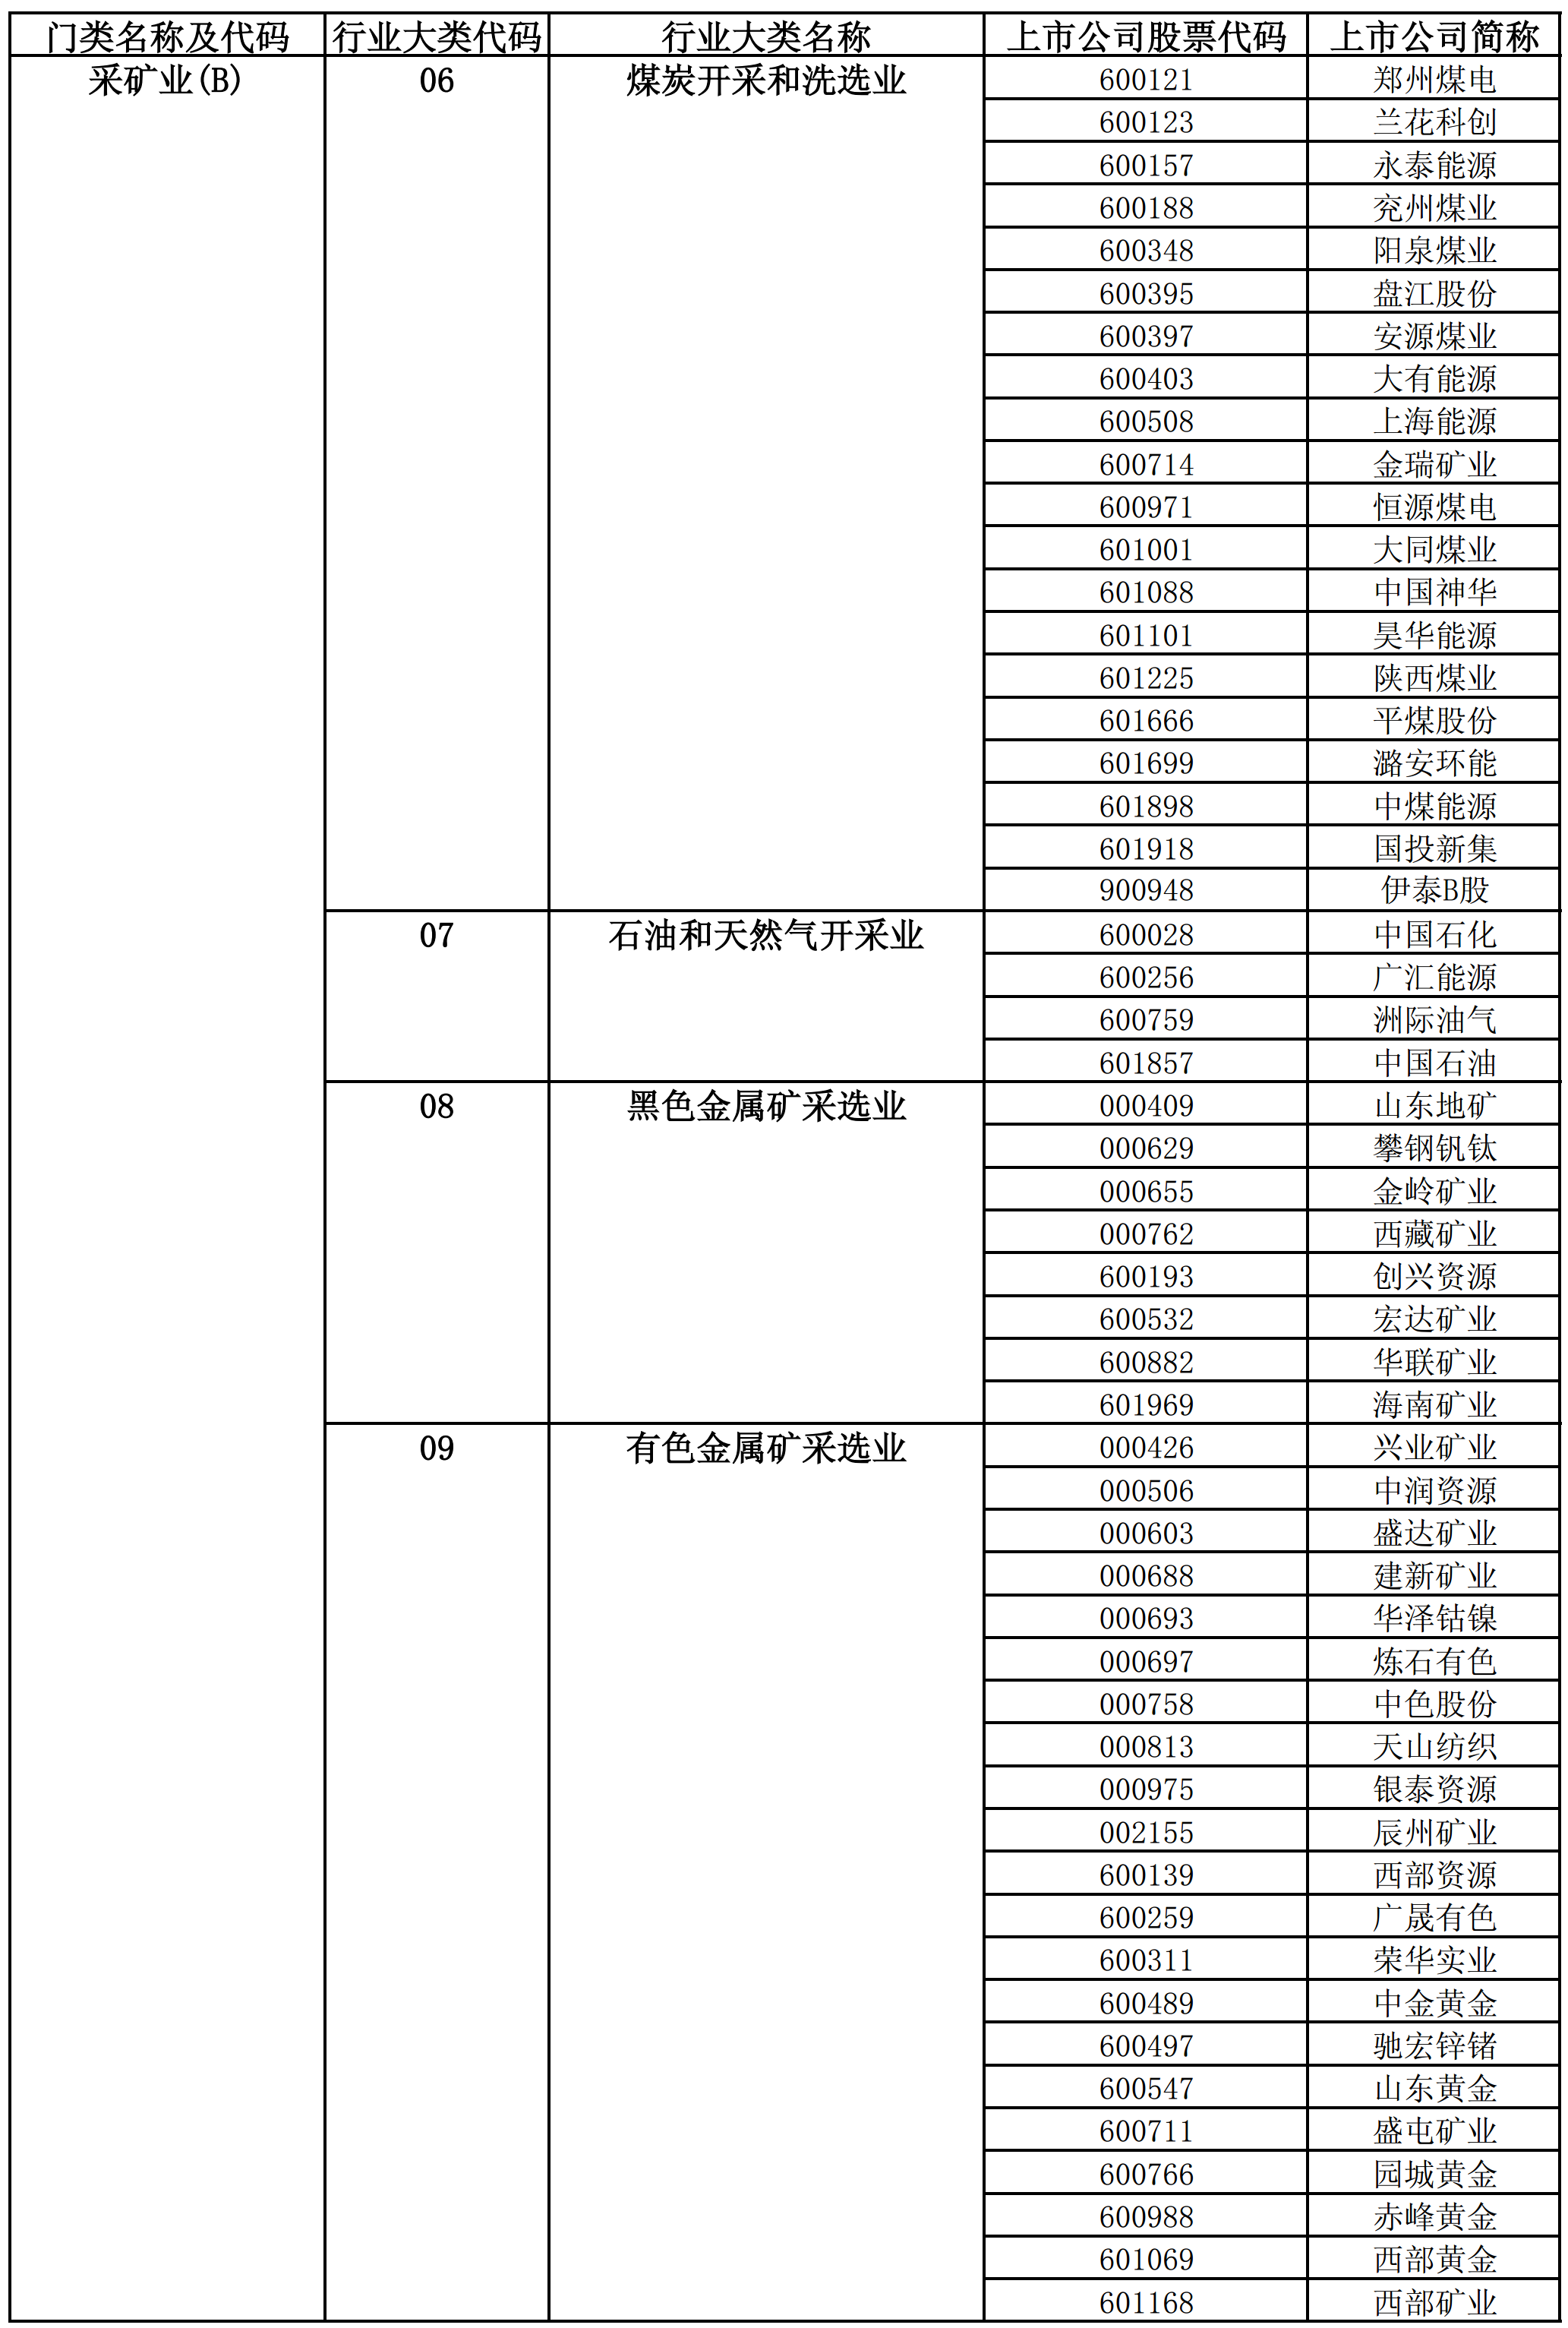
\includegraphics[scale=0.6]{image/2015年4季度上市公司行业分类结果.png}
  \caption{证监会上市公司行业分类结果(节选图)}
  \caption*{\footnotesize 该表格为证监会建立的上市公司行业分类结果的节选,分类建立的时间点是2015年第4季度,分类对象是在深圳和上海证券交易所挂牌上市的上市公司全体。表格的第一列是门类名称和代码,第二列是行业大类代码,第三列是行业大类名称,第四列是上市公司股票代码,第五列是上市公司的名称。}
  \label{fig:classify-output}
  \end{figure}

  \begin{figure}[htbp]
  \centering
  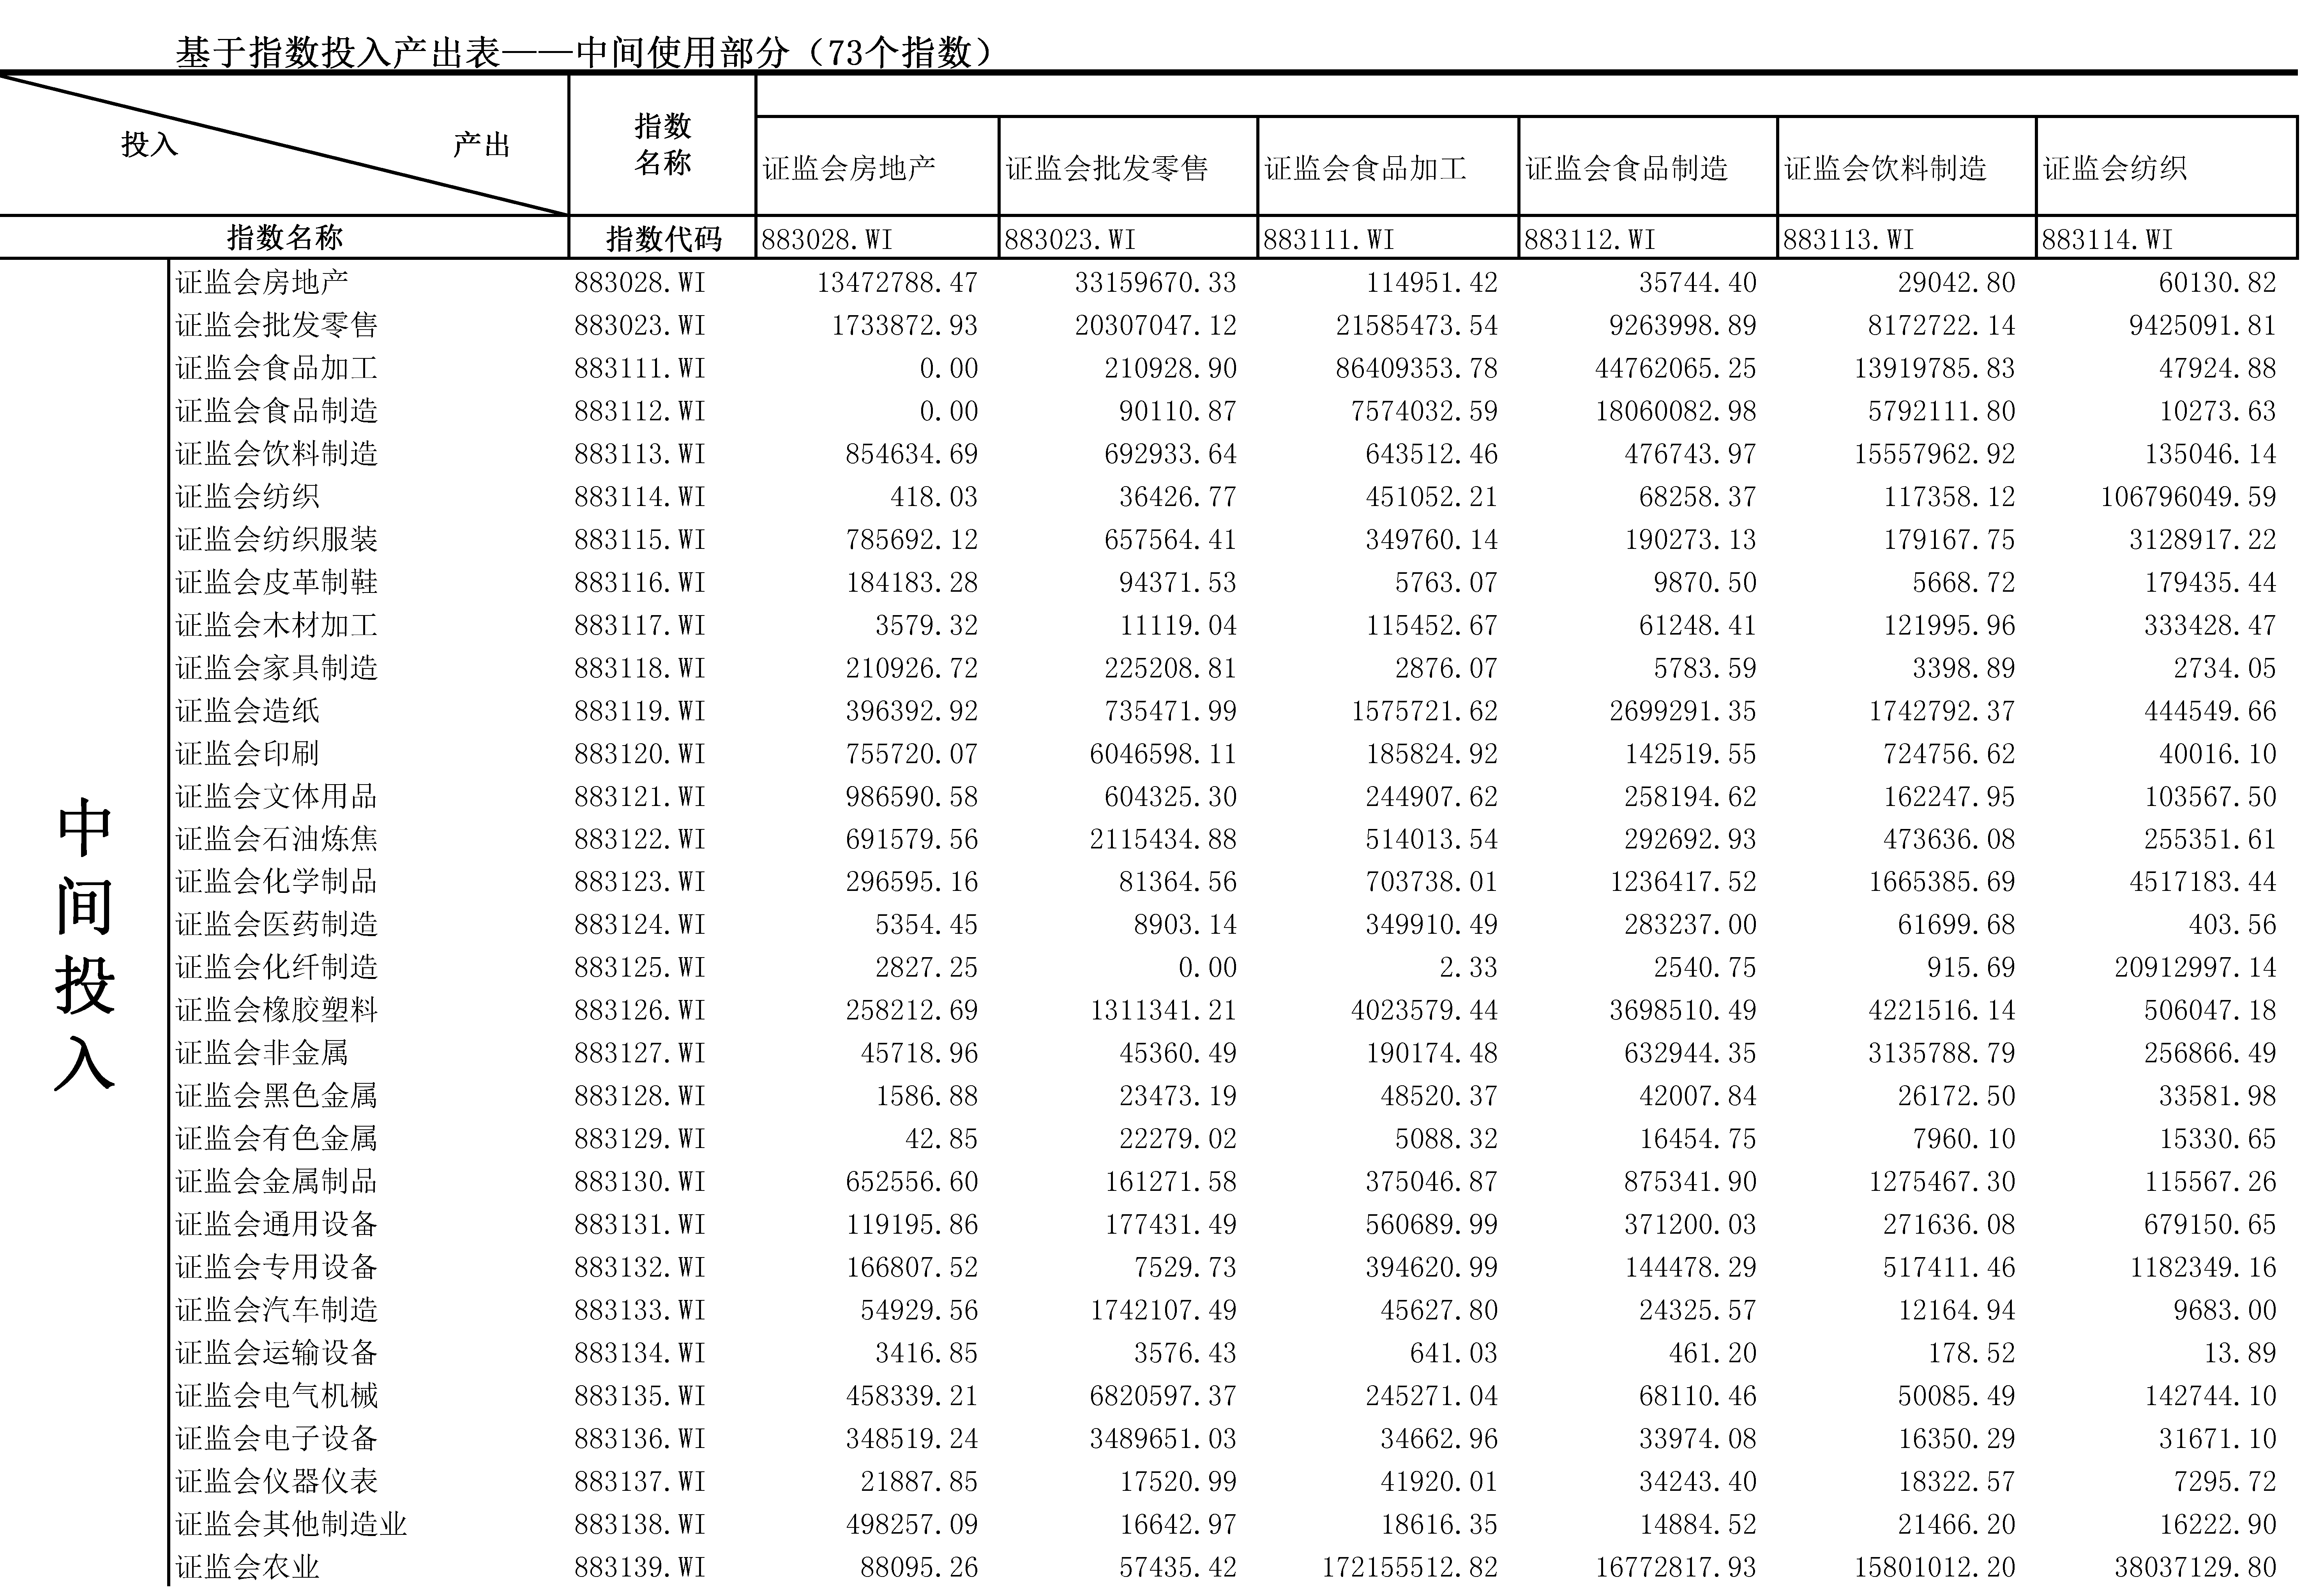
\includegraphics[scale=0.6]{image/合并调整后的中间流量表.png}
  \caption{合并调整后的行业指数的中间流量表(节选图)}
  \caption*{\footnotesize 合并调整后的行业指数的中间流量表是一个$n \times n$的方阵,$n$是当年证监会二级分类下行业指数的总数。第i行为第i个行业指数对应的行业在统计时间段内对其他行业指数对应的各个行业的产出量。第j列是第j个行业指数在统计时间段内对应的行业依赖各个行业指数对应的行业的投入量。}
  \label{fig:reorganized-ioaccount}
  \end{figure}

\subsection {指标选取} 
本文以周波动率及周收益率作为观测指标,解释被观测的指数波动的溢出现象。周数据是一个噪音与信号的权衡。在本文探究目标的角度而言,噪音是投资者短期投资策略变动导致的股价波动,信号是基于行业间信息扩散,影响投资者的决策,继而反映为指数价格的变化。周数据为捕捉这一信号提供了较为充足的样本,另一方面,周数据减缓了噪音的影响。

\subsection {数据清洗}
本节主要围绕采集数据指标时产生的问题,提出可行的解决方案,给出采取解决方案的原因。

选取周为数据的采样单位,需要考虑周末效应对数据结果的影响。周末效应是指股票在下一周周一的开盘价与上一周周末价格收盘价的偏离程度显著大于两个相邻交易日间的偏离程度的现象。这一现象客观存在的原因可以是由于在周末发布的影响股价价格变化的信息在下一周的周一的交易日中集中反映。因此,缓解这一现象的方法是将周末效应的信息纳入估计当中,对于每一周的数据,我们取该周的周三为起点,下一周的周二为终点作为周的划分标准,以减缓周末效应对模型的影响。

除了周末以外,重大节假日相关的信息也会影响数据结果。例如,对于旅游行业和零售批发行业,对将要到来的“黄金周”的销售数据的估计,可能通过影响相关行业上司公司的营业收入的估计,既而影响相关股价和行业指数。但是,在节假日期间,股市休市,这些信息无法充分地在市场中影响价格。具体表现为,一些横跨公众假日的采集区间中,一周选取到少于五个交易日的收益率样本,甚至只有一个交易日收益率样本。样本数量不足为波动率计算带来了不便。为了克服这一问题,我们将这些一个收益率样本的周数据,结合上一周的样本,计算这一时间段的波动率。结合上一周数据的合理之处在于,对于市场中的投资者而言,重大节假日的存在是已知的信息,出于逐利,他们会尽可能地响应节假日中的信息,既而影响股价。然而,上一周的价格与重大节假日所在的周的价格相比,后者对数据影响更大,因此,我们引入权重,放大后者取得的数据的影响。对收益率作加权处理后,也使得波动率增大以符合实际的观测。计算时周收益率和周波动率时,满足式\ref{yield-weighted}以及式\ref{volatility-weighted}。

\begin{equation}
\label{yield-weighted} 
{r'_t} = \lambda {r_t} + \frac{1}{\lambda }{r_{t-1}}
\end{equation}

${r'_t}$是调整后的本周对数收益率序列,${r_t}$是本周未调整时的对数收益率序列,${r_{t - 1}}$是上一周的对数收益率序列,$\lambda$是权重,它是一个大于1的实数,本文取$\lambda=3$,适当放大未调整的本周对数收益率的影响。由此得到数据不足的情况下,本周的波动率${r'_t}$。得到调整的收益率后,计算调整后的本周的波动率(年化),计算公式为式\ref{volatility-weighted}

\begin{equation}
\label{volatility-weighted} 
{\sigma '_t} = \sqrt {\frac{{\sum\limits_{i = 1}^N {{{({{r'}_{t,i}} - {{\bar r'}_t})}^2}} }}{{N - 1}}}  \times \sqrt {\frac{1}{{\Delta t}}}
\end{equation}

${\sigma '_t}$是调整后的本周年化波动率。${{\bar r'}_t}$是调整后的本周对数收益率的均值,$N$是调整后的本周对数收益率序列中交易日的天数。$\sqrt {\frac{1}{{\Delta t}}}$是年化因子,${\Delta t}$一年中交易天数的倒数,本文取年交易日天数为240。

\chapter{数据分析}

本章解决一个很重要的问题,如果捕捉到一个板块的利好,或者利空的消息,投资者应该选择哪些关联的企业作为我投资的对象,并且如何分配购置这些行业相关股票的比重。解决这个问题后,再引入刻画溢出效应的模型的假设和背景,解读回归模型基于最小二乘估计的结果,探究模型估计结果的参数敏感性以及模型的稳健性。

\section{模型假设}

投资者由于精力和能力的有限,往往没有办法立刻捕捉到影响股价的与行业自身相关的,以及行业链中相关行业的信号。若信号未能及时反应在股价的变化上,随着时间的推移,这些信号的影响将扩散到相关的行业,这表现为产业间收益率存在溢出效应。

在同一个时间点内,若行业间的中间使用部分的产出的价值量或中间使用部分的投入的价值量越大,则行业间的客观联系越紧密。

我们可以根据该时间段内的投入产出表,推断附近的时间段中,行业间相关上市公司股票相互关联的程度,相互关联程度越高,股价的溢出现象越明显。

\section{模型构建}

\subsection{获取上游和下游行业关联最密切的指数}

为了选择关联的企业作为投资对象,需要采集基于行业指数的中间流量表内的数据,也就是图\ref{fig:reorganized-ioaccount}。思路是将一个需要研究的行业,定位出它所在的指数,再根据这个指数中间流量表中的强度,分别按所在指数的行和列排序,得到与之关联最强的上游行业对应的指数,以及与之关联最强的下游行业对应的指数。例如,对于饲料生产相关的行业,我们先查询它在投入产出表中对应的行业为饲料加工业,得到它在2012版的投入产出表中的行业代号是13013,再根据表\ref{fig:iomapping}查询该行业代号对应的行业指数为证监会食品加工,再根据中间流量表\ref{fig:reorganized-ioaccount}排序,取上游和下游行业指数各5个,结果如表\ref{siliao-table}所示。
% 为了更直观地说明取上下游行业指数的特点,本文还分别取房地产行业和黑色金属制造行业的上游和下游的行业的流量为例,结果见表\ref{fangdichan-table}以及表\ref{heisejinshu-table}。

\begin{table}[!htbp] \centering 
  \caption{食品加工行业指数关联最密切的行业} 
  \caption*{\footnotesize 该表格选取了投入产出表中,与食品加工行业指数关联最密切的五个上游行业指数及五个下游行业指数。第一列是指数的交易代号;第二列为上述行业指数对应的行业在投入产出表中的中间流量,流量计算的时间段为2012年全年,计算单位为亿,精确到小数点后1位;第三列为流量在最密切的五个行业的总流量中所占比例,精确到小数点后3位。与食品加工指数关联最密切的五个上游行业的行业指数分别对应以下的五个行业:农业,畜牧业,渔业,批发零售业,道路运输业;与食品加工指数关联最密切的五个下游行业的行业指数分别对应以下的五个行业:畜牧业,食品制造业,餐饮业,渔业,饮料制造业。}
  \label{siliao-table} 
  \begin{tabular}{@{\extracolsep{5pt}} cccccc} 
  \\[-1.8ex]\hline 
  \hline \\[-1.8ex] 
   & 1 & 2 & 3 & 4 & 5 \\ 
  \hline \\[-1.8ex] 
  上游行业指数 & 883139.WI & 883141.WI & 883142.WI & 883023.WI & 883159.WI \\ 
  指数流量 & 17215.6 & 6491.4 & 2667.4 & 2158.5 & 856.8 \\ 
  指数比重 & 0.586 & 0.221 & 0.091 & 0.073 & 0.029 \\ 
  下游行业指数 & 883141.WI & 883112.WI & 883166.WI & 883142.WI & 883113.WI \\ 
  指数流量 & 7472.3 & 4476.2 & 4307.5 & 1562.8 & 1392 \\ 
  指数比重 & 0.389 & 0.233 & 0.224 & 0.081 & 0.072 \\ 
  \hline \\[-1.8ex] 
  \end{tabular} 
\end{table} 

% \begin{table}[!htbp] \centering 
%   \caption{房地产行业指数关联最密切的行业} 
%   \caption*{\footnotesize 该表格选取了投入产出表中,与房地产行业指数关联最密切的五个上游行业指数及五个下游行业指数。第一列是指数的交易代号;第二列为上述行业指数对应的行业在投入产出表中的中间流量,流量计算的时间段为2012年全年,计算单位为亿,精确到小数点后1位;第三列为流量在最密切的五个行业的总流量中所占比例,精确到小数点后3位。与房地产指数关联最密切的五个上游行业的行业指数分别对应以下的五个行业:货币金融服务业,商务服务业,建筑装饰业,电热生产供应业,批发零售业;与房地产指数关联最密切的五个下游行业的行业指数分别对应以下的五个行业:货币金融服务业,批发零售业,餐饮业,商务服务业,电信业。
% }
% \end{table} 
%   \label{fangdichan-table} 
%   \begin{tabular}{@{\extracolsep{5pt}} cccccc} 
%   \\[-1.8ex]\hline 
%   \hline \\[-1.8ex] 
%    & 1 & 2 & 3 & 4 & 5 \\ 
%   \hline \\[-1.8ex] 
%   上游行业指数 & 883170.WI & 883176.WI & 883155.WI & 883149.WI & 883023.WI \\ 
%   指数流量 & 4317.0 & 1649.6 & 854.7 & 202.6 & 173.4 \\ 
%   指数比重 & 0.6 & 0.229 & 0.119 & 0.028 & 0.024 \\ 
%   下游行业指数 & 883170.WI & 883023.WI & 883169.WI & 883176.WI & 883167.WI \\ 
%   指数流量 & 3436.3 & 3316.0 & 293.6 & 266.6 & 243.8 \\ 
%   指数比重 & 0.455 & 0.439 & 0.039 & 0.035 & 0.032 \\ 
%   \hline \\[-1.8ex] 
% \end{tabular} 

% \begin{table}[!htbp] \centering 
%   \caption{黑色金属行业指数关联最密切的行业} 
%   \caption*{\footnotesize 该表格选取了投入产出表中,与黑色金属行业指数关联最密切的五个上游行业指数及五个下游行业指数。第一列是指数的交易代号;第二列为上述行业指数对应的行业在投入产出表中的中间流量,流量计算的时间段为2012年全年,计算单位为亿,精确到小数点后1位;第三列为流量在最密切的五个行业的总流量中所占比例,精确到小数点后3位。与黑色金属行业指数关联最密切的五个上游行业的行业指数分别对应以下的五个行业:黑色金属矿采选业,石油炼焦业,煤炭开采业,废弃资源综合利用业,电热生产供应业;与黑色金属行业指数关联最密切的五个下游行业的行业指数分别对应以下的五个行业:房屋建筑业,金属制品业,土木工程建筑业,通用设备制造业,专用设备制造业。}
%   \label{heisejinshu-table} 
%   \begin{tabular}{@{\extracolsep{5pt}} cccccc} 
%   \\[-1.8ex]\hline 
%   \hline \\[-1.8ex] 
%    & 1 & 2 & 3 & 4 & 5 \\ 
%   \hline \\[-1.8ex] 
%   上游行业指数 & 883146.WI & 883122.WI & 883144.WI & 883189.WI & 883149.WI \\ 
%   指数流量 & 12500.2 & 4270.9 & 2590.8 & 2567.9 & 2426.8 \\ 
%   指数比重 & 0.513 & 0.175 & 0.106 & 0.105 & 0.1 \\ 
%   下游行业指数 & 883152.WI & 883130.WI & 883153.WI & 883131.WI & 883132.WI \\ 
%   指数流量 & 12979.4 & 8279.4 & 5801.8 & 5146.7 & 4116.8 \\ 
%   指数比重 & 0.357 & 0.228 & 0.16 & 0.142 & 0.113 \\ 
%   \hline \\[-1.8ex] 
%   \end{tabular} 
% \end{table} 

为了更直观地认识行业间关联的强度对行业指数的收益率和波动率的影响,再绘制相关行业的上游行业的收益率序列和波动率序列,与下游行业的收益率序列和波动率序列。收益率序列见图\ref{fig:883111-topk-upper-plus-one-weeklyyield-combined};图\ref{fig:883111-topk-upper-plus-one-weeklyyield-single};图\ref{fig:883111-topk-lower-plus-one-weeklyyield-combined};图\ref{fig:883111-topk-lower-plus-one-weeklyyield-single},波动率序列见图\ref{fig:883111-topk-upper-plus-one-weeklyvol-combined};图\ref{fig:883111-topk-upper-plus-one-weeklyvol-single};图\ref{fig:883111-topk-lower-plus-one-weeklyvol-combined};图\ref{fig:883111-topk-upper-plus-one-weeklyvol-single}

  \begin{figure}[htbp]
  \centering
  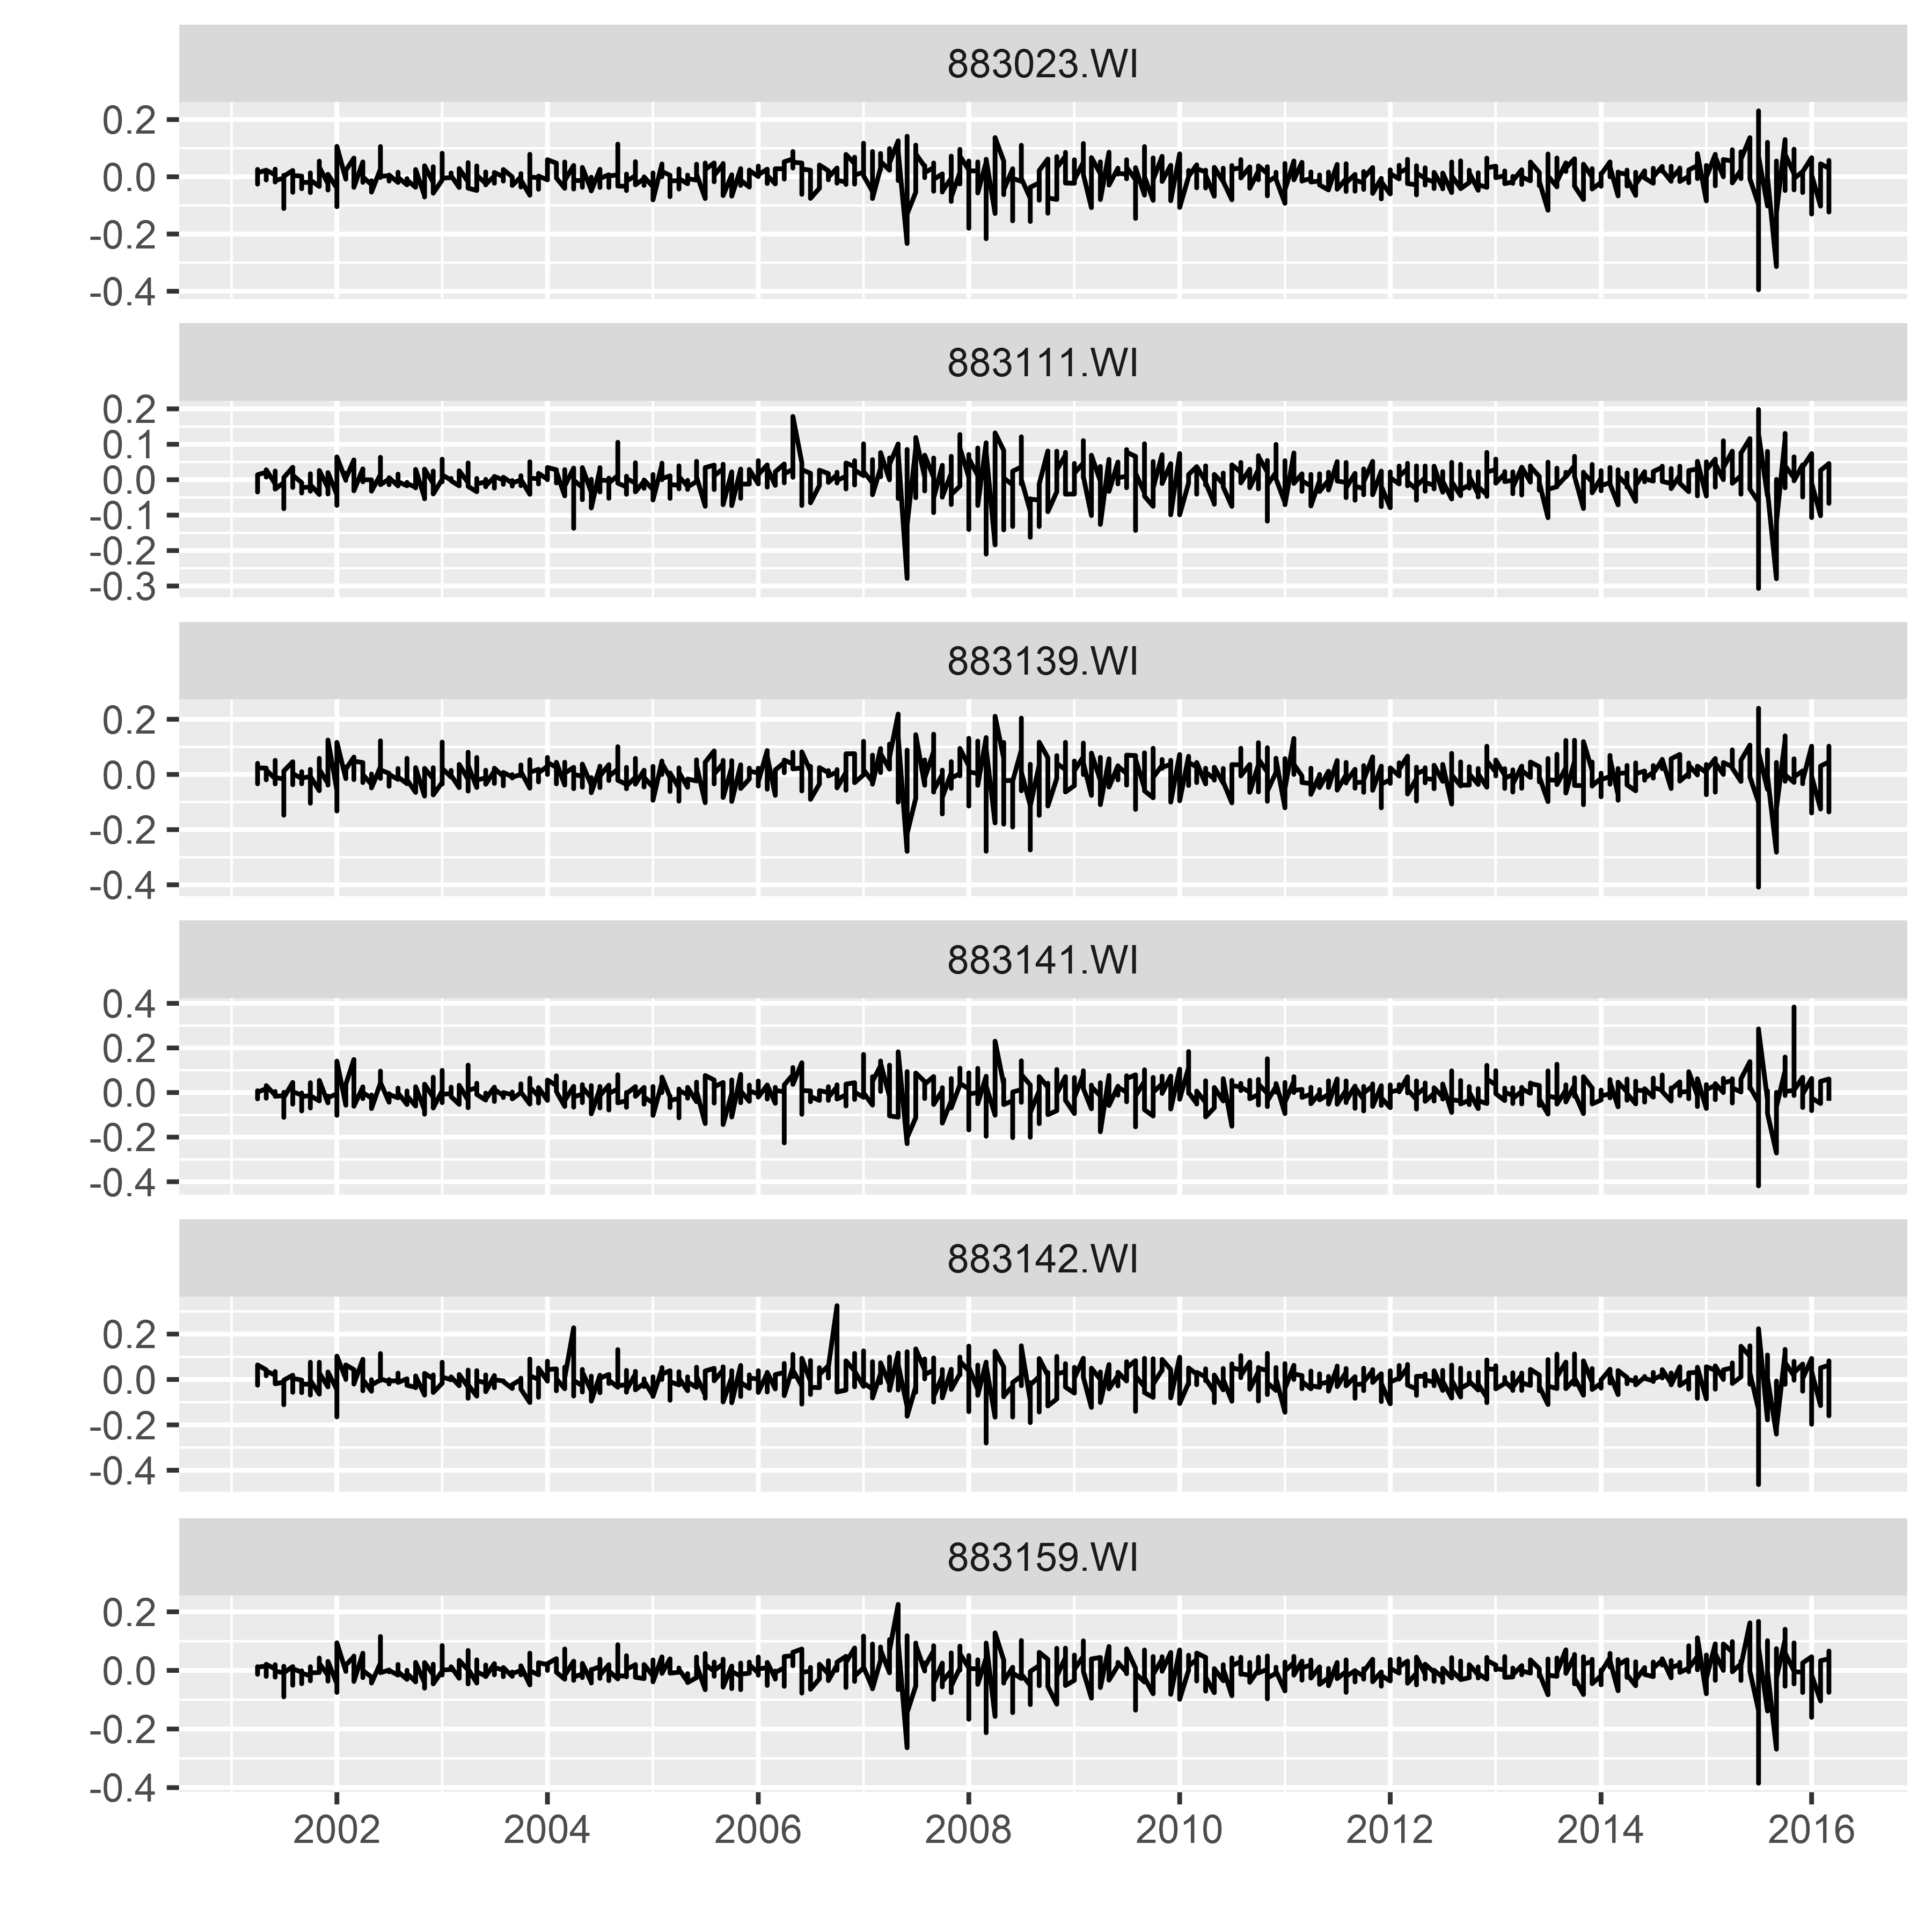
\includegraphics[scale=0.8]{image/883111-topk-upper-plus-one-weeklyyield-single.png}
  \caption{食品加工行业指数与关联最密切的五个上游行业指数的周收益率序列-指数分图列出}
  \caption*{\footnotesize 该图记录了食品加工行业指数与关联最密切的五个上游行业指数的周收益率的折线图,本图分为六张子图,其中,第一张子图是食品加工行业指数的周收益率序列,第二张到第六张子图是与食品加工行业关联最密切的五个上游行业指数的周收益率序列。每张子图的最上方是行业指数代号,$X$轴是时间,从2001年4月第一周开始,到2016年3月最后一周。$Y$轴是对数周收益率。}
  \label{fig:883111-topk-upper-plus-one-weeklyyield-single}
  \end{figure}

  \begin{figure}[htbp]
  \centering
  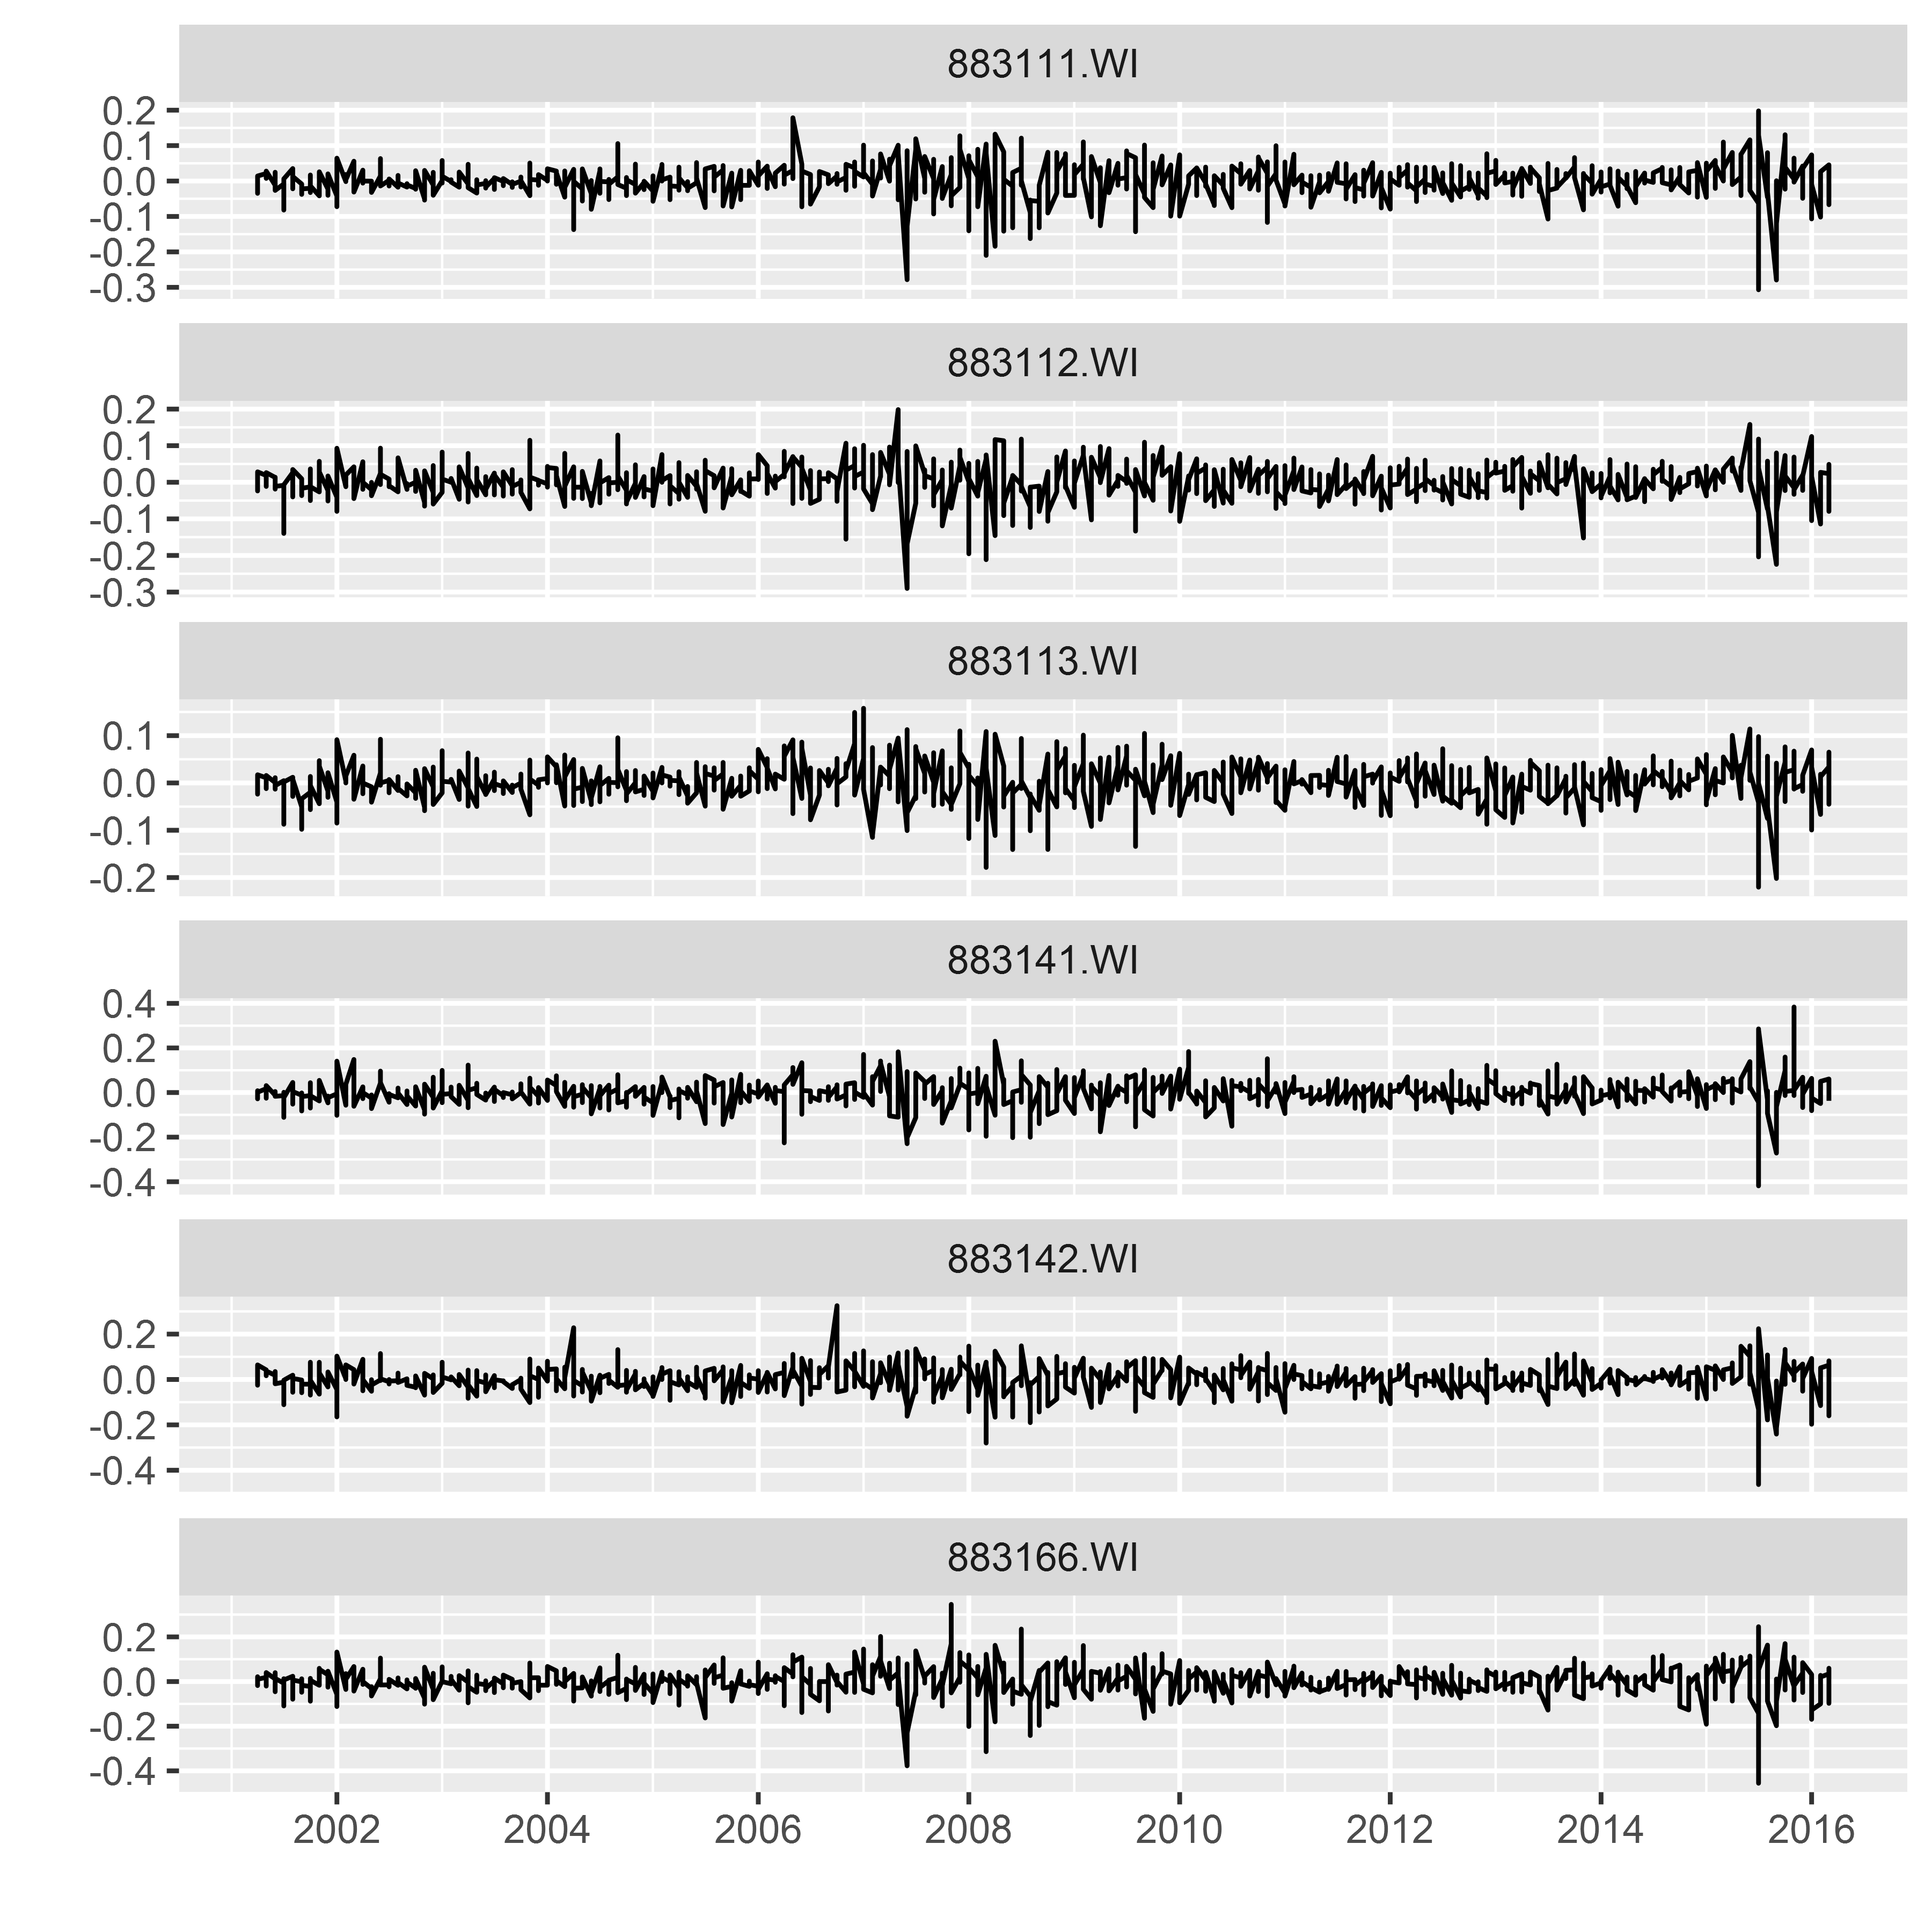
\includegraphics[scale=0.8]{image/883111-topk-lower-plus-one-weeklyyield-single.png}
  \caption{食品加工行业指数与关联最密切的五个下游行业指数的周收益率序列-指数分图列出}
  \caption*{\footnotesize 该图记录了食品加工行业指数与关联最密切的五个下游行业指数的周收益率的折线图,本图分为六张子图,其中,第一张子图是食品加工行业指数的周收益率序列,第二张到第六张子图是与食品加工行业关联最密切的五个下游行业指数的周收益率序列。每张子图的最上方是行业指数代号,$X$轴是时间,从2001年4月第一周开始,到2016年3月最后一周。$Y$轴是对数周收益率。}
  \label{fig:883111-topk-lower-plus-one-weeklyyield-single}
  \end{figure}


  \begin{figure}[htbp]
  \centering
  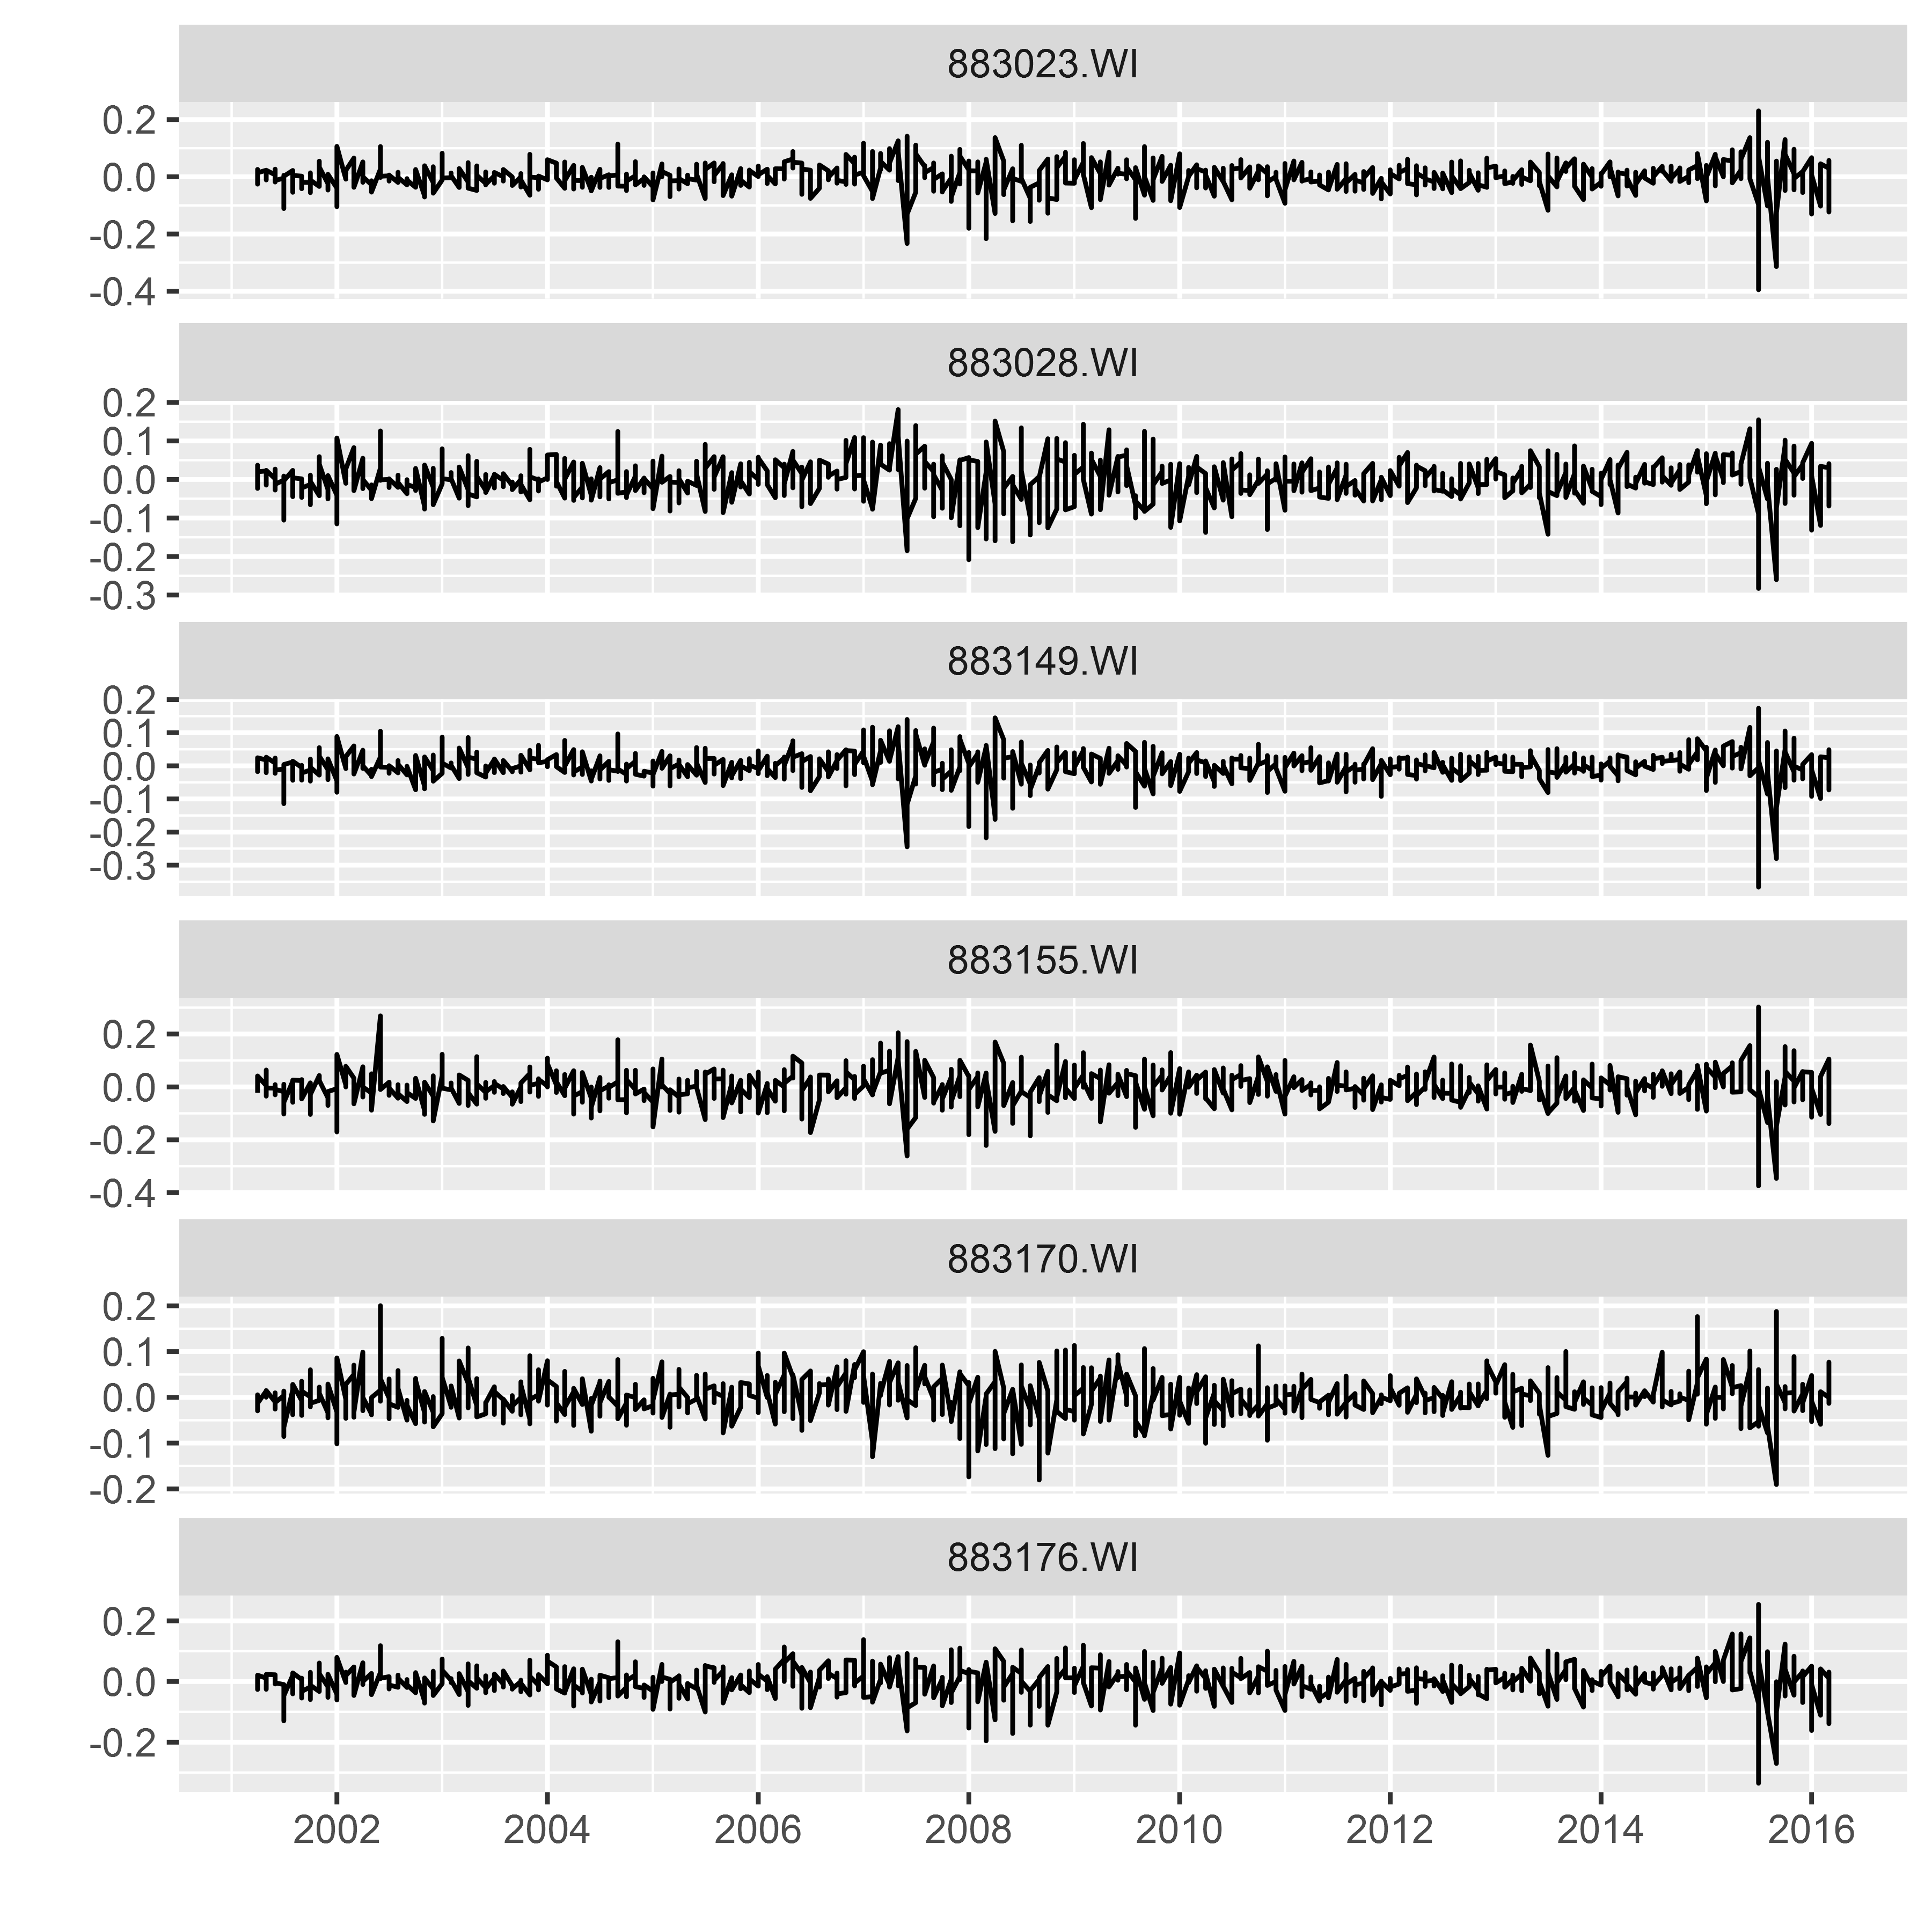
\includegraphics[scale=0.8]{image/883111-topk-upper-plus-one-weeklyvol-single.png}
  \caption{食品加工行业指数与关联最密切的五个上游行业指数的周波动率(年化)序列-指数分图列出}
  \caption*{\footnotesize 该图记录了食品加工行业指数与关联最密切的五个上游行业指数的年化周波动率的折线图,本图分为六张子图,其中,第一张子图是食品加工行业指数的年化周波动率序列,第二张到第六张子图是与食品加工行业关联最密切的五个上游行业指数年化的历史周波动率序列。每张子图的最上方是行业指数代号,$X$轴是时间,从2001年4月第一周开始,到2016年3月最后一周。$Y$轴是年化的历史周波动率。}
  \label{fig:883111-topk-upper-plus-one-weeklyvol-single}
  \end{figure}


  \begin{figure}[htbp]
  \centering
  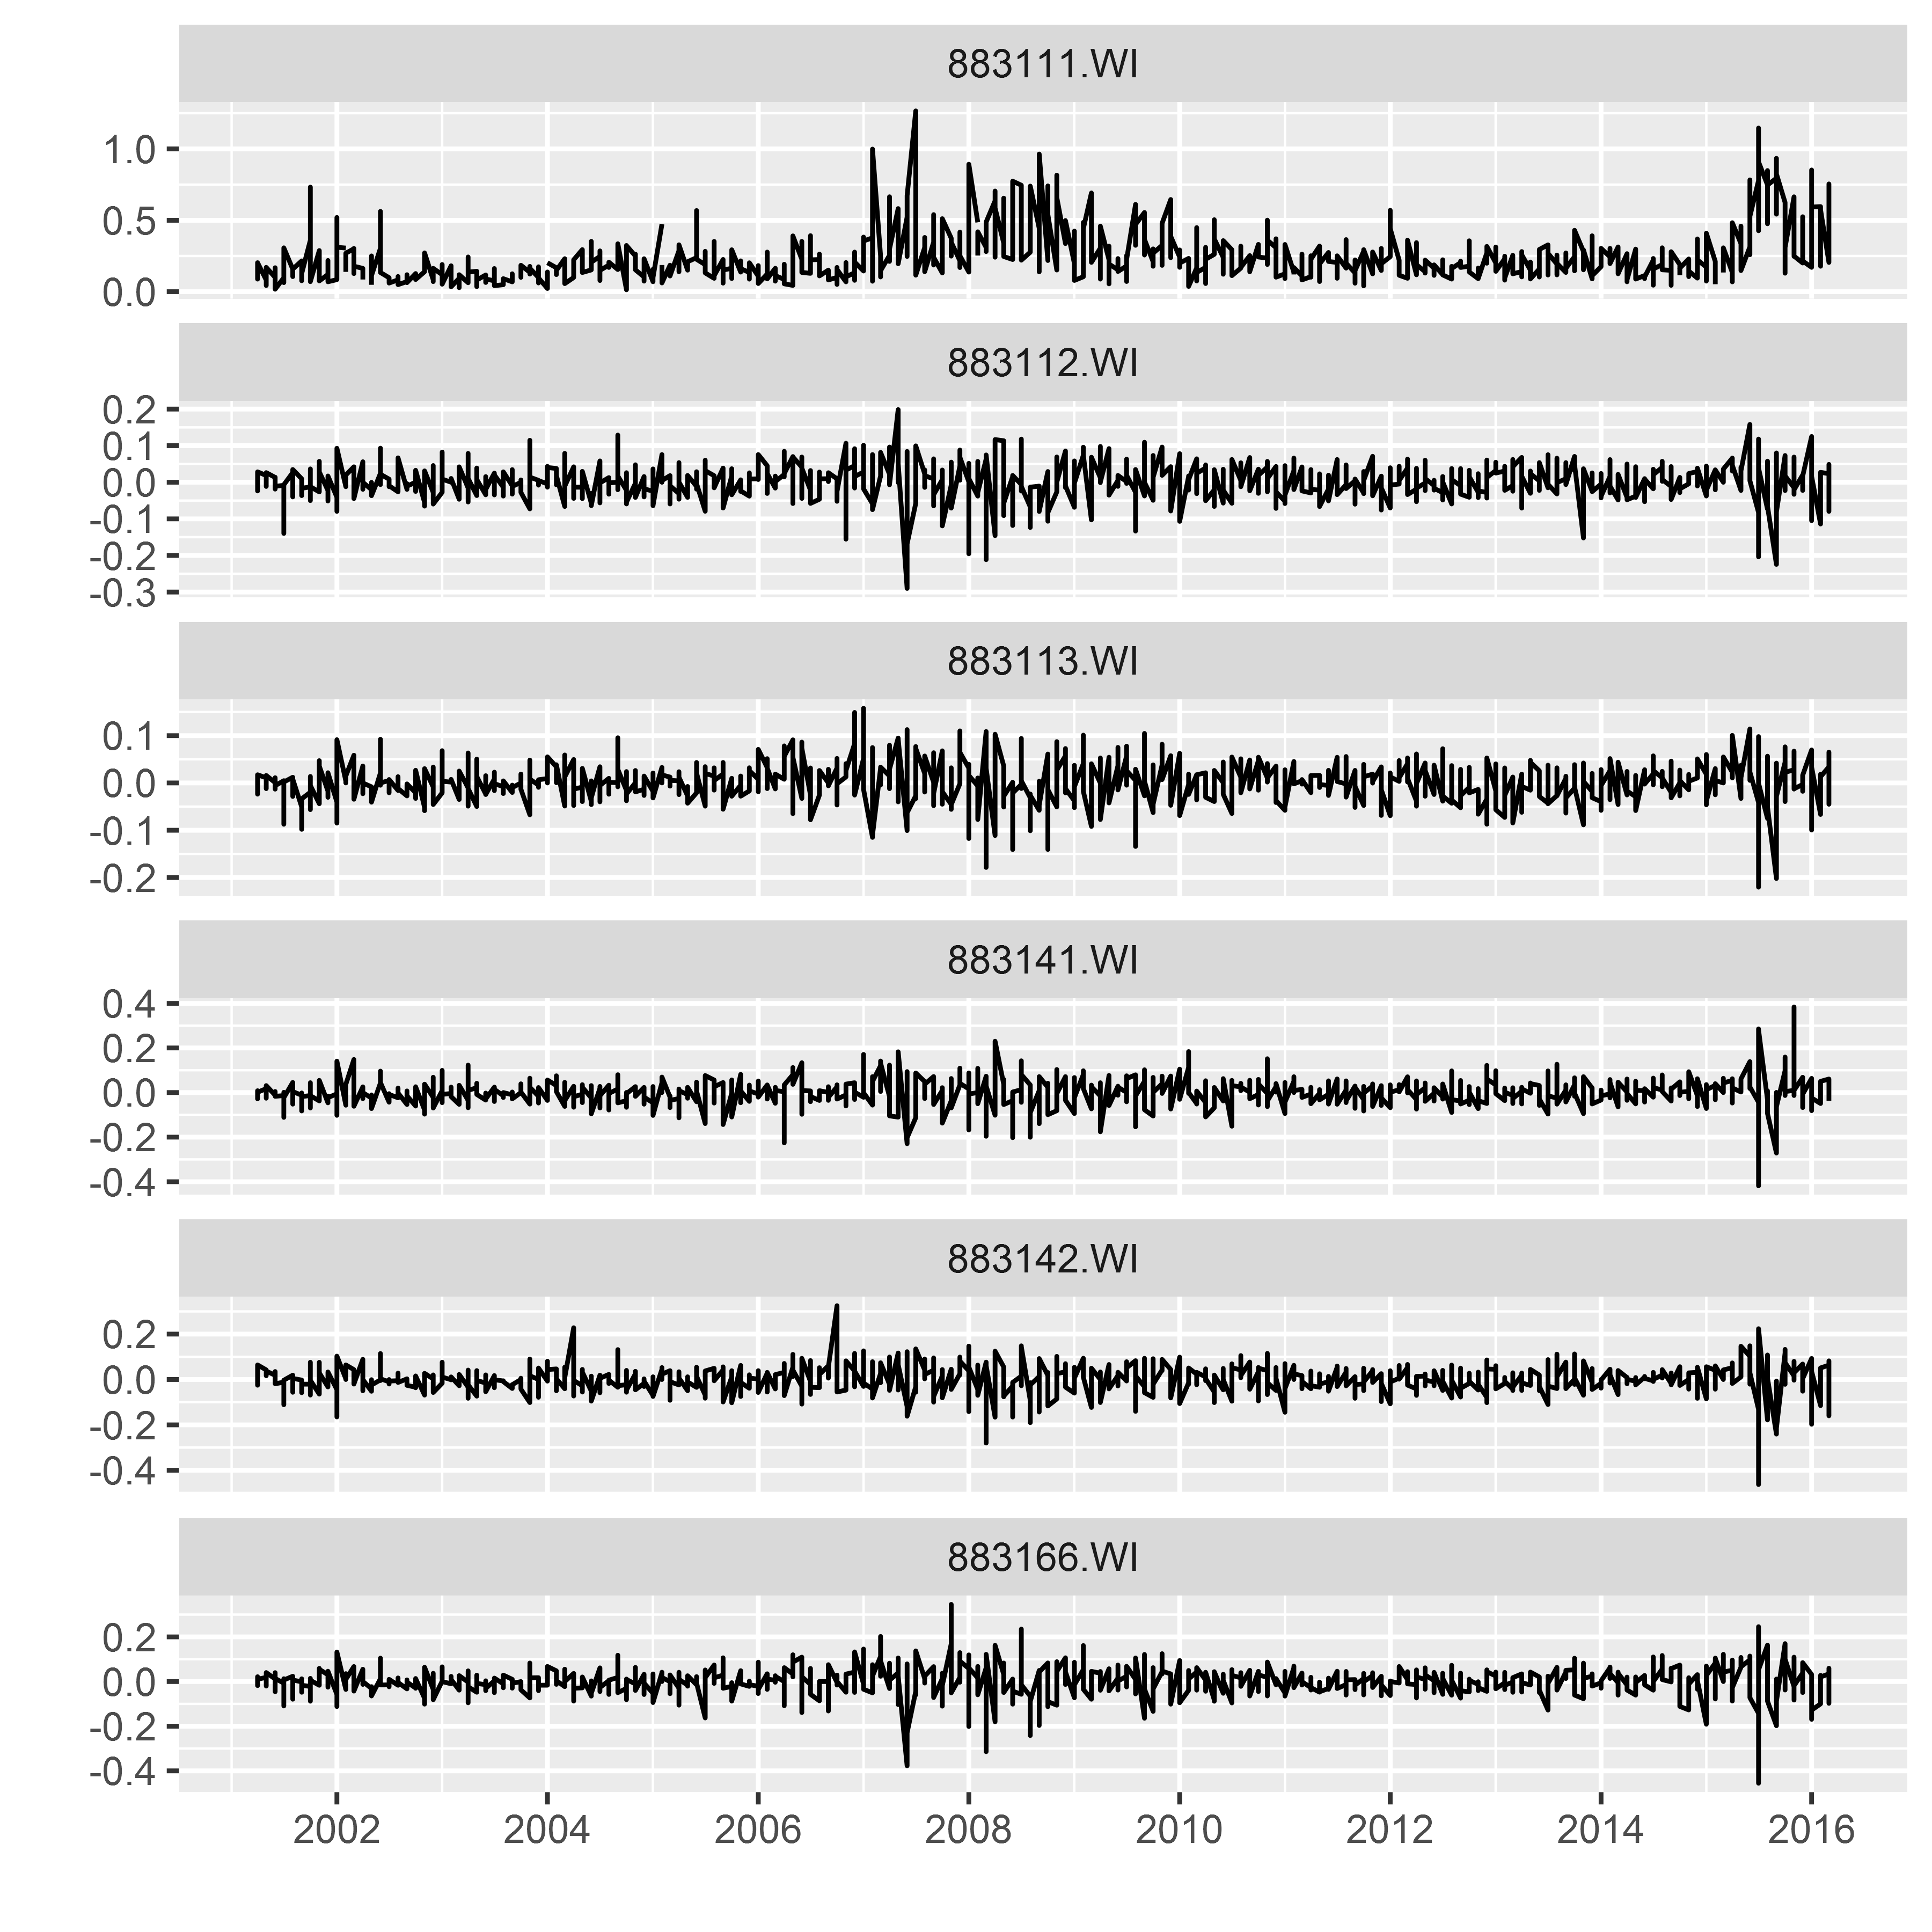
\includegraphics[scale=0.8]{image/883111-topk-lower-plus-one-weeklyvol-single.png}
  \caption{食品加工行业指数与关联最密切的五个下游行业指数的周波动率(年化)序列-指数分图列出}
  \caption*{\footnotesize 该图记录了食品加工行业指数与关联最密切的五个下游行业指数的年化周波动率的折线图,本图分为六张子图,其中,第一张子图是食品加工行业指数的年化周波动率序列,第二张到第六张子图是与食品加工行业关联最密切的五个下游行业指数年化的历史周波动率序列。每张子图的最上方是行业指数代号,$X$轴是时间,从2001年4月第一周开始,到2016年3月最后一周。$Y$轴是年化的历史周波动率。}
  \label{fig:883111-topk-lower-plus-one-weeklyvol-single}
  \end{figure}

\subsection{获取上游和下游行业指数的波动率和收益率序列}
为了进一步利用投入产出表中的信息,我们希望利用投入产出表中的中间流量,为构建资产组合提供权重。因此,根据流量强度,分别构建上游的波动率序列和下游的波动率序列,公式见\ref{yield-upper-recombined}以及\ref{yield-lower-recombined}。

\begin{equation}
\label{yield-upper-recombined} 
{r’_{upper}} = \sum\limits_{i = 1}^k {{r_{upper,i}}{w_i}} 
\end{equation}

${r’_{upper}}$是组合后的上游行业的对数收益率序列,${r_{upper,i}}$是上游行业中,联系最大的第i个行业对应的行业指数的对数收益率序列,$k$是除去自身以外,囊括的行业指数的数量,${w_i}$则为第$i$个指数的中间流量权重。

\begin{equation}
\label{yield-lower-recombined} 
{r’_{lower}} = \sum\limits_{i = 1}^k {{r_{lower,i}}{w_i}} 
\end{equation}

${r’_{lower}}$是组合后的下游行业的对数收益率序列,${r_{lower,i}}$是下游行业中,联系最大的第i个行业对应的行业指数的对数收益率序列,$k$是除去自身以外,囊括的行业指数的数量,${w_i}$则为第$i$个指数的中间流量权重。

思路是根据流量权重,分别构建上游和下游的收益率序列,再根据新组合的资产组合的收益率序列,计算它的波动率。例如,食品加工行业指数,与其加权上游行业指数和其加权下游行业指数的收益率序列和波动率序列,得到组合后的上游和下游的对数收益率序列后,计算其波动率,计算公式见\ref{volatility-upper-recombined},以及式\ref{volatility-lower-recombined}。

\begin{equation}
\label{volatility-upper-recombined} 
{\sigma '_{upper,t}} = \sqrt {\frac{{\sum\limits_{i = 1}^N {{{({{r'}_{upper,t,i}} - {{\bar r'}_{upper,t}})}^2}} }}{{N - 1}}}  \times \sqrt {\frac{1}{{\Delta t}}} 
\end{equation}

${\sigma '_{upper,t}} $是组合后的上游行业在时间点$t$的年化波动率。${{\bar r'}_{upper,t}}$是组合后的上游行业的在时间$t$的周对数收益率的均值,$N$是组合后的上游行业的周对数收益率序列中交易日的天数。$\sqrt {\frac{1}{{\Delta t}}}$是年化因子,${\Delta t}$一年中交易天数的倒数,本文取年交易日天数为240。

\begin{equation}
\label{volatility-lower-recombined} 
{\sigma '_{lower,t}} = \sqrt {\frac{{\sum\limits_{i = 1}^N {{{({{r'}_{lower,t,i}} - {{\bar r'}_{lower,t}})}^2}} }}{{N - 1}}}  \times \sqrt {\frac{1}{{\Delta t}}} 
\end{equation}

${\sigma '_{lower,t}} $是组合后的下游行业在时间点$t$的年化波动率。${{\bar r'}_{lower,t}}$是组合后的下游行业的在时间$t$的周对数收益率的均值,$N$是组合后的下游行业的周对数收益率序列中交易日的天数。$\sqrt {\frac{1}{{\Delta t}}}$是年化因子,${\Delta t}$一年中交易天数的倒数,本文取年交易日天数为240。

\section{衡量溢出效应}
若溢出效应存在,那么,待研究的行业指数在该时间点的收益率或波动率,一定程度上可被该时间点前的上游行业指数和下游行业指数分别解释。例如,饲料生产行业所在的食品加工行业指数在给定时间点$t$的收益率和波动率,可以被包括猪养殖业所在的畜牧业指数在前一时间点$t-1$的收益率和波动率解释。统计上,即待研究的行业指数到时间$t$的序列作因变量,而它的加权上游行业指数和加权下游行业指数到时间$t-1$的序列作解释变量,即满足式\ref{least-square-yield}即式\ref{least-square-yield}即式\ref{least-square-volatility}。

\begin{equation}
\label{least-square-yield}
{{r}_t} = {\beta _{upper}}{{r'}_{upper,t - 1}} + {\beta _{lower}} {{r'}_{lower,t - 1}} + {{e}_t}
\end{equation}

${{r}_t}$是待研究行业在时间点$t$的收益率,${{\r '}_{upper,t - 1}}$是组合后的上游行业在时间点$t-1$的收益率,${{\r '}_{lower,t - 1}}$是组合后的下游行业在时间点$t-1$的收益率序列,${\beta _{upper}}$和${\beta _{lower}}$分别是组合后的上游行业在时间点$t-1$的收益率和组合后的下游行业在时间点$t-1$的收益率的最小二乘估计。

\begin{equation}
\label{least-square-volatility}
{{\sigma }_t} = {\beta _{upper}}{{\bf{\sigma '}}_{upper,t - 1}} + {\beta _{lower}} {{\sigma '}_{lower,t - 1}} + {{e}_t}
\end{equation}

${{\sigma }_t}$是待研究行业在时间点$t$的年化波动率,${{\sigma '}_{upper,t - 1}}$是组合后的上游行业在时间点$t-1$的年化波动率,${{\sigma '}_{lower,t - 1}}$是组合后的下游行业到时间点$t-1$的年化波动率,${\beta _{upper}}$和${\beta _{lower}}$分别是组合后的上游行业的时间序列和组合后的下游行业的年化波动率的最小二乘估计。

直观地说,待研究的行业的指数的波动率或收益率对应的向量,可投影在与之关联最密切的上游和下游的行业指数在前一时间点的波动率或收益率对应的向量张成的平面上。如图\ref{fig:least-square-estimation}所示。

\begin{figure}[htbp]
\centering
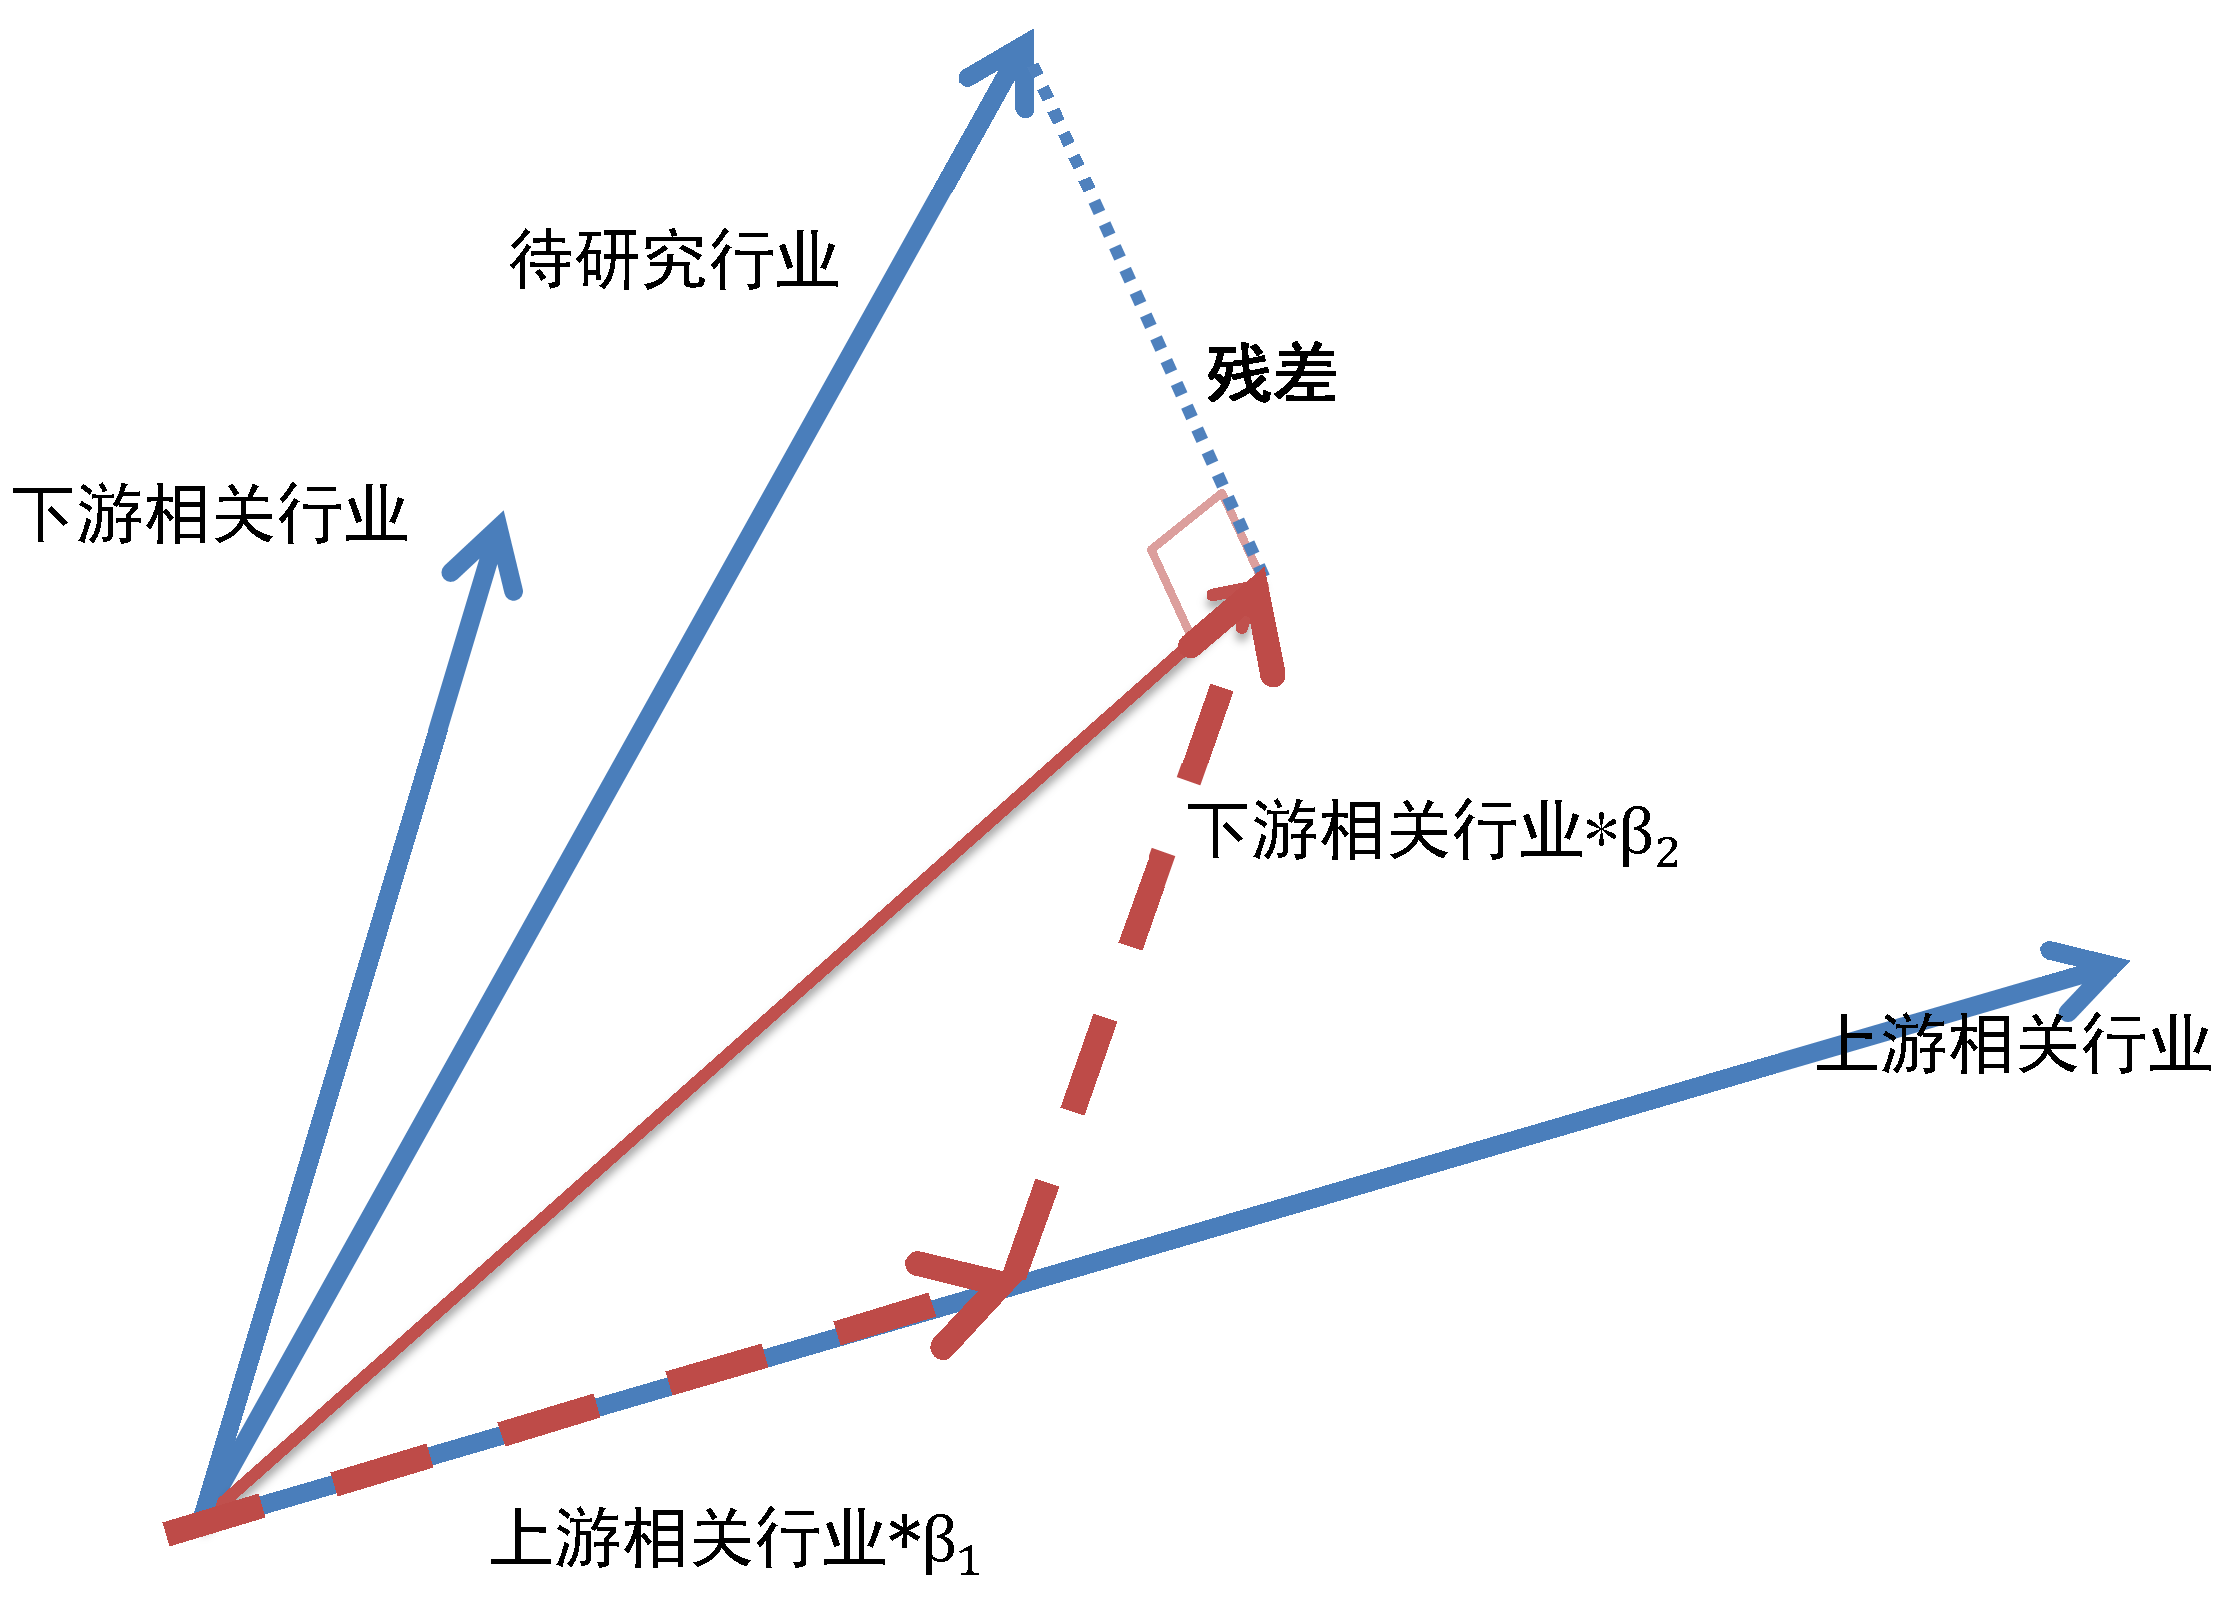
\includegraphics[scale=0.8]{image/最小二乘回归_1_1.png}
\caption{最小二乘估计示意图}
\caption*{\footnotesize 该图从线性代数的角度描述最小二乘回归。其中“待研究行业”是待研究行业到时间t的时间序列,而“上游相关行业”和“下游相关行业”是与待研究行业关联最密切的,经过加权得到的,到时间t-1的时间序列。$\beta_{1}$和$\beta_{2}$分别是这两个时间序列的最小二乘估计系数。}
\label{fig:least-square-estimation}
\end{figure}

投影使得残差尽可能地小,即尽可能地让待研究的行业指数的价格序列被上游和下游的行业指数的价格序列所解释。投影的向量可以表示为上游和下游行业指数价格序列对应的向量的线性组合,得到的系数估计的结果,即最小二乘估计。在给出最小二乘估计前,为了避免时间序列的伪回归问题,我们先对每一个指数的周收益率序列,做序列平稳性的检验。

\subsection{平稳性检验}
在使用最小二乘回归模型前,先检验每个行业指数时间序列的趋势平稳性。若时间序列不存在趋势平稳性时对指数序列进行最小二乘回归,可能出现伪回归。因此,给定每个时间序列,即(\ref{single-ar})式

\begin{equation}
\label{single-ar} 
{\bf {x_t}} = {\bf {c_t}} + \sum\limits_{i = 1}^{p - 1} {{\phi _i}{\bf{x_{t - i}}} + {\bf {e_t}}}
\end{equation}
${\bf {x_t}}$是记录到时间点$t$的序列。${\bf{x_{t - i}}}$是记录到时间点$t-i$前的序列。${\phi _i}$是估计的系数,${\bf {e_t}}$是记录到时间点$t$的残差序列。

检验单位根是否存在,若单位根不存在,则说它是满足趋势平稳的,如果它是趋势平稳的,则可以直接对序列使用最小二乘估计,得到解释变量的系数估计。用ADF(Augmented Dickey-Fuller)检验原假设对备选假设:${H_0}:\beta  = 1\;,\;{H_a}:\beta  < 1$\cite{tsay2013multivariate}。对应的ADF-统计量为:

\begin{equation}
\label{adf-calculation}
ADF - statistic{\rm{ = }}\frac{{\hat \beta {\rm{ - 1}}}}{{s.d.(\hat \beta )}}{\rm{ = }}\frac{{\sum\limits_{t = 1}^T {{\bf{x_{t - 1}}}{\bf {e_t}}} }}{{{\sigma _e}\sqrt {\sum\limits_{t{\rm{ - }}1}^T {\bf{x_{t - 1}^2} }} }}
\end{equation}
式中的${\bf {x_t}}$及${\bf {e_t}}$含义与式\ref{single-ar}相同。

在零假设下,该统计量服从的是自由度为$k-1$的t分布,$k$是样本的个数,且$\hat \sigma _e^{\rm{2}} = \frac{{\sum\limits_{t = 1}^T {{{({x_t} - {{\hat \phi }_1}{x_{t - 1}})}^2}} }}{{T - 1}}$。给定显著性水平,若单位根的原假设被拒绝,则序列存在趋势平稳性。
原假设得到的结果见附录B。由上述结果,在显著性水平$\alpha=0.01$下,绝大部分的指数时间序列拒绝了虚无假设,指数时间序列很有可能满足趋势平稳性。

确保趋势平稳性成立后,以食品加工行业的周收益率序列和周波动率序列为例,给出与其相关的上下游行业的收益率回归系数的最小二乘估计结果,见表\ref{883111-yield-lease-square-estimation}及表\ref{883111-vol-lease-square-estimation}。

\begin{table}[!htbp] \centering 
  \caption{食品加工行业周收益率与上下游行业回归周收益率的系数估计} 
  \caption*{\footnotesize 该表格记录食品加工行业及相关上下游行业的周收益率序列构成的面板数据的最小二乘回归系数估计。第一行和第二行分别是延滞一阶的重组的上游行业指数及重组的下游行业指数的周收益率估计值,第三行是食品加工行业的周收益率序列的估计值,重组时各取5个上游行业和5个下游行业,权重计算见式\ref{yield-weighted}。样本覆盖的时间段为2001年到2016年3月。括号中是各系数估计值的标准差估计值。其中$p$是估计系数为零的零假设为真的概率。显著性记号分别为:{$^{*}$p$<$0.1; $^{**}$p$<$0.05; $^{***}$p$<$0.01}} 
  \label{883111-yield-lease-square-estimation} 
  \renewcommand{\arraystretch}{0.5}
  \begin{tabular}{@{\extracolsep{5pt}}lc} 
  \\[-1.8ex]\hline 
  \hline \\[-1.8ex] 
   & \multicolumn{1}{c}{\textit{因变量:}} \\ 
  \cline{2-2} 
  \\[-1.8ex] & 食品加工行业指数\\ 
  \hline \\[-1.8ex] 
   上游行业指数 & 0.462$^{***}$ \\ 
    & (0.039) \\ 
    & \\ 
   下游行业指数 & 0.293$^{***}$ \\ 
    & (0.043) \\ 
    & \\ 
   截距 & 0.001 \\ 
    & (0.001) \\ 
    & \\ 
  \hline \\[-1.8ex] 
  Observations & 780 \\ 
  R$^{2}$ & 0.726 \\ 
  Adjusted R$^{2}$ & 0.725 \\ 
  Residual Std. Error & 0.022 (df = 777) \\ 
  F Statistic & 1,030.437$^{***}$ (df = 2; 777) \\ 
  \hline 
  \hline \\[-1.8ex] 
  \textit{Note:}  & \multicolumn{1}{r}{$^{*}$p$<$0.1; $^{**}$p$<$0.05; $^{***}$p$<$0.01} \\ 
  \end{tabular} 
\end{table} 

\begin{table}[!htbp] \centering 
  \caption{食品加工行业周波动率与上下游行业周波动率回归的系数估计} 
  \caption*{\footnotesize 该表格记录食品加工行业及相关上下游行业的周波动率序列构成的面板数据的最小二乘回归系数估计。第一行和第二行分别是延滞一阶的重组的上游行业指数及重组的下游行业指数的周波动率估计值,第三行是食品加工行业的周波动率序列的估计值,重组时各取5个上游行业和5个下游行业,权重计算见式\ref{volatility-weighted}。括号中是各系数估计值的标准差估计值。其中$p$是估计系数为零的零假设为真的概率。显著性记号分别为:{$^{*}$p$<$0.1; $^{**}$p$<$0.05; $^{***}$p$<$0.01}} 
  \label{883111-vol-lease-square-estimation} 
  \renewcommand{\arraystretch}{0.5}
  \begin{tabular}{@{\extracolsep{5pt}}lc} 
\\[-1.8ex]\hline 
\hline \\[-1.8ex] 
 & \multicolumn{1}{c}{\textit{因变量:}} \\ 
\cline{2-2} 
\\[-1.8ex] & 食品加工行业指数 \\ 
\hline \\[-1.8ex] 
 上游行业指数 & 0.270$^{***}$ \\ 
  & (0.072) \\ 
  & \\ 
 下游行业指数 & 0.208$^{***}$ \\ 
  & (0.080) \\ 
  & \\ 
 截距 & 0.109$^{***}$ \\ 
  & (0.011) \\ 
  & \\ 
\hline \\[-1.8ex] 
Observations & 732 \\ 
R$^{2}$ & 0.233 \\ 
Adjusted R$^{2}$ & 0.231 \\ 
Residual Std. Error & 0.161 (df = 729) \\ 
F Statistic & 110.770$^{***}$ (df = 2; 729) \\ 
\hline 
\hline \\[-1.8ex] 
\textit{Note:}  & \multicolumn{1}{r}{$^{*}$p$<$0.1; $^{**}$p$<$0.05; $^{***}$p$<$0.01} \\ 
\end{tabular} 
\end{table} 

\section{结果解读与分析}
溢出效应普遍存在于行业指数中。溢出效应存在于收益率序列及波动率序列当中。显著的系数估计表明,市场信息可以沿着行业间的相依关系,进行流动,既而反应在价格上。信息对价格的影响,存在一个逐渐扩散的过程,具体表现为,待研究的行业指数在该时间点的收益率和波动率,相当大的程度上,可以被上一时间点的上游和下游行业指数的收益率和波动率分别解释。这一发现一定程度上挑战了市场有效假说中股价完全反映了市场可得信息的假设。在现实中,投资者的知识面和精力有限,上游和下游行业的信息,需要经过一周左右的时间,才能够完全反映到观测的行业的价格变动上,而且,即使一些投资者提早得知了消息,他们也难以承担短时间内,频繁交易导致的额外的交易成本。这一发现与Hong\cite{hong_industries_2002}及Menzly\cite{menzly_market_2010}在二十世纪六十年代到二十一世纪初的美国股票市场中,产业链关联信息可以逐渐扩散,既而影响股价的过程的发现相吻合。而且,本文发现行业指数间的信息扩散的强度,与行业中具有代表性的个股的信息扩散过程相比较,这一效应强度更大。

溢出效应稳定存在。具体地说,选取样本覆盖区间的子区间再次进行最小二乘回归估计,不影响收益率和波动率同向关联的特点,子样本的结果,可见表\ref{883111-yield-lease-square-estimation-subasample}。这表明,在中国的股票市场,行业间的关联对股价的影响是长期存在的,这一长期存在的基础在于,实体经济网络中的关联是稳定地存在的,并不会因为新的产业的引入,已有产业之间的联系会有剧烈的波动或者变化。然而,根据最小二乘估计的结果,溢出效应往往在一个单位的时间差时,就已经释放。这表现为,将时间差扩展到两个单位时,该时间点往前的第二周,在统计上是不显著的。以波动率的估计结果为例子,见表\ref{883111-vol-lease-square-estimation-second-order}。这一发现与Ahern\cite{ahern2013network}在探究产业信息扩散对股价影响时,关联行业的短期收益率,即前三个月的收益率和长期收益率,即前十二个月到前六个月收益率,都能够解释当前时间点待研究行业的收益率的变化的结论相左。本文认为,结论不一致的原因可能有以下几个因素,第一,研究的对象不同,Ahern选择的是美国在二十世纪九十年代末到二十一世纪初,在美国投入产出表中占比较大,即投入产出值排位在前25\%的行业为研究对象。第二,衡量行业关联的方式不一样,本文采用的是根据流量的强度进行加权的办法,对已有的行业指数进行重新组合,得到重组后的上游行业指数及下游行业指数的收益率及波动率序列,而Ahern是在投入产出表的基础上,纳入了家庭,企业,政府等对象,制作了一个社会收入支出表,再根据这个表格中行业间的流量为研究对象,采用Dyjkstra提出的最短路算法,刻画行业关联的方式,以及冲击扩散的过程。

\begin{table}[!htbp] \centering 
  \caption{食品加工行业周收益率与上下游行业回归周收益率的系数估计} 
  \caption*{\footnotesize 该表格记录食品加工行业及相关上下游行业的周收益率序列构成的面板数据的最小二乘回归系数估计。第一行和第二行分别是延滞一阶的重组的上游行业指数及重组的下游行业指数的周收益率估计值,第三行是食品加工行业的周收益率序列的估计值,重组时各取5个上游行业和5个下游行业,权重计算见式\ref{yield-weighted}。样本覆盖的时间段为2001年到2009年6月。括号中是各系数估计值的标准差估计值。其中$p$是估计系数为零的零假设为真的概率。显著性记号分别为:{$^{*}$p$<$0.1; $^{**}$p$<$0.05; $^{***}$p$<$0.01}} 
  \label{883111-yield-lease-square-estimation-subasample} 
  \renewcommand{\arraystretch}{0.5}
\begin{tabular}{@{\extracolsep{5pt}}lc} 
\\[-1.8ex]\hline 
\hline \\[-1.8ex] 
 & \multicolumn{1}{c}{\textit{因变量:}} \\ 
\cline{2-2} 
\\[-1.8ex] & 食品加工行业指数 \\ 
\hline \\[-1.8ex] 
 上游行业指数 & 0.424$^{***}$ \\ 
  & (0.053) \\ 
  & \\ 
 下游行业指数 & 0.376$^{***}$ \\ 
  & (0.057) \\ 
  & \\ 
 截距 & 0.0005 \\ 
  & (0.001) \\ 
  & \\ 
\hline \\[-1.8ex] 
Observations & 390 \\ 
R$^{2}$ & 0.789 \\ 
Adjusted R$^{2}$ & 0.788 \\ 
Residual Std. Error & 0.021 (df = 387) \\ 
F Statistic & 724.433$^{***}$ (df = 2; 387) \\ 
\hline 
\hline \\[-1.8ex] 
\textit{Note:}  & \multicolumn{1}{r}{$^{*}$p$<$0.1; $^{**}$p$<$0.05; $^{***}$p$<$0.01} \\ 
\end{tabular} 
\end{table} 

\begin{table}[!htbp] \centering 
  \caption{食品加工行业周波动率与上下游行业周波动率回归的系数估计} 
  \caption*{\footnotesize 该表格记录食品加工行业及相关上下游行业的周波动率序列构成的面板数据的最小二乘回归系数估计。第一行和第二行分别是延滞一阶的重组的上游行业指数及重组的下游行业指数的周波动率估计值,第三行和第四行分别是延滞二阶的重组的上游行业指数及重组的下游行业指数的周波动率估计值,第五行是食品加工行业的周波动率序列截距的估计值,重组时各取5个上游行业和5个下游行业,权重计算见式\ref{volatility-weighted}。括号中是各系数估计值的标准差估计值。其中$p$是估计系数为零的零假设为真的概率。显著性记号分别为:{$^{*}$p$<$0.1; $^{**}$p$<$0.05; $^{***}$p$<$0.01}} 
  \label{883111-vol-lease-square-estimation-second-order} 
  \renewcommand{\arraystretch}{0.5}
\begin{tabular}{@{\extracolsep{5pt}}lc} 
\\[-1.8ex]\hline 
\hline \\[-1.8ex] 
 & \multicolumn{1}{c}{\textit{因变量:}} \\ 
\cline{2-2} 
\\[-1.8ex] & 食品加工行业指数 \\ 
\hline \\[-1.8ex] 
 上游行业延滞一阶 & 0.207$^{***}$ \\ 
  & (0.072) \\ 
  & \\ 
 上游行业延滞二阶 & 0.117 \\ 
  & (0.073) \\ 
  & \\ 
 下游行业延滞一阶 & 0.164$^{**}$ \\ 
  & (0.079) \\ 
  & \\ 
 下游行业延滞二阶 & 0.136$^{*}$ \\ 
  & (0.080) \\ 
  & \\ 
 截距 & 0.069$^{***}$ \\ 
  & (0.012) \\ 
  & \\ 
\hline \\[-1.8ex] 
Observations & 708 \\ 
R$^{2}$ & 0.291 \\ 
Adjusted R$^{2}$ & 0.287 \\ 
Residual Std. Error & 0.156 (df = 703) \\ 
F Statistic & 71.980$^{***}$ (df = 4; 703) \\ 
\hline 
\hline \\[-1.8ex] 
\textit{Note:}  & \multicolumn{1}{r}{$^{*}$p$<$0.1; $^{**}$p$<$0.05; $^{***}$p$<$0.01} \\ 
\end{tabular} 
\end{table} 

溢出效应的强度,取决于行业自身的特征。以食品加工行业为例,在研究的时间段内,它在该时间点的收益率和波动率,均与加权的上游行业指数和下游行业指数正向地相关。然而,对于农业,在研究的时间段内,它在该时间点的收益率和波动率,与加权的上游行业指数负向相关,但与加权的下游行业指数正向相关。更具体地说,下游行业和上游行业的影响存在差异。

\section{参数敏感性分析}

考虑行业数目的变化,对模型参数估计的影响。本文尝试了关联行业为3个行业,5个行业和10个行业的情形,重新估计模型中各变元的参数,取10个行业的估计的结果为例,见表。由估计的结果可见,行业间收益率序列,仍然存在溢出的效应,而且,上游和下游行业的周收益率和周波动率序列解释能力依然保持。

\begin{table}[!htbp] \centering 
  \caption{食品加工行业周收益率与上下游行业回归周收益率的系数估计} 
  \caption*{\footnotesize 该表格记录食品加工行业及相关上下游行业的周收益率序列构成的面板数据的最小二乘回归系数估计。第一行和第二行分别是延滞一阶的重组的上游行业指数及重组的下游行业指数的周收益率序列估计值,第三行是食品加工行业的周收益率序列的估计值,重组时各取10个上游行业和10个下游行业,权重计算见式\ref{yield-weighted}。样本覆盖的时间段为2001年到2016年3月。括号中是各系数估计值的标准差估计值。其中$p$是估计系数为零的零假设为真的概率。显著性记号分别为:{$^{*}$p$<$0.1; $^{**}$p$<$0.05; $^{***}$p$<$0.01}} 
  \label{883111-yield-lease-square-estimation-10sectors} 
  \renewcommand{\arraystretch}{0.5}

\begin{tabular}{@{\extracolsep{5pt}}lc} 
\\[-1.8ex]\hline 
\hline \\[-1.8ex] 
 & \multicolumn{1}{c}{\textit{因变量:}} \\ 
\cline{2-2} 
\\[-1.8ex] & 食品加工行业指数 \\ 
\hline \\[-1.8ex] 
 上游行业指数 & 0.429$^{***}$ \\ 
  & (0.043) \\ 
  & \\ 
 下游行业指数 & 0.352$^{***}$ \\ 
  & (0.046) \\ 
  & \\ 
 截距 & 0.0005 \\ 
  & (0.001) \\ 
  & \\ 
\hline \\[-1.8ex] 
Observations & 780 \\ 
R$^{2}$ & 0.740 \\ 
Adjusted R$^{2}$ & 0.739 \\ 
Residual Std. Error & 0.022 (df = 777) \\ 
F Statistic & 1,104.407$^{***}$ (df = 2; 777) \\ 
\hline 
\hline \\[-1.8ex] 
\textit{Note:}  & \multicolumn{1}{r}{$^{*}$p$<$0.1; $^{**}$p$<$0.05; $^{***}$p$<$0.01} \\ 
\end{tabular} 
\end{table} 

\begin{table}[!htbp] \centering 
  \caption{食品加工行业周波动率与上下游行业周波动率回归的系数估计} 
  \caption*{\footnotesize 该表格记录食品加工行业及相关上下游行业的周波动率序列构成的面板数据的最小二乘回归系数估计。第一行和第二行分别是延滞一阶的重组的上游行业指数及重组的下游行业指数的周波动率序列估计值,第三行是食品加工行业的周波动率序列的估计值,重组时各取10个上游行业和10个下游行业,权重计算见式\ref{volatility-weighted}。括号中是各系数估计值的标准差估计值。其中$p$是估计系数为零的零假设为真的概率。显著性记号分别为:{$^{*}$p$<$0.1; $^{**}$p$<$0.05; $^{***}$p$<$0.01}} 
  \label{883111-vol-lease-square-estimation-10sectors} 
  \renewcommand{\arraystretch}{0.5}
 \begin{tabular}{@{\extracolsep{5pt}}lc} 
\\[-1.8ex]\hline 
\hline \\[-1.8ex] 
 & \multicolumn{1}{c}{\textit{因变量:}} \\ 
\cline{2-2} 
\\[-1.8ex] & 食品加工行业指数 \\ 
\hline \\[-1.8ex] 
 上游行业指数 & 0.268$^{***}$ \\ 
  & (0.080) \\ 
  & \\ 
 下游行业指数 & 0.216$^{**}$ \\ 
  & (0.088) \\ 
  & \\ 
 截距 & 0.110$^{***}$ \\ 
  & (0.011) \\ 
  & \\ 
\hline \\[-1.8ex] 
Observations & 732 \\ 
R$^{2}$ & 0.231 \\ 
Adjusted R$^{2}$ & 0.229 \\ 
Residual Std. Error & 0.161 (df = 729) \\ 
F Statistic & 109.585$^{***}$ (df = 2; 729) \\ 
\hline 
\hline \\[-1.8ex] 
\textit{Note:}  & \multicolumn{1}{r}{$^{*}$p$<$0.1; $^{**}$p$<$0.05; $^{***}$p$<$0.01} \\ 
\end{tabular} 
\end{table} 

\chapter{结束语}

\section{主要研究结论}

溢出效应在行业指数间普遍存在。具体表现为,待研究行业的在该时间点的收益率和波动率,很大程度上被下游行业和上游行业在前一周的收益率和波动率所解释。这一现象表明,影响股价的信号,可以沿着产业链,从上游产业对应的上市公司及下游产业对应的上市公司,传导到待研究行业。这一现象在指定行业后,并不随着关联行业的数目的改变而有显著的变化。

\section{研究局限性}

本文没有对不同信息产生的效应作区分。信息的异质性对模型的解释力有很重要的影响。具体表现为,一方面,投资者对正面和负面的信息的反应有所差别,另一方面,市场中投资者对同一信息有不同的响应。例如,风险厌恶者往往会对负面的信息作更剧烈的反应。于此同时,由于篇幅所限,并没有作进一步的探讨。这可以作为进一步探究的方向。

本文没有结合行业内部和行业间的变量探究溢出效应。在实际投资决策的过程中,行业间的变量的信息与行业外部的变量是需要同时纳入考量的。然而,行业内部变量的获取,受到数据可得性及数据处理能力的制约,没有纳入本文的讨论范围。

\zihao{-5}\songti
\bibliographystyle{sysuthesis}
\bibliography{我的文献库,main}%假定bib文件为main.bib
\appendix

\begin{thankto}

\songti\zihao{-4}

我要感谢毕业论文书写过程中给予我指导和殷切关怀的老师。老师们严谨的治学态度和严格的要求,让我丝毫不敢放松对学术论文写作的要求,这为我将来作进一步的学习和研究,打下了坚实的基础。老师们对解决问题的热忱,以及发现新方向的敏锐目光,一次次地让我在将要迷失方向的时候,为我点出解决问题的方向。我要特别感谢指导我毕业论文的刘老师和曾老师,他们在我毕业论文选题及书写的过程中,与我进行了深入的探讨和交流,让我可以接触到前沿的研究问题,更难能可贵的是,他们的一言一行,无时无刻不启发我结合自身的优势和特点,寻找感兴趣的问题,并尝试深入其中,努力钻研。在汇报研究的进展时,两位老师都给予了我富有建设性的建议,你们的指导我永远铭记在心。

我还要感谢我的父母,他们对我的学习和生活非常关切。在论文书写的过程中,家人的关心和支持给我提供了长足的动力,也激励我更努力地突破自己的极限,努力活出新的高度。虽然,有限的成果难以回报你们对我无限的关爱,但我会继续努力,争取用更好的成绩,更优秀的我,回报你们,不辜负你们的期待。

\vskip 18pt
\begin{flushright}
李俊成\\
\today
\end{flushright}
\end{thankto}

%接下来是附录部分,以\chapter{附录标题}开始一个新的附录
\chapter{数据来源,数据处理及输出结果说明}
将数据分为三类,原始输入数据,中间处理数据,输出结果。原始输入数据包括2002年,2007年及2012年的中国国民经济投入产出表的中间投入部分,分别对应2002-123-raw.csv,2007-129-raw.csv,2012-139-raw.csv文件。以及WIND资讯中提取的证监会行业指数,包括自指数编制以来,每个交易日的开盘价,收盘价,涨幅和跌幅,对应文件是Wind-证监会指数-完整版.csv。
证监会的行业分类与投入产出表的分类存在一些差异,这些差异主要体现在三个方面。一:一部分的行业在证券市场中没有上市公司,例如公益服务业,政府机构。二:有一部分的行业指数,一个指数包含多个子行业。三:由于行业分类标准在2011年发生了变动,因此,2007年及2002年的投入产出表中,有一部分指数对应的行业是当时没有细分的。为了克服差异造成统计上的不便,我们额外制作了三个表格,每个表格都建立了当年投入产出表中各行业与证监会行业指数的对应关系。接着,我们按照表\ref{fig:iomapping},将投入产出表各行业中的流量,转化为各行业指数对应实体经济的流量表\ref{fig:reorganized-ioaccount}。具体的转换操作可见源程序Raw-To-CC-Re.R,输出的流量矩阵对应的文件是Flow12-Re.csv,Flow07-Re.csv,Flow02-Re.csv。
接着,计算各个行业的收益率序列。我们先从月收益率序列开始,月收益率计算的方式是t月的指数价格,除于t-1月的指数的价格,再取对数。得到了月收益率序列后,将它存在文件monthyield-zoo-series.csv中。
转换完成后,则可以开始对行业的上游和下游行业作分析。对行业矩阵的列向量,取各列的前k个对应的行业,记为每个行业的上游行业的收益率序列。类似地,对流量矩阵的行向量,取各行前k个对应的行业,记为每个行业的下游行业的收益率序列。为了测试交叉预测性,对上游行业和下游行业的序列作一个单位的时延,将时延后得到的上下游收益率序列与行业收益率序列作组合,得到一个面板数据。再对这个面板数据作最小二乘回归。

\chapter{行业指数平稳性检验结果}
\begin{table}[htbp]
  \centering
  \label{stationaryofseries}
  \caption{收益列序列平稳性检验}
  \caption*{\footnotesize 该表格是不同行业的收益率序列的平稳性检验的估计,第一列是各个行业指数的代号,第二列是统计量的估计值,第三列是在1\%的显著性水平下,检验的零假设的阈值,第三列是判断估计值的绝对值是否超过阈值,若超过则记为1,反之记为0.} 
    \scalebox{0.5}{
     \renewcommand{\arraystretch}{0.5}%
    \begin{tabular}{rrrrrrrrrrrr}
          & out   & thres & stationary &       & out   & thres & stationary &       & out   & thres & stationary \\

    883023.WI & -5.423863492 & -3.99 & 1     & 883131.WI & -4.734046849 & -3.99 & 1     & 883159.WI & -5.159013964 & -3.99 & 1 \\
    883023.WI & 9.898247604 & 6.22  & 1     & 883131.WI & 7.589502562 & 6.22  & 1     & 883159.WI & 8.946579114 & 6.22  & 1 \\
    883023.WI & 14.7824398 & 8.43  & 1     & 883131.WI & 11.29828702 & 8.43  & 1     & 883159.WI & 13.36423372 & 8.43  & 1 \\
    883028.WI & -5.076156918 & -3.99 & 1     & 883132.WI & -5.038095733 & -3.99 & 1     & 883160.WI & -5.085544315 & -3.99 & 1 \\
    883028.WI & 8.696173147 & 6.22  & 1     & 883132.WI & 8.56459587 & 6.22  & 1     & 883160.WI & 8.706684778 & 6.22  & 1 \\
    883028.WI & 12.95482807 & 8.43  & 1     & 883132.WI & 12.7660432 & 8.43  & 1     & 883160.WI & 12.9908107 & 8.43  & 1 \\
    883111.WI & -5.40156254 & -3.99 & 1     & 883133.WI & -5.195448332 & -3.99 & 1     & 883161.WI & -5.531202903 & -3.99 & 1 \\
    883111.WI & 9.79169621 & 6.22  & 1     & 883133.WI & 9.06485028 & 6.22  & 1     & 883161.WI & 10.21532833 & 6.22  & 1 \\
    883111.WI & 14.63733766 & 8.43  & 1     & 883133.WI & 13.53364823 & 8.43  & 1     & 883161.WI & 15.30108611 & 8.43  & 1 \\
    883112.WI & -5.304964252 & -3.99 & 1     & 883134.WI & -5.466540779 & -3.99 & 1     & 883162.WI & -5.666808093 & -3.99 & 1 \\
    883112.WI & 9.428695224 & 6.22  & 1     & 883134.WI & 10.04159129 & 6.22  & 1     & 883162.WI & 10.73502117 & 6.22  & 1 \\
    883112.WI & 14.08990091 & 8.43  & 1     & 883134.WI & 15.00024324 & 8.43  & 1     & 883162.WI & 16.09441806 & 8.43  & 1 \\
    883113.WI & -5.970474504 & -3.99 & 1     & 883135.WI & -5.036370897 & -3.99 & 1     & 883164.WI & -5.54077089 & -3.99 & 1 \\
    883113.WI & 11.9099471 & 6.22  & 1     & 883135.WI & 8.569695896 & 6.22  & 1     & 883164.WI & 10.26846802 & 6.22  & 1 \\
    883113.WI & 17.82803648 & 8.43  & 1     & 883135.WI & 12.76811438 & 8.43  & 1     & 883164.WI & 15.36295164 & 8.43  & 1 \\
    883114.WI & -4.854610092 & -3.99 & 1     & 883136.WI & -5.274682134 & -3.99 & 1     & 883165.WI & -5.64046973 & -3.99 & 1 \\
    883114.WI & 7.913672532 & 6.22  & 1     & 883136.WI & 9.372135095 & 6.22  & 1     & 883165.WI & 10.67903634 & 6.22  & 1 \\
    883114.WI & 11.82160285 & 8.43  & 1     & 883136.WI & 13.98036231 & 8.43  & 1     & 883165.WI & 15.96906835 & 8.43  & 1 \\
    883115.WI & -5.712631978 & -3.99 & 1     & 883137.WI & -4.638125072 & -3.99 & 1     & 883166.WI & -4.914724327 & -3.99 & 1 \\
    883115.WI & 10.92768837 & 6.22  & 1     & 883137.WI & 7.251867616 & 6.22  & 1     & 883166.WI & 8.059914646 & 6.22  & 1 \\
    883115.WI & 16.34990046 & 8.43  & 1     & 883137.WI & 10.80134392 & 8.43  & 1     & 883166.WI & 12.07734491 & 8.43  & 1 \\
    883116.WI & -5.233418348 & -3.99 & 1     & 883138.WI & -5.94660057 & -3.99 & 1     & 883167.WI & -5.411601449 & -3.99 & 1 \\
    883116.WI & 9.215016431 & 6.22  & 1     & 883138.WI & 11.83923889 & 6.22  & 1     & 883167.WI & 9.839053815 & 6.22  & 1 \\
    883116.WI & 13.79899104 & 8.43  & 1     & 883138.WI & 17.71515533 & 8.43  & 1     & 883167.WI & 14.69123338 & 8.43  & 1 \\
    883117.WI & -4.975274834 & -3.99 & 1     & 883139.WI & -4.662666307 & -3.99 & 1     & 883169.WI & -4.59950239 & -3.99 & 1 \\
    883117.WI & 8.411280964 & 6.22  & 1     & 883139.WI & 7.28147156 & 6.22  & 1     & 883169.WI & 7.208121814 & 6.22  & 1 \\
    883117.WI & 12.58332498 & 8.43  & 1     & 883139.WI & 10.88239641 & 8.43  & 1     & 883169.WI & 10.70615744 & 8.43  & 1 \\
    883118.WI & -4.457292873 & -3.99 & 1     & 883140.WI & -4.452812875 & -3.99 & 1     & 883170.WI & -5.930688269 & -3.99 & 1 \\
    883118.WI & 6.679621299 & 6.22  & 1     & 883140.WI & 6.655788341 & 6.22  & 1     & 883170.WI & 11.73937283 & 6.22  & 1 \\
    883118.WI & 9.960587121 & 8.43  & 1     & 883140.WI & 9.92877838 & 8.43  & 1     & 883170.WI & 17.60556292 & 8.43  & 1 \\
    883119.WI & -4.688665079 & -3.99 & 1     & 883141.WI & -4.933195033 & -3.99 & 1     & 883172.WI & -8.611537589 & -3.99 & 1 \\
    883119.WI & 7.409411802 & 6.22  & 1     & 883141.WI & 8.129593753 & 6.22  & 1     & 883172.WI & 24.7207698 & 6.22  & 1 \\
    883119.WI & 11.05241291 & 8.43  & 1     & 883141.WI & 12.168864 & 8.43  & 1     & 883172.WI & 37.08072124 & 8.43  & 1 \\
    883120.WI & -5.422675661 & -3.99 & 1     & 883142.WI & -5.407869589 & -3.99 & 1     & 883175.WI & -5.954368579 & -3.99 & 1 \\
    883120.WI & 9.836631552 & 6.22  & 1     & 883142.WI & 9.827594033 & 6.22  & 1     & 883175.WI & 11.82975641 & 6.22  & 1 \\
    883120.WI & 14.72217263 & 8.43  & 1     & 883142.WI & 14.68282524 & 8.43  & 1     & 883175.WI & 17.73510534 & 8.43  & 1 \\
    883121.WI & -3.548147911 & -3.99 & 0     & 883143.WI & -5.084230628 & -3.99 & 1     & 883176.WI & -5.257807029 & -3.99 & 1 \\
    883121.WI & 4.581888254 & 6.22  & 0     & 883143.WI & 8.63687205 & 6.22  & 1     & 883176.WI & 9.315469954 & 6.22  & 1 \\
    883121.WI & 6.677224806 & 8.43  & 0     & 883143.WI & 12.92766384 & 8.43  & 1     & 883176.WI & 13.8975674 & 8.43  & 1 \\
    883122.WI & -5.194307235 & -3.99 & 1     & 883144.WI & -5.792464466 & -3.99 & 1     & 883177.WI & -4.977364278 & -3.99 & 1 \\
    883122.WI & 9.107411675 & 6.22  & 1     & 883144.WI & 11.33703752 & 6.22  & 1     & 883177.WI & 8.405139994 & 6.22  & 1 \\
    883122.WI & 13.57669261 & 8.43  & 1     & 883144.WI & 16.89675332 & 8.43  & 1     & 883177.WI & 12.49967873 & 8.43  & 1 \\
    883123.WI & -5.414044272 & -3.99 & 1     & 883145.WI & -6.548772371 & -3.99 & 1     & 883178.WI & -9.158736831 & -3.99 & 1 \\
    883123.WI & 9.870599032 & 6.22  & 1     & 883145.WI & 14.3021667 & 6.22  & 1     & 883178.WI & 27.96133583 & 6.22  & 1 \\
    883123.WI & 14.73439138 & 8.43  & 1     & 883145.WI & 21.44494776 & 8.43  & 1     & 883178.WI & 41.94126675 & 8.43  & 1 \\
    883124.WI & -5.590582697 & -3.99 & 1     & 883146.WI & -5.457615223 & -3.99 & 1     & 883180.WI & -6.72804419 & -3.99 & 1 \\
    883124.WI & 10.4986514 & 6.22  & 1     & 883146.WI & 10.08091094 & 6.22  & 1     & 883180.WI & 15.09945178 & 6.22  & 1 \\
    883124.WI & 15.68480716 & 8.43  & 1     & 883146.WI & 15.02153292 & 8.43  & 1     & 883180.WI & 22.63331881 & 8.43  & 1 \\
    883125.WI & -4.698235501 & -3.99 & 1     & 883147.WI & -6.090704456 & -3.99 & 1     & 883181.WI & -5.580461136 & -3.99 & 1 \\
    883125.WI & 7.421652748 & 6.22  & 1     & 883147.WI & 12.40669948 & 6.22  & 1     & 883181.WI & 10.42831831 & 6.22  & 1 \\
    883125.WI & 11.07703682 & 8.43  & 1     & 883147.WI & 18.59995536 & 8.43  & 1     & 883181.WI & 15.59740912 & 8.43  & 1 \\
    883126.WI & -5.044102738 & -3.99 & 1     & 883148.WI & -8.904805181 & -3.99 & 1     & 883182.WI & -5.07040254 & -3.99 & 1 \\
    883126.WI & 8.562307653 & 6.22  & 1     & 883148.WI & 26.4323308 & 6.22  & 1     & 883182.WI & 8.678920165 & 6.22  & 1 \\
    883126.WI & 12.77985518 & 8.43  & 1     & 883148.WI & 39.64779603 & 8.43  & 1     & 883182.WI & 12.92834492 & 8.43  & 1 \\
    883127.WI & -5.278930456 & -3.99 & 1     & 883149.WI & -5.477858239 & -3.99 & 1     & 883183.WI & -5.705086286 & -3.99 & 1 \\
    883127.WI & 9.377373458 & 6.22  & 1     & 883149.WI & 10.04224252 & 6.22  & 1     & 883183.WI & 10.86019685 & 6.22  & 1 \\
    883127.WI & 13.99274225 & 8.43  & 1     & 883149.WI & 15.03125352 & 8.43  & 1     & 883183.WI & 16.27552677 & 8.43  & 1 \\
    883128.WI & -4.823067946 & -3.99 & 1     & 883150.WI & -4.897311638 & -3.99 & 1     & 883186.WI & -5.785523414 & -3.99 & 1 \\
    883128.WI & 7.921483029 & 6.22  & 1     & 883150.WI & 8.03402152 & 6.22  & 1     & 883186.WI & 11.18815615 & 6.22  & 1 \\
    883128.WI & 11.76713115 & 8.43  & 1     & 883150.WI & 12.01321275 & 8.43  & 1     & 883186.WI & 16.74399574 & 8.43  & 1 \\
    883129.WI & -5.369293682 & -3.99 & 1     & 883151.WI & -4.988699883 & -3.99 & 1     & 883187.WI & -3.969586873 & -3.99 & 0 \\
    883129.WI & 9.662575658 & 6.22  & 1     & 883151.WI & 8.325861699 & 6.22  & 1     & 883187.WI & 5.471823801 & 6.22  & 0 \\
    883129.WI & 14.43808103 & 8.43  & 1     & 883151.WI & 12.45416911 & 8.43  & 1     & 883187.WI & 8.081194188 & 8.43  & 0 \\
    883130.WI & -4.967095828 & -3.99 & 1     & 883158.WI & -6.053028218 & -3.99 & 1     & 883189.WI & -8.452016676 & -3.99 & 1 \\
    883130.WI & 8.314289875 & 6.22  & 1     & 883158.WI & 12.22322003 & 6.22  & 1     & 883189.WI & 23.825685 & 6.22  & 1 \\
    883130.WI & 12.39720682 & 8.43  & 1     & 883158.WI & 18.31978275 & 8.43  & 1     & 883189.WI & 35.72632892 & 8.43  & 1 \\

    \end{tabular}
    }
\end{table}

\chapter{食品加工行业指数的周收益率及周波动率折线图-同期叠加部分}

同期叠加部分的图与分列图表分开列出,是为了呈现论文核心研究的同时,尽可能地避免连续过多的图片对读者造成困扰,因此,将同期叠加部分放在附表中,供感兴趣的读者进一步查阅。

\begin{figure}[htbp]
\centering
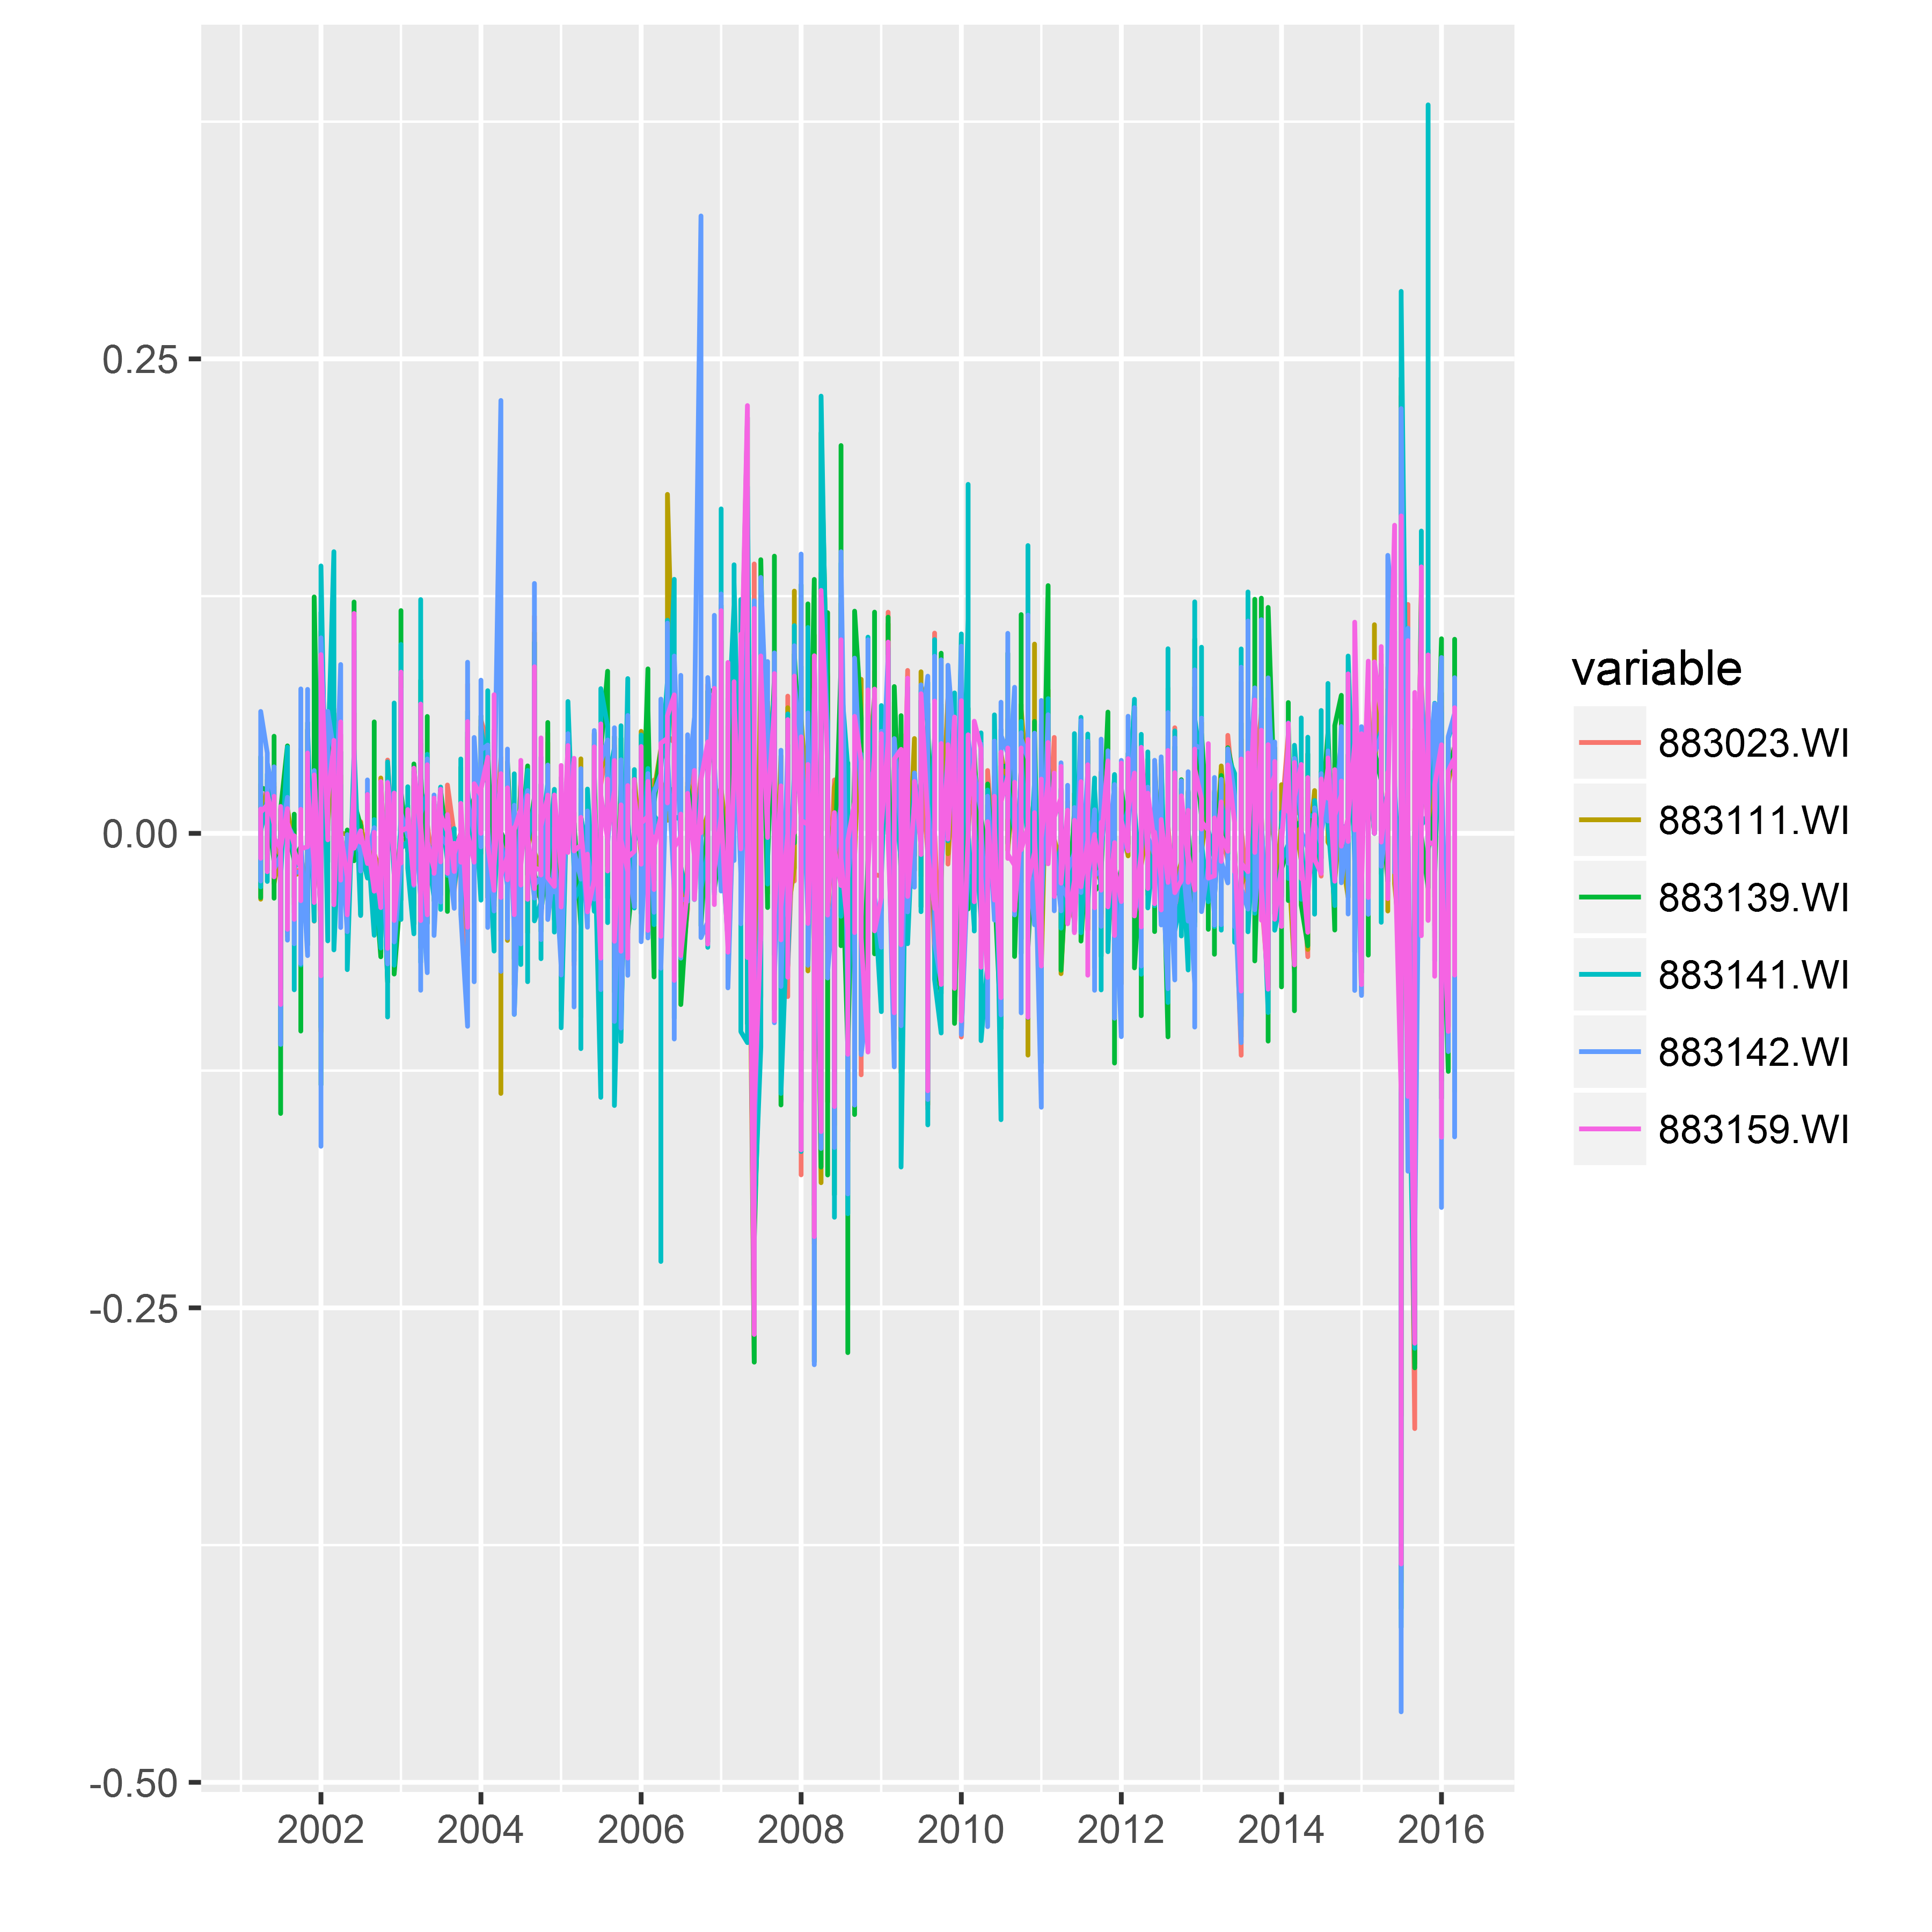
\includegraphics[scale=0.8]{image/883111-topk-upper-plus-one-weeklyyield-combined.png}
\caption{食品加工行业指数与关联最密切的五个上游行业指数的周收益率序列-指数同期叠加}
\caption*{\footnotesize 该图记录了食品加工行业指数与关联最密切的五个上游行业指数的周收益率的折线图,$X$轴是时间,从2001年4月第一周开始,到2016年3月最后一周。$Y$轴是对数周收益率。每种颜色代表一个行业指数的收益率序列。}
\label{fig:883111-topk-upper-plus-one-weeklyyield-combined}
\end{figure}

\begin{figure}[htbp]
\centering
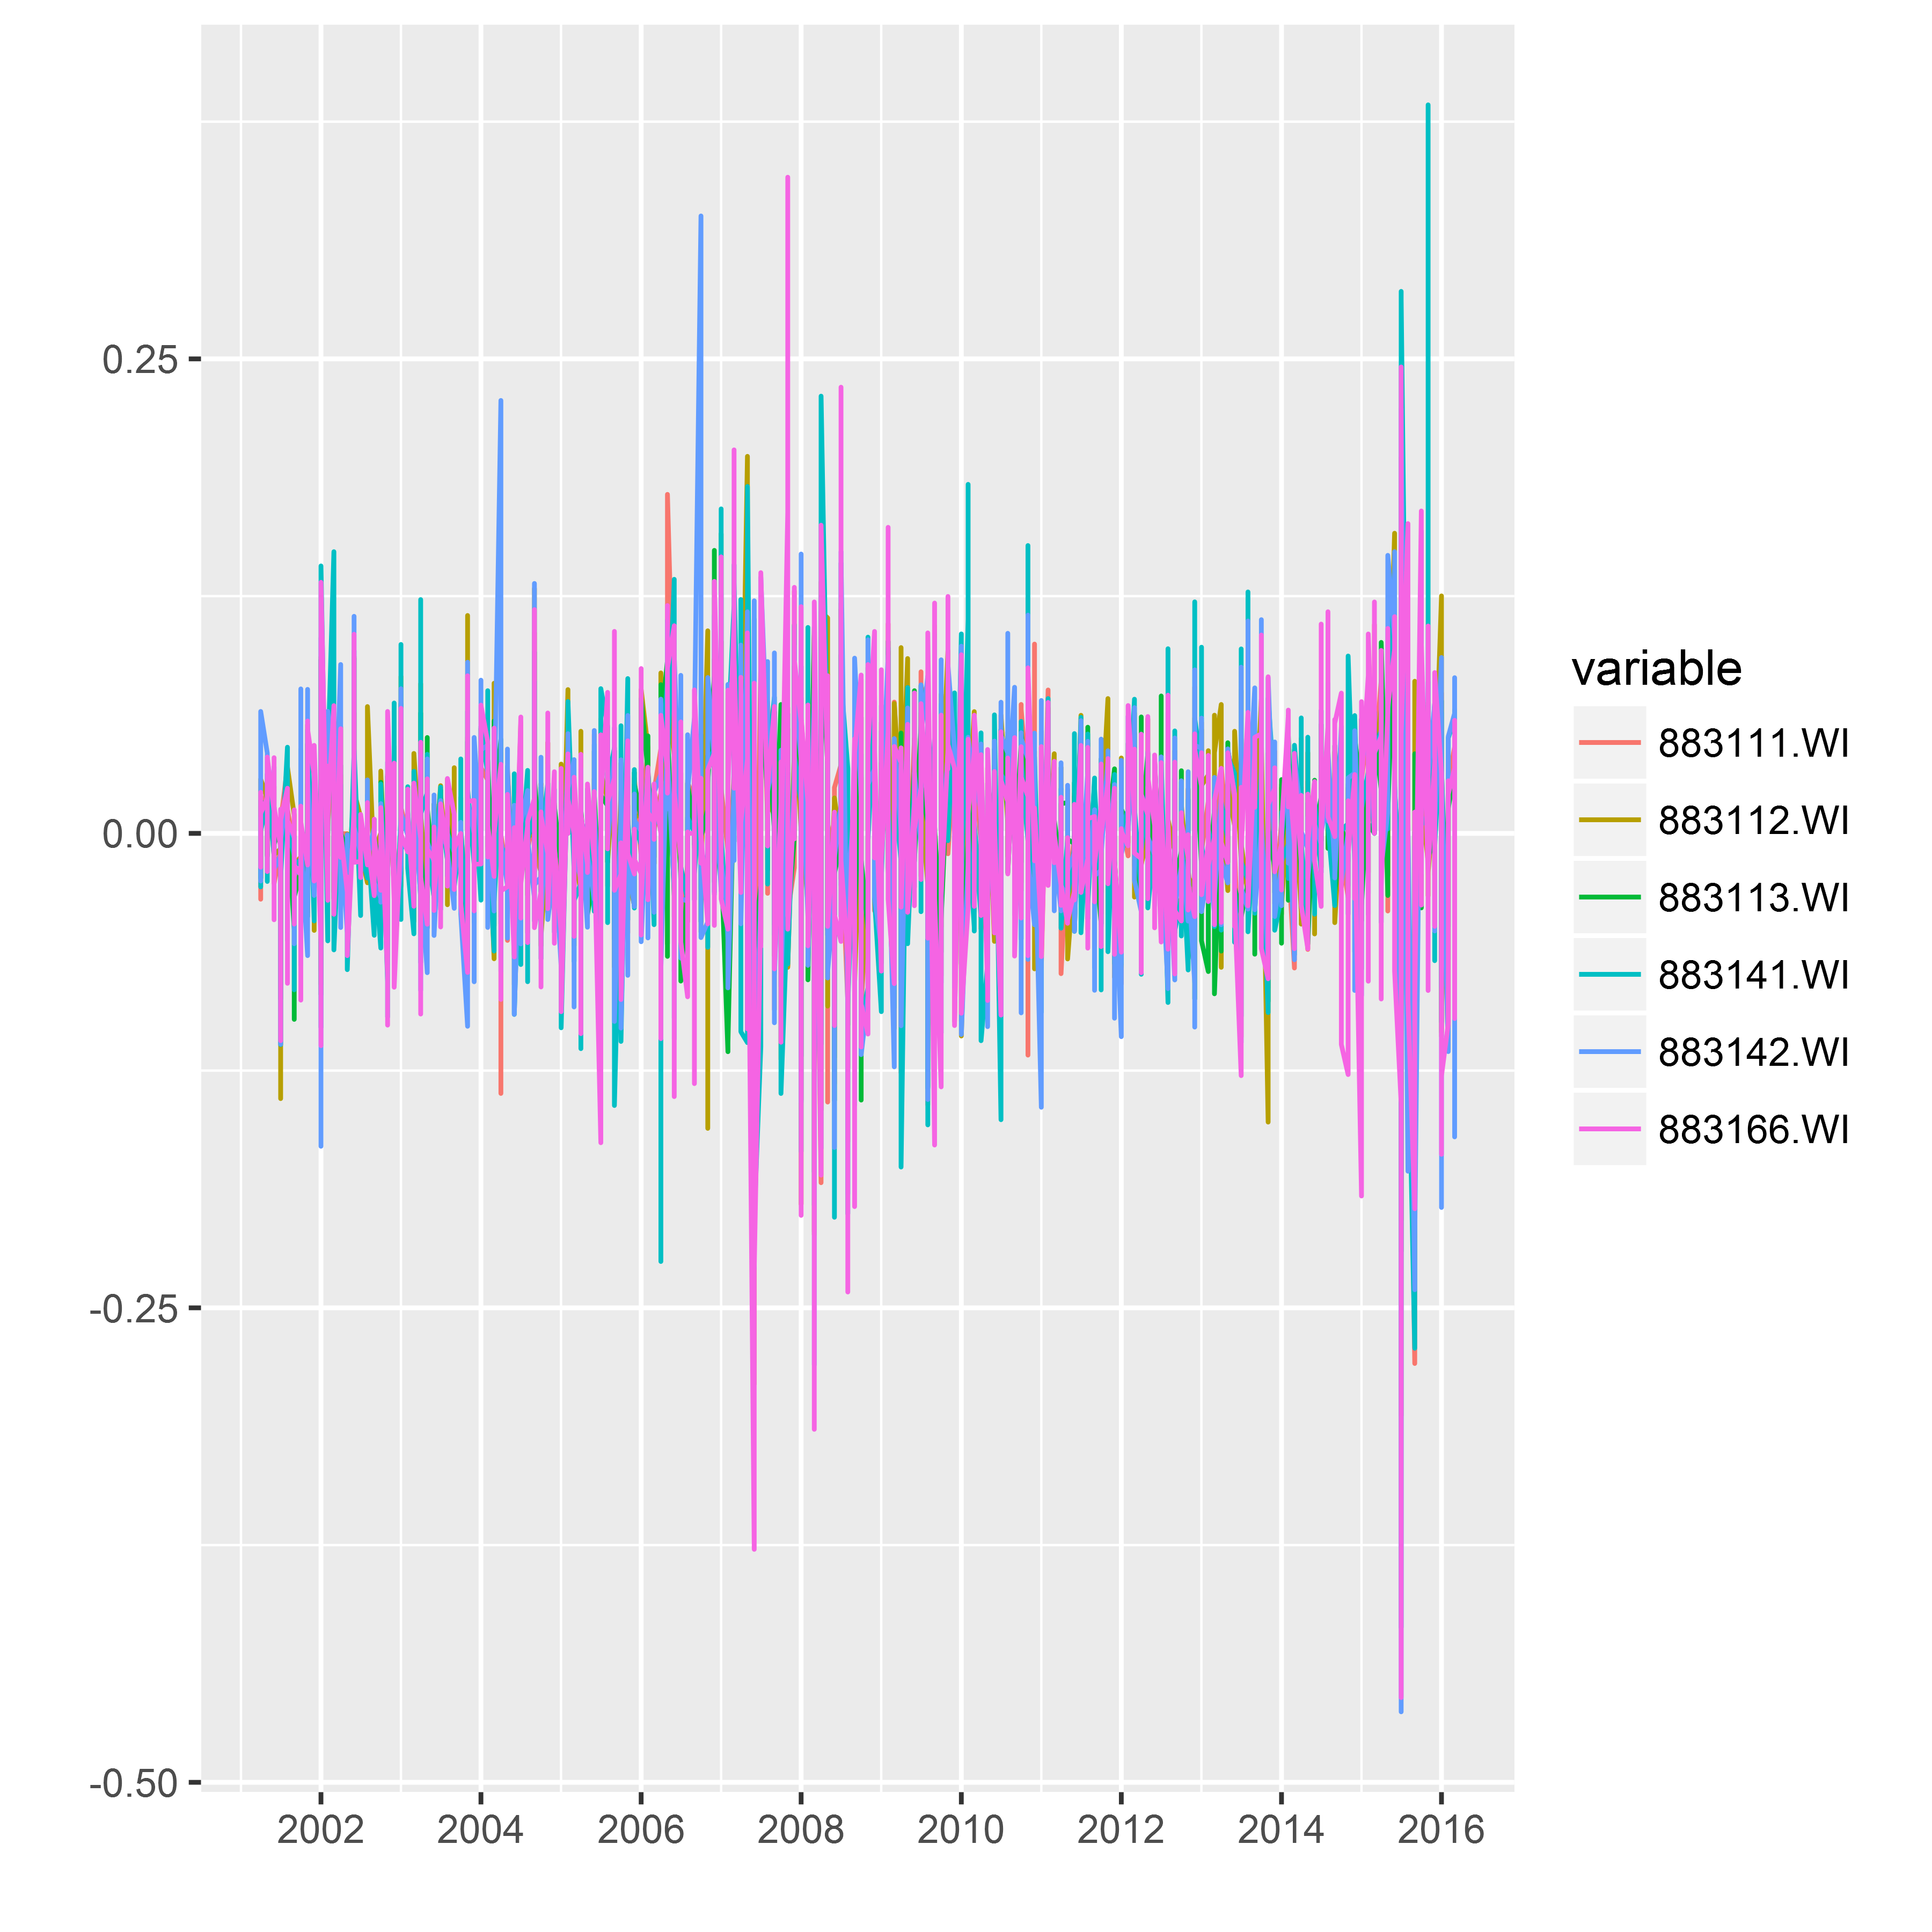
\includegraphics[scale=0.8]{image/883111-topk-lower-plus-one-weeklyyield-combined.png}
\caption{食品加工行业指数与关联最密切的五个下游行业指数的周收益率序列-指数同期叠加}
\caption*{\footnotesize 该图记录了食品加工行业指数与关联最密切的五个下游行业指数的周收益率的折线图,$X$轴是时间,从2001年4月第一周开始,到2016年3月最后一周。$Y$轴是对数周收益率。每种颜色代表一个行业指数的收益率序列。}
\label{fig:883111-topk-lower-plus-one-weeklyyield-combined}
\end{figure}

\begin{figure}[htbp]
\centering
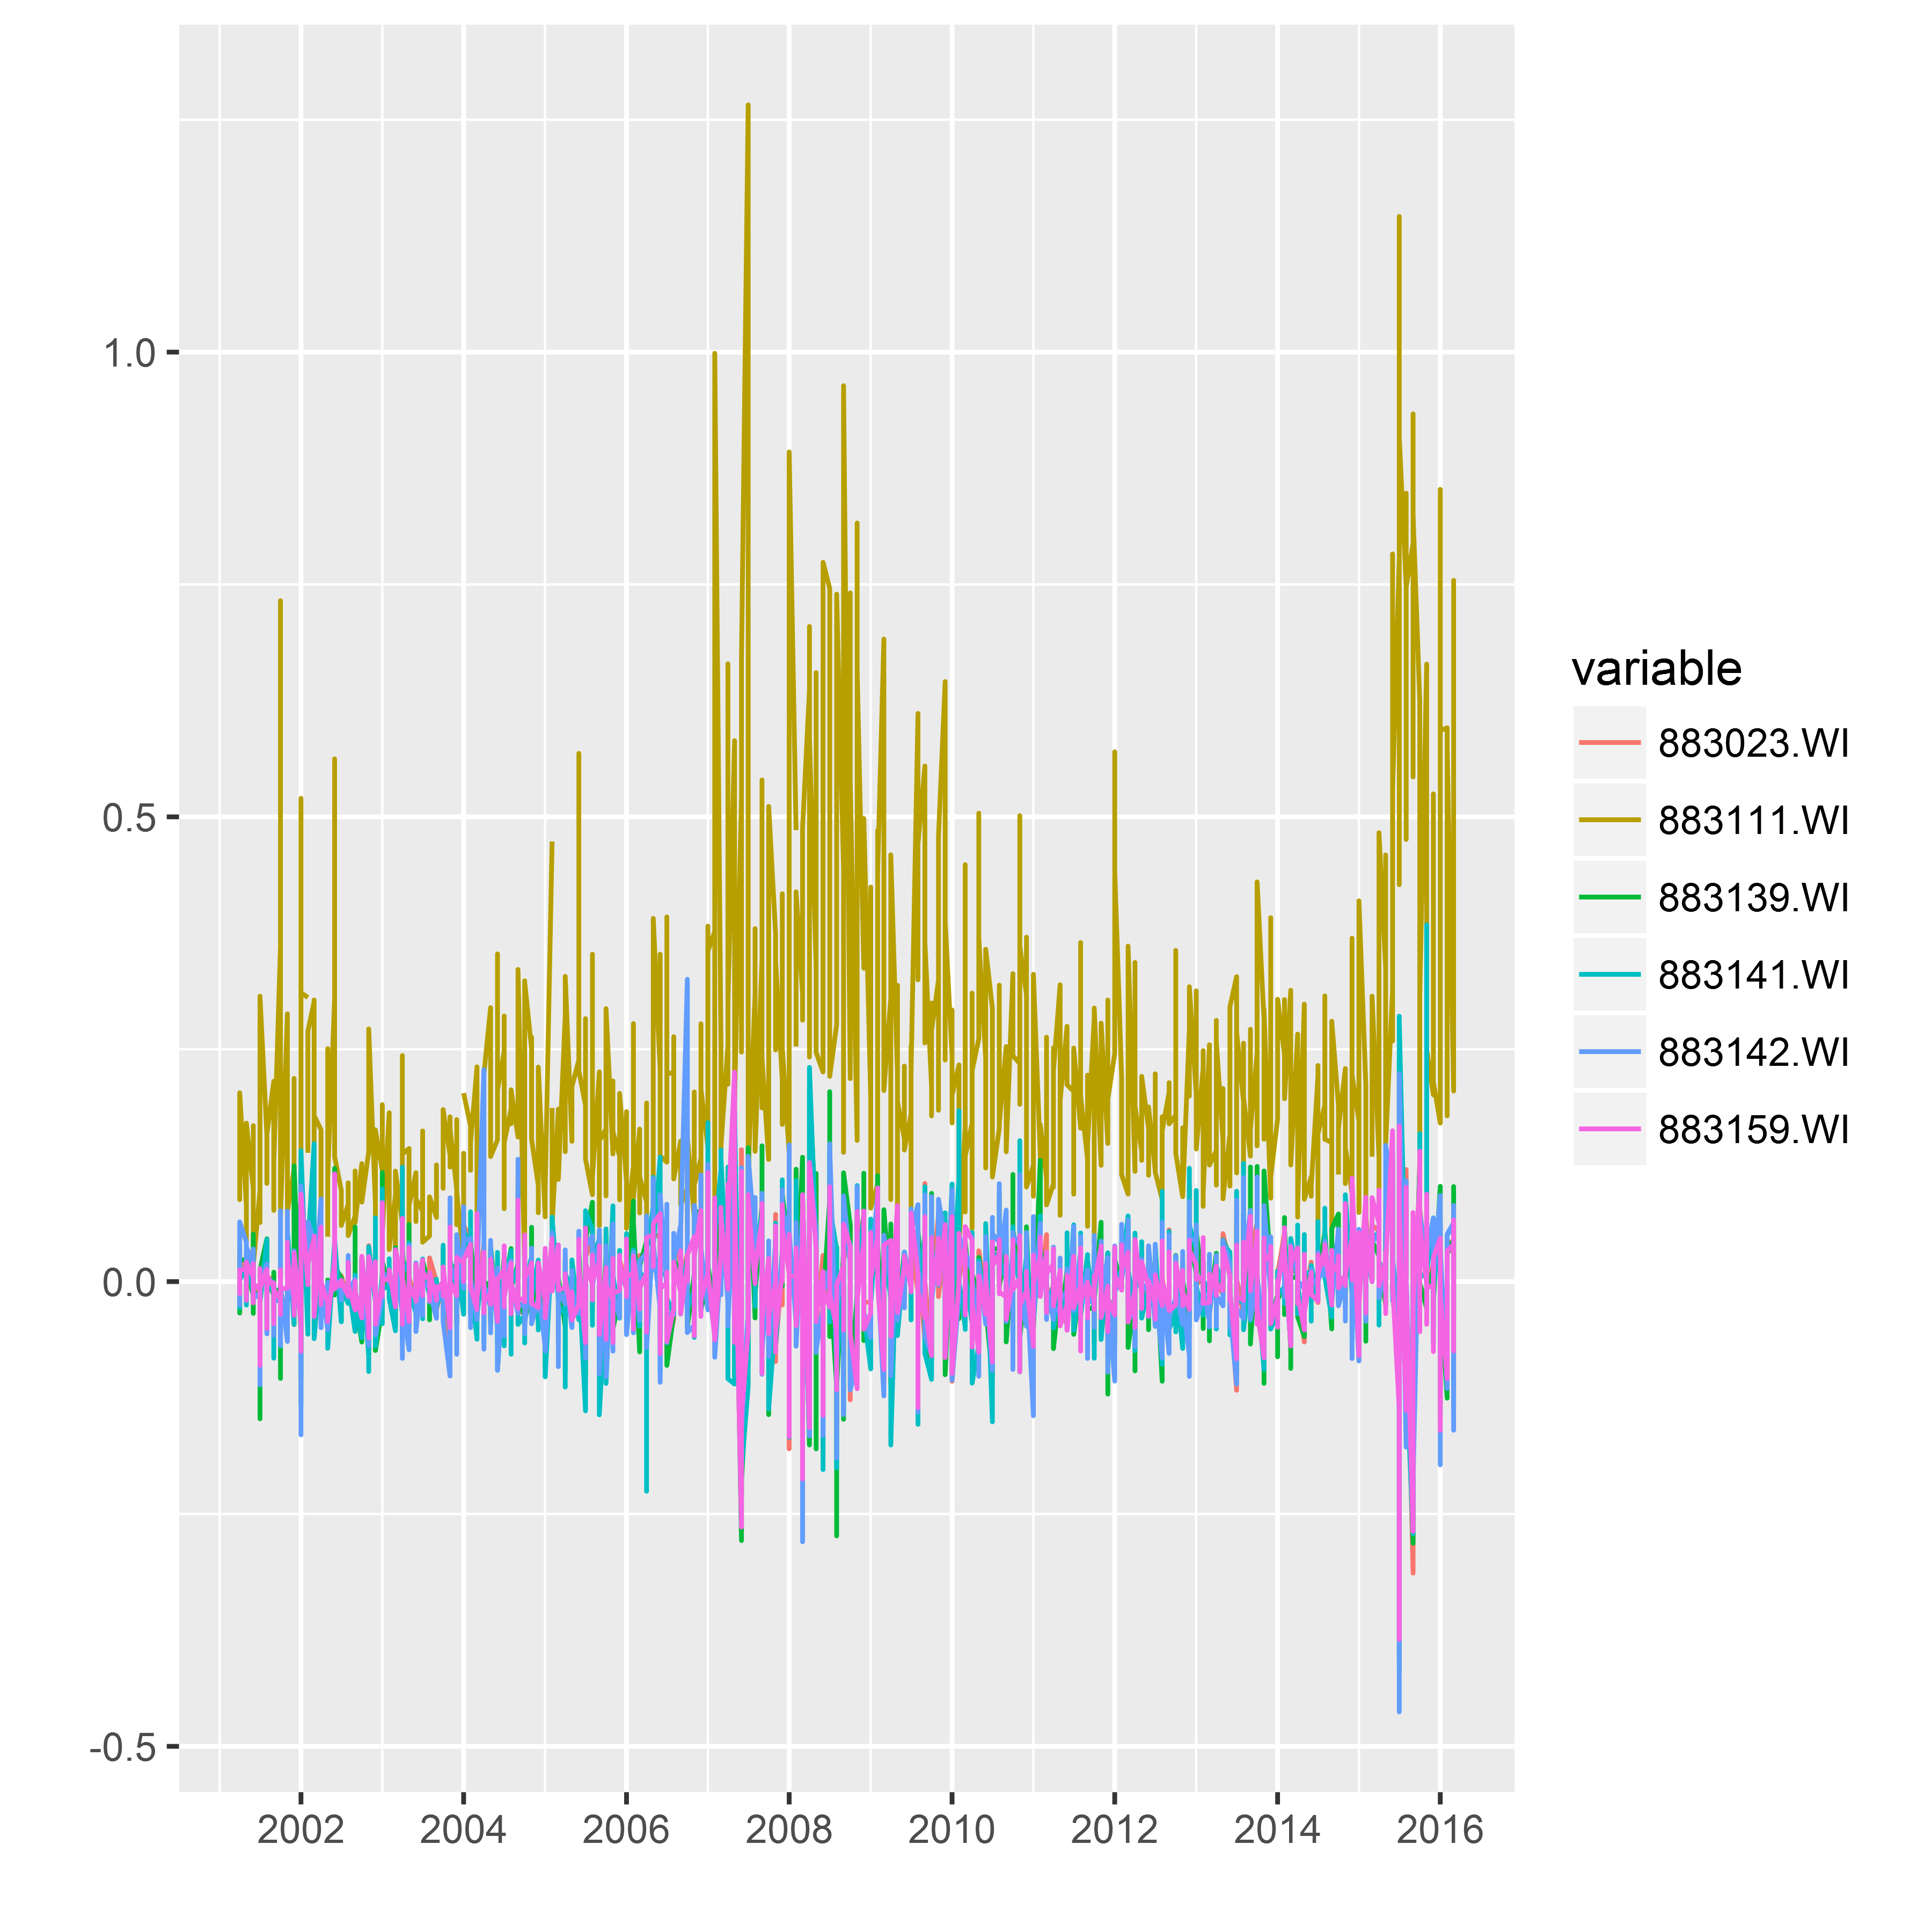
\includegraphics[scale=0.8]{image/883111-topk-upper-plus-one-weeklyvol-combined.png}
\caption{食品加工行业指数与关联最密切的五个上游行业指数的周波动率(年化)序列-指数同期叠加}
\caption*{\footnotesize 该图记录了食品加工行业指数与关联最密切的五个上游行业指数的历史周波动率的折线图,$X$轴是时间,从2001年4月第一周开始,到2016年3月最后一周。$Y$轴是年化了的历史周波动率。每种颜色代表一个行业指数的历史周波动率序列。}
\label{fig:883111-topk-upper-plus-one-weeklyvol-combined}
\end{figure}
\begin{figure}[htbp]
\centering
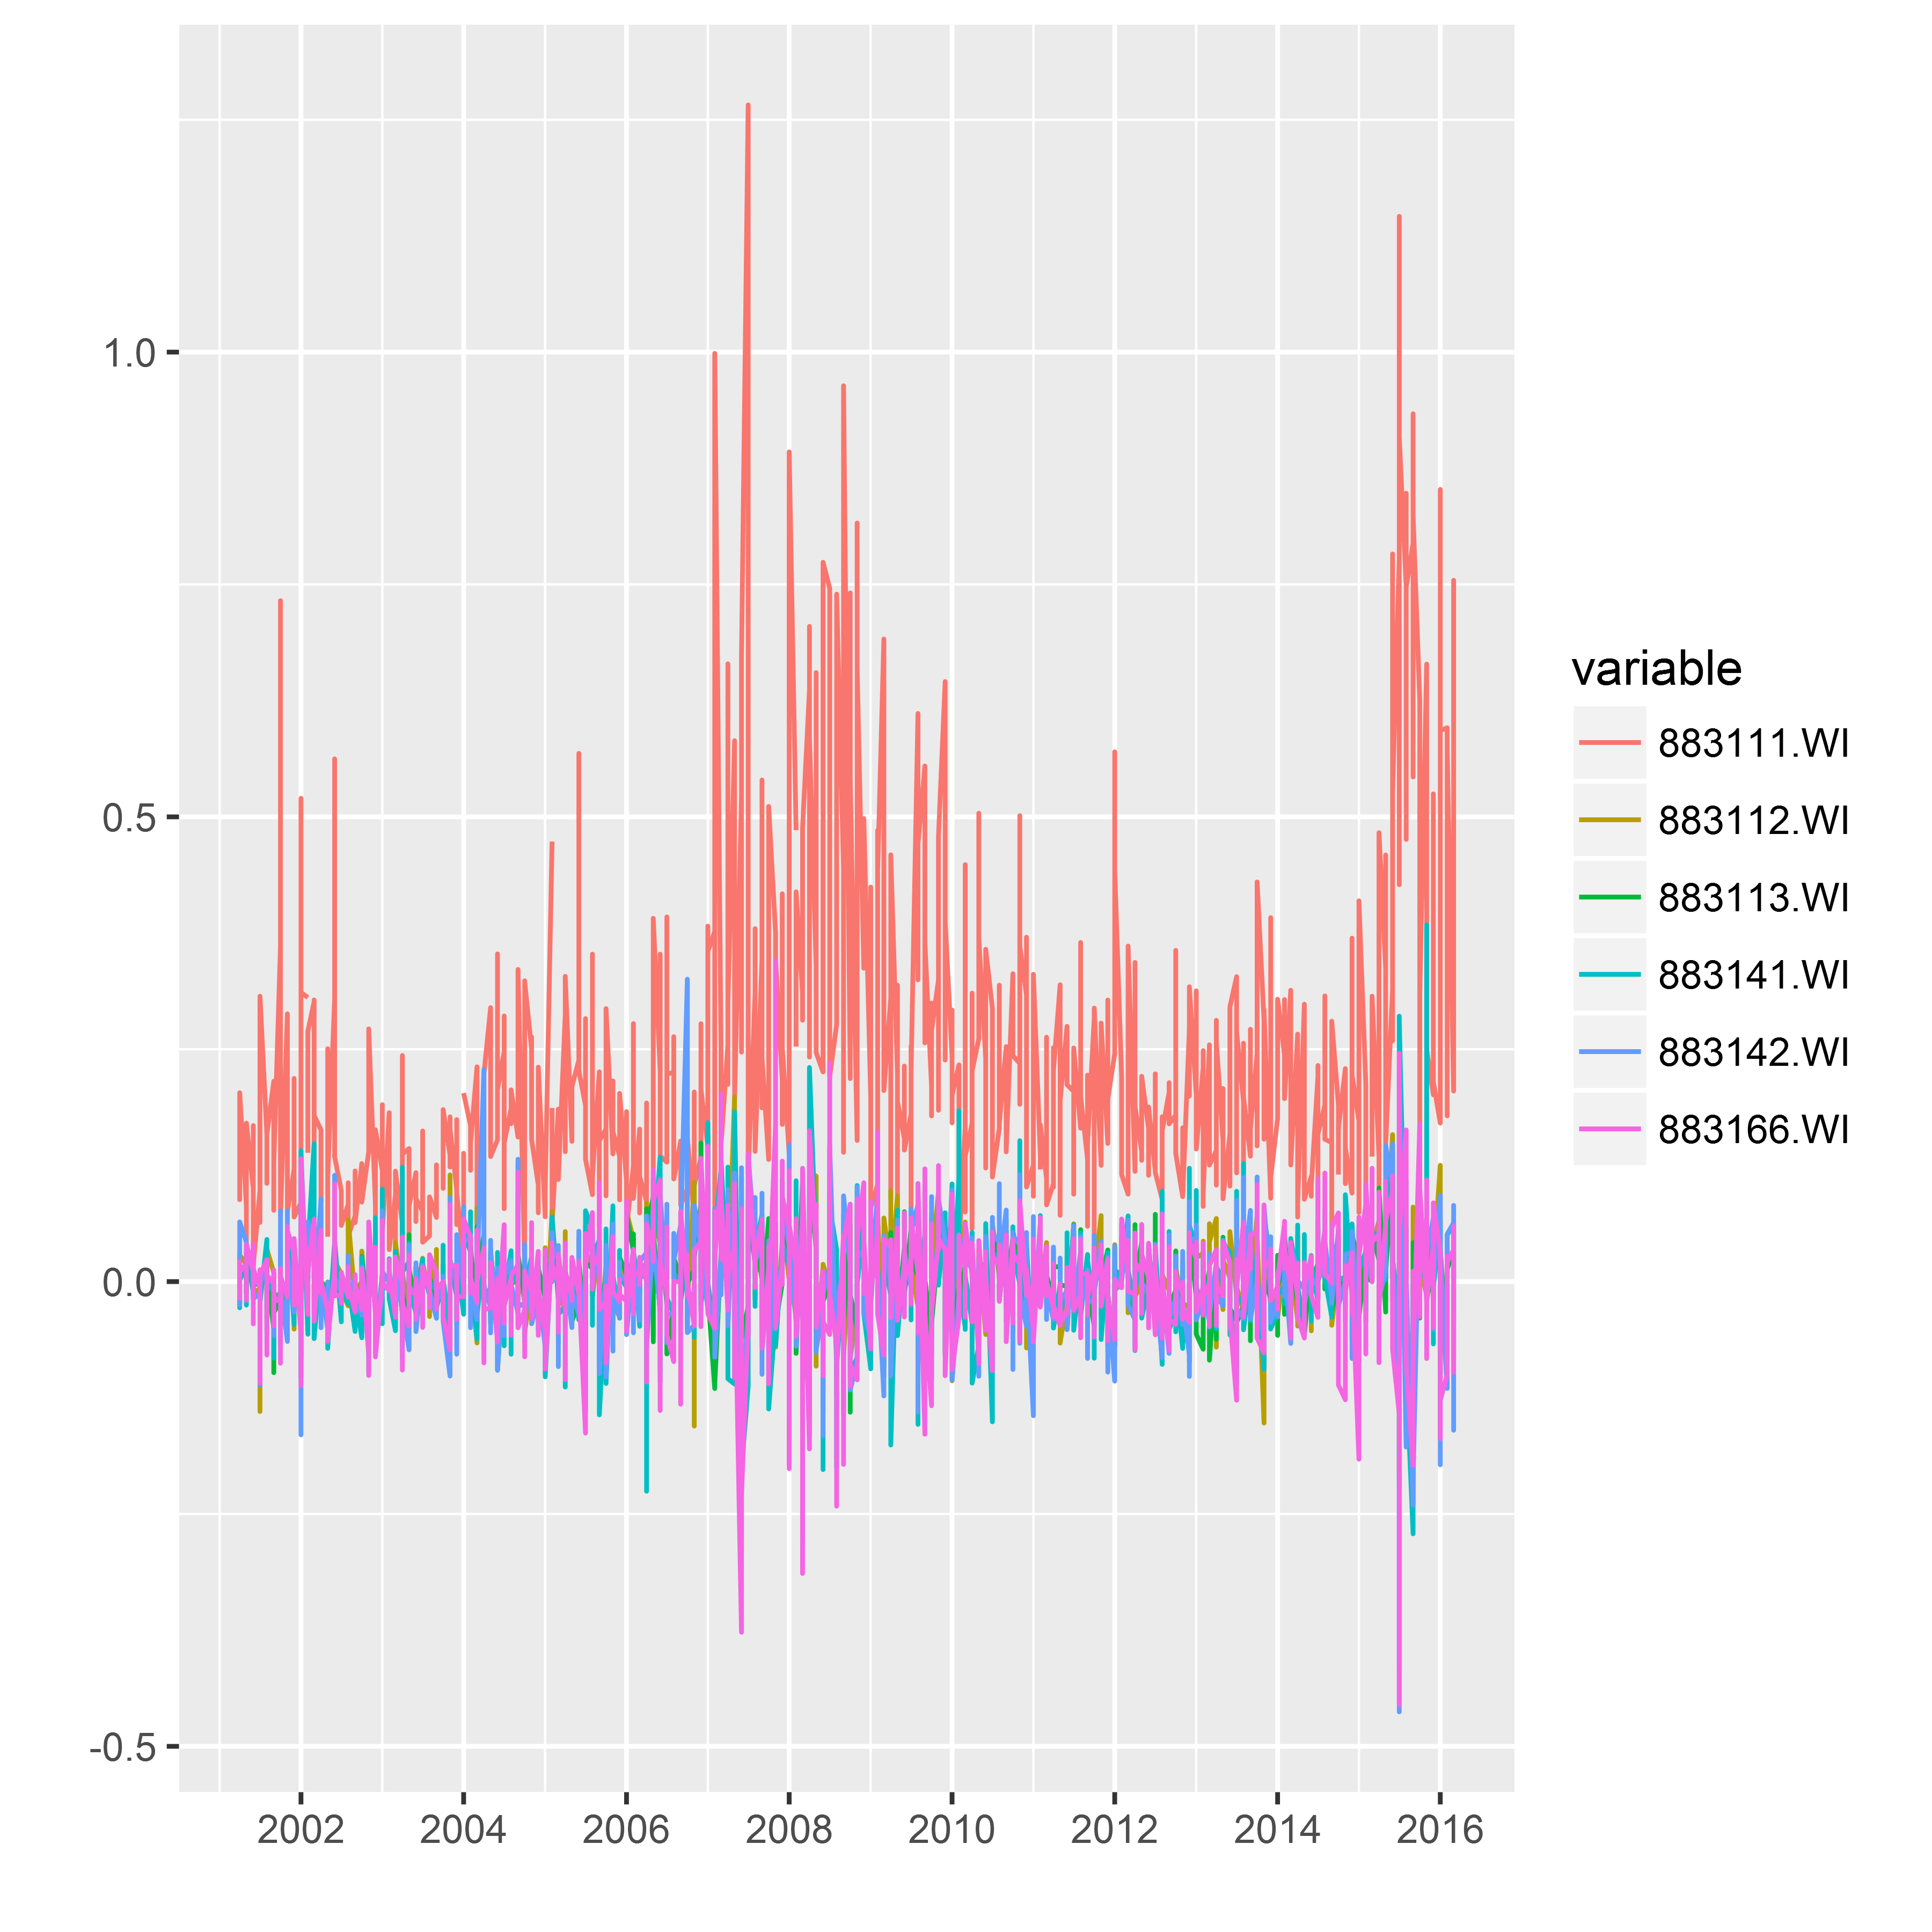
\includegraphics[scale=0.8]{image/883111-topk-lower-plus-one-weeklyvol-combined.png}
\caption{食品加工行业指数与关联最密切的五个下游行业指数的周波动率(年化)序列-指数同期叠加}
\caption*{\footnotesize 该图记录了食品加工行业指数与关联最密切的五个下游行业指数的历史周波动率的折线图,$X$轴是时间,从2001年4月第一周开始,到2016年3月最后一周。$Y$轴是年化了的历史周波动率。每种颜色代表一个行业指数的历史周波动率序列。}
\label{fig:883111-topk-lower-plus-one-weeklyvol-combined}
\end{figure}

% Table created by stargazer v.5.2 by Marek Hlavac, Harvard University. E-mail: hlavac at fas.harvard.edu
% Date and time: 周五, 五月 13, 2016 - 22:08:16
\chapter{全行业指数的周收益率及周波动率回归结果}

为了进一步探讨溢出效应是否存在于所有行业中,遍历所有行业,将每个行业的上游行业和下游行业的收益率和波动率序列分别获取。再用式\ref{least-square-yield}和式\ref{least-square-volatility}的方法,做最小二乘回归。得到的结果如下

\begin{table}[!htbp] \centering 
\caption{全行业周波动率与上下游行业周收益率回归的系数估计} 
  \caption*{\footnotesize 该表格记录所有行业及相关上下游行业的周收益率序列构成的面板数据的最小二乘回归系数估计。第一行和第二行分别是延滞一阶的重组的上游行业指数及重组的下游行业指数的周收益率估计值,第三行是全行业的周收益率序列的截距的估计值,重组时各取5个上游行业和5个下游行业,权重计算见式\ref{yield-weighted}。括号中是各系数估计值的标准差估计值。其中$p$是估计系数为零的零假设为真的概率。显著性记号分别为:{$^{*}$p$<$0.1; $^{**}$p$<$0.05; $^{***}$p$<$0.01}} 
  \renewcommand{\arraystretch}{0.5}
\begin{tabular}{@{\extracolsep{5pt}}lc} 
\\[-1.8ex]\hline 
\hline \\[-1.8ex] 
 & \multicolumn{1}{c}{\textit{因变量:}} \\ 
\cline{2-2} 
\\[-1.8ex] & 行业指数 \\ 
\hline \\[-1.8ex] 
 上游行业指数 & 0.051$^{***}$ \\ 
  & (0.008) \\ 
  & \\ 
 下游行业指数 & 0.055$^{***}$ \\ 
  & (0.007) \\ 
  & \\ 
 截距 & 0.001$^{***}$ \\ 
  & (0.0002) \\ 
  & \\ 
\hline \\[-1.8ex] 
Observations & 56,867 \\ 
R$^{2}$ & 0.008 \\ 
Adjusted R$^{2}$ & 0.008 \\ 
Residual Std. Error & 0.053 (df = 56864) \\ 
F Statistic & 217.066$^{***}$ (df = 2; 56864) \\ 
\hline 
\hline \\[-1.8ex] 
\textit{Note:}  & \multicolumn{1}{r}{$^{*}$p$<$0.1; $^{**}$p$<$0.05; $^{***}$p$<$0.01} \\ 
\end{tabular} 
\end{table} 

\begin{table}[!htbp] \centering 
\caption{全行业周波动率与上下游行业周波动率回归的系数估计} 
  \caption*{\footnotesize 该表格记录所有行业及相关上下游行业的周波动率序列构成的面板数据的最小二乘回归系数估计。第一行和第二行分别是延滞一阶的重组的上游行业指数及重组的下游行业指数的周波动率估计值,第三行是全行业的周波动率序列的截距的估计值,重组时各取5个上游行业和5个下游行业,权重计算见式\ref{volatility-weighted}。括号中是各系数估计值的标准差估计值。其中$p$是估计系数为零的零假设为真的概率。显著性记号分别为:{$^{*}$p$<$0.1; $^{**}$p$<$0.05; $^{***}$p$<$0.01}} 
  \renewcommand{\arraystretch}{0.5}
\begin{tabular}{@{\extracolsep{5pt}}lc} 
\\[-1.8ex]\hline 
\hline \\[-1.8ex] 
 & \multicolumn{1}{c}{\textit{因变量:}} \\ 
\cline{2-2} 
\\[-1.8ex] & 行业指数\\ 
\hline \\[-1.8ex] 
 上游行业指数 & 0.278$^{***}$ \\ 
  & (0.010) \\ 
  & \\ 
 下游行业指数 & 0.165$^{***}$ \\ 
  & (0.010) \\ 
  & \\ 
 截距 & 0.184$^{***}$ \\ 
  & (0.002) \\ 
  & \\ 
\hline \\[-1.8ex] 
Observations & 53,436 \\ 
R$^{2}$ & 0.112 \\ 
Adjusted R$^{2}$ & 0.112 \\ 
Residual Std. Error & 0.214 (df = 53433) \\ 
F Statistic & 3,385.349$^{***}$ (df = 2; 53433) \\ 
\hline 
\hline \\[-1.8ex] 
\textit{Note:}  & \multicolumn{1}{r}{$^{*}$p$<$0.1; $^{**}$p$<$0.05; $^{***}$p$<$0.01} \\ 
\end{tabular} 
\end{table} 


% Table created by stargazer v.5.2 by Marek Hlavac, Harvard University. E-mail: hlavac at fas.harvard.edu
% Date and time: 周六, 五月 14, 2016 - 10:22:38
\begin{table}[!htbp] \centering 
\caption{全行业周波动率与上下游行业周收益率回归的系数估计} 
  \caption*{\footnotesize 该表格记录所有行业及相关上下游行业的周收益率序列构成的面板数据的最小二乘回归系数估计。第一行和第二行分别是延滞一阶的重组的上游行业指数及重组的下游行业指数的周收益率估计值,第三行是全行业的周波动率序列的截距的估计值,重组时各取10个上游行业和10个下游行业,权重计算见式\ref{yield-weighted}。括号中是各系数估计值的标准差估计值。其中$p$是估计系数为零的零假设为真的概率。显著性记号分别为:{$^{*}$p$<$0.1; $^{**}$p$<$0.05; $^{***}$p$<$0.01}} 
  \renewcommand{\arraystretch}{0.5}
\begin{tabular}{@{\extracolsep{5pt}}lc} 
\\[-1.8ex]\hline 
\hline \\[-1.8ex] 
 & \multicolumn{1}{c}{\textit{Dependent variable:}} \\ 
\cline{2-2} 
\\[-1.8ex] & weeklyyield.allout[1, ] \\ 
\hline \\[-1.8ex] 
 weeklyyield.allout[2, ] & 0.040$^{***}$ \\ 
  & (0.012) \\ 
  & \\ 
 weeklyyield.allout[3, ] & 0.074$^{***}$ \\ 
  & (0.011) \\ 
  & \\ 
 Constant & 0.001$^{***}$ \\ 
  & (0.0002) \\ 
  & \\ 
\hline \\[-1.8ex] 
Observations & 56,867 \\ 
R$^{2}$ & 0.008 \\ 
Adjusted R$^{2}$ & 0.008 \\ 
Residual Std. Error & 0.053 (df = 56864) \\ 
F Statistic & 234.624$^{***}$ (df = 2; 56864) \\ 
\hline 
\hline \\[-1.8ex] 
\textit{Note:}  & \multicolumn{1}{r}{$^{*}$p$<$0.1; $^{**}$p$<$0.05; $^{***}$p$<$0.01} \\ 
\end{tabular} 
\end{table} 



\begin{table}[!htbp] \centering 
\caption{全行业周波动率与上下游行业周波动率回归的系数估计} 
  \caption*{\footnotesize 该表格记录所有行业及相关上下游行业的周波动率序列构成的面板数据的最小二乘回归系数估计。第一行和第二行分别是延滞一阶的重组的上游行业指数及重组的下游行业指数的周波动率估计值,第三行是全行业的周波动率序列的截距的估计值,重组时各取10个上游行业和10个下游行业,权重计算见式\ref{volatility-weighted}。括号中是各系数估计值的标准差估计值。其中$p$是估计系数为零的零假设为真的概率。显著性记号分别为:{$^{*}$p$<$0.1; $^{**}$p$<$0.05; $^{***}$p$<$0.01}} 
  \renewcommand{\arraystretch}{0.5}
\begin{tabular}{@{\extracolsep{5pt}}lc} 
\\[-1.8ex]\hline 
\hline \\[-1.8ex] 
 & \multicolumn{1}{c}{\textit{Dependent variable:}} \\ 
\cline{2-2} 
\\[-1.8ex] & weeklyyield.allout[4, ] \\ 
\hline \\[-1.8ex] 
 weeklyyield.allout[5, ] & 0.301$^{***}$ \\ 
  & (0.011) \\ 
  & \\ 
 weeklyyield.allout[6, ] & 0.151$^{***}$ \\ 
  & (0.011) \\ 
  & \\ 
 Constant & 0.184$^{***}$ \\ 
  & (0.002) \\ 
  & \\ 
\hline \\[-1.8ex] 
Observations & 53,436 \\ 
R$^{2}$ & 0.115 \\ 
Adjusted R$^{2}$ & 0.115 \\ 
Residual Std. Error & 0.213 (df = 53433) \\ 
F Statistic & 3,474.981$^{***}$ (df = 2; 53433) \\ 
\hline 
\hline \\[-1.8ex] 
\textit{Note:}  & \multicolumn{1}{r}{$^{*}$p$<$0.1; $^{**}$p$<$0.05; $^{***}$p$<$0.01} \\ 
\end{tabular} 
\end{table} 


\chapter{偏度和波动率的回归结果}

以周数据为频率,分别对负系数偏度(NCSKEW)和下跌到上升波动率(DUVOL)进行回归,回归的关系分别满足式\ref{NCSKEW_Regression}及式\ref{DUVOL_Regression}。而NCSKEW和DUVOL的计算公式分别为\ref{NCSKEW_Calculation}及式\ref{DUVOL_Calculation}。计算的采样周期分别为双周和月。
\begin{equation}
\label{NCSKEW_Regression}
{NCSKEW_{i,t}} = {\beta _{i,upper,t - 1}}{NCSKEW_{i,upper,t - 1}} + {\beta _{i,lower,t - 1}}{NCSKEW_{i,lower,t - 1}} + {\varepsilon _{i,t}}
\end{equation}

\begin{equation}
\label{DUVOL_Regression}
{DUVOL_{i,t}} = {\beta _{i,upper,t - 1}}{DUVOL_{i,upper,t - 1}} + {\beta _{i,lower,t - 1}}{DUVOL_{i,lower,t - 1}} + {\varepsilon _{i,t}}
\end{equation}

\begin{equation}
\label{NCSKEW_Calculation}
NCSKEW =  - \frac{{\sum {{{({R_{i,t}})}^3}} n{{(n - 1)}^{\frac{3}{2}}}}}{{\sum {{{({{({R_{i,t}})}^2})}^{\frac{3}{2}}}} (n - 1)(n - 2)}}
\end{equation}

式\ref{NCSKEW_Calculation}中,$R_{i,t}$是行业指数$i$在时间区域$t$内的每日对数收益率,分别求出该时间区域内的三阶样本矩及二阶样本矩,得到偏度和方差,$n$是对应的这一个时间范围中交易的天数。类似地,我们可以得到负系数偏度的加权上游负偏度系数和加权下游副偏度系数,计算公式为式\ref{NCSKEW-upper-recombined}及式\ref{NCSKEW-lower-recombined}。

\begin{equation}
\label{NCSKEW-upper-recombined} 
{NCSKEW’_{upper}} = \sum\limits_{i = 1}^k {{NCSKEW_{upper,i}}{w_i}} 
\end{equation}

${NCSKEW’_{upper}}$是组合后的上游行业的负系数偏度序列,${NCSKEW_{upper,i}}$是上游行业中,联系最大的第i个行业对应的行业指数的负系数偏度序列,$k$是除去自身以外,囊括的行业指数的数量,${w_i}$则为第$i$个指数的中间流量权重。

\begin{equation}
\label{NCSKEW-lower-recombined} 
{NCSKEW’_{lower}} = \sum\limits_{i = 1}^k {{NCSKEW_{lower,i}}{w_i}} 
\end{equation}

${NCSKEW’_{lower}}$是组合后的下游行业的负系数偏度序列,${NCSKEW_{lower,i}}$是下游行业中,联系最大的第i个行业对应的行业指数的负系数偏度序列,$k$是除去自身以外,囊括的行业指数的数量,${w_i}$则为第$i$个指数的中间流量权重。

\begin{equation}
\label{DUVOL_Calculation}
DUVOL = \log (\frac{{({n_{positive,t}} - 1)\sum\limits_{negative} {R_{i,negative,t}^2} }}{{({n_{negative,t}} - 1)\sum\limits_{positive} {{R_{i,positive,t}}} }})
\end{equation}

式\ref{DUVOL_Regression}中,$R_{i,positive,t}$是行业指数$i$在时间区域$t$内正的对数收益率,$R_{i,negative,t}$是时间区域$t$内负的对数收益率,求出该时间区域内正的对数收益率的方差及负的对数收益率的方差,$n_{i,positive,t}$是行业指数$i$在时间区域$t$中,收益率为正的交易天数,$n_{i,negative,t}$是行业指数$i$在时间区域$t$中,收益率为负的交易天数。

由于式\ref{DUVOL_Calculation}及式\ref{NCSKEW_Calculation}中,都带有形如$(n-k)$的项,其中$k$是一个正整数,所以,如果以周作为计算指标的区间,尤其是计算DUVOL时,会由于区间内正的或负的交易天数小于或等于k,导致结果可能出现无穷大,针对这种可能,我们对结果做了一个判定,出现这些值的情况,都统一置为0。为了确保有足够的样本点,时间区间不能太宽,即每个$t$中包含的交易天数不能太多。因此,找一个平衡点,让时间区间定为双周和一个月,分别作回归,得到的结果为:


% Table created by stargazer v.5.2 by Marek Hlavac, Harvard University. E-mail: hlavac at fas.harvard.edu
% Date and time: 周二, 五月 31, 2016 - 20:25:55
\begin{table}[!htbp] \centering 
\caption{全行业负系数偏度与上下游行业负系数偏度回归的系数估计-以双周为间隔} 
  \caption*{\footnotesize 该表格记录所有行业及相关上下游行业的负系数偏度序列构成的面板数据的最小二乘回归系数估计。第一行和第二行分别是延滞一阶的重组的上游行业指数及重组的下游行业指数的负系数偏度估计值,第三行是全行业的负系数偏度序列的截距的估计值,重组时各取10个上游行业和5个下游行业,权重计算见式\ref{NCSKEW_Calculation}。括号中是各系数估计值的标准差估计值。其中$p$是估计系数为零的零假设为真的概率。显著性记号分别为:{$^{*}$p$<$0.1; $^{**}$p$<$0.05; $^{***}$p$<$0.01}} 
  \renewcommand{\arraystretch}{0.5}
\begin{tabular}{@{\extracolsep{5pt}}lc} 
\\[-1.8ex]\hline 
\hline \\[-1.8ex] 
 & \multicolumn{1}{c}{\textit{Dependent variable:}} \\ 
\cline{2-2} 
\\[-1.8ex] & 行业在t的NCSKEW \\ 
\hline \\[-1.8ex] 
 NCSKEW\_{上游,t-1} & $-$0.009 \\ 
  & (0.011) \\ 
  & \\ 
 NCSKEW\_{下游,t-1} & 0.006 \\ 
  & (0.011) \\ 
  & \\ 
 Constant & 0.074$^{***}$ \\ 
  & (0.025) \\ 
  & \\ 
\hline \\[-1.8ex] 
Observations & 26,647 \\ 
R$^{2}$ & 0.00003 \\ 
Adjusted R$^{2}$ & $-$0.00005 \\ 
Residual Std. Error & 4.044 (df = 26644) \\ 
F Statistic & 0.389 (df = 2; 26644) \\ 
\hline 
\hline \\[-1.8ex] 
\textit{Note:}  & \multicolumn{1}{r}{$^{*}$p$<$0.1; $^{**}$p$<$0.05; $^{***}$p$<$0.01} \\ 
\end{tabular} 
\end{table} 


% Table created by stargazer v.5.2 by Marek Hlavac, Harvard University. E-mail: hlavac at fas.harvard.edu
% Date and time: 周二, 五月 31, 2016 - 20:25:59
\begin{table}[!htbp] \centering 
\caption{全行业负系数偏度与上下游行业负系数偏度回归的系数估计-以一个月为间隔} 
  \caption*{\footnotesize 该表格记录所有行业及相关上下游行业的负系数偏度序列构成的面板数据的最小二乘回归系数估计。第一行和第二行分别是延滞一阶的重组的上游行业指数及重组的下游行业指数的负系数偏度估计值,第三行是全行业的负系数偏度的截距的估计值,重组时各取10个上游行业和5个下游行业,权重计算见式\ref{NCSKEW_Calculation}。括号中是各系数估计值的标准差估计值。其中$p$是估计系数为零的零假设为真的概率。显著性记号分别为:{$^{*}$p$<$0.1; $^{**}$p$<$0.05; $^{***}$p$<$0.01}} 
  \renewcommand{\arraystretch}{0.5}
\begin{tabular}{@{\extracolsep{5pt}}lc} 
\\[-1.8ex]\hline 
\hline \\[-1.8ex] 
 & \multicolumn{1}{c}{\textit{Dependent variable:}} \\ 
\cline{2-2} 
\\[-1.8ex] & 行业在t的NCSKEW \\ 
\hline \\[-1.8ex] 
 NCSKEW\_{上游,t-1} & $-$0.076$^{***}$ \\ 
  & (0.015) \\ 
  & \\ 
 NCSKEW\_{下游,t-1} & 0.029$^{*}$ \\ 
  & (0.015) \\ 
  & \\ 
 Constant & 0.505$^{***}$ \\ 
  & (0.042) \\ 
  & \\ 
\hline \\[-1.8ex] 
Observations & 12,287 \\ 
R$^{2}$ & 0.003 \\ 
Adjusted R$^{2}$ & 0.003 \\ 
Residual Std. Error & 4.540 (df = 12284) \\ 
F Statistic & 17.199$^{***}$ (df = 2; 12284) \\ 
\hline 
\hline \\[-1.8ex] 
\textit{Note:}  & \multicolumn{1}{r}{$^{*}$p$<$0.1; $^{**}$p$<$0.05; $^{***}$p$<$0.01} \\ 
\end{tabular} 
\end{table} 

% Table created by stargazer v.5.2 by Marek Hlavac, Harvard University. E-mail: hlavac at fas.harvard.edu
% Date and time: 周三, 六月 01, 2016 - 12:15:44
\begin{table}[!htbp] \centering 
\caption{全行业DUVOL与上下游行业DUVOL的系数估计-以双周为间隔} 
  \caption*{\footnotesize 该表格记录所有行业及相关上下游行业的DUVOL序列构成的面板数据的最小二乘回归系数估计。第一行和第二行分别是延滞一阶的重组的上游行业指数及重组的下游行业指数的DUVOL估计值,第三行是全行业的DUVOL的截距的估计值,重组时各取5个上游行业和5个下游行业,权重计算见式\ref{DUVOL_Calculation}。括号中是各系数估计值的标准差估计值。其中$p$是估计系数为零的零假设为真的概率。显著性记号分别为:{$^{*}$p$<$0.1; $^{**}$p$<$0.05; $^{***}$p$<$0.01}} 
  \renewcommand{\arraystretch}{0.5}
\begin{tabular}{@{\extracolsep{5pt}}lc} 
\\[-1.8ex]\hline 
\hline \\[-1.8ex] 
 & \multicolumn{1}{c}{\textit{Dependent variable:}} \\ 
\cline{2-2} 
\\[-1.8ex] & DUVOL \\ 
\hline \\[-1.8ex] 
 DUVOL\_u & 0.012 \\ 
  & (0.008) \\ 
  & \\ 
 DUVOL\_l & $-$0.017$^{**}$ \\ 
  & (0.008) \\ 
  & \\ 
 Constant & 0.119$^{***}$ \\ 
  & (0.010) \\ 
  & \\ 
\hline \\[-1.8ex] 
Observations & 22,360 \\ 
R$^{2}$ & 0.0002 \\ 
Adjusted R$^{2}$ & 0.0001 \\ 
Residual Std. Error & 1.449 (df = 22357) \\ 
F Statistic & 2.432$^{*}$ (df = 2; 22357) \\ 
\hline 
\hline \\[-1.8ex] 
\textit{Note:}  & \multicolumn{1}{r}{$^{*}$p$<$0.1; $^{**}$p$<$0.05; $^{***}$p$<$0.01} \\ 
\end{tabular} 
\end{table} 


% Table created by stargazer v.5.2 by Marek Hlavac, Harvard University. E-mail: hlavac at fas.harvard.edu
% Date and time: 周三, 六月 01, 2016 - 12:15:38
\begin{table}[!htbp] \centering 
\caption{全行业DUVOL与上下游行业DUVOL的系数估计-以月为间隔} 
  \caption*{\footnotesize 该表格记录所有行业及相关上下游行业的DUVOL序列构成的面板数据的最小二乘回归系数估计。第一行和第二行分别是延滞一阶的重组的上游行业指数及重组的下游行业指数的DUVOL估计值,第三行是全行业的DUVOL的截距的估计值,重组时各取5个上游行业和5个下游行业,权重计算见式\ref{DUVOL_Calculation}。括号中是各系数估计值的标准差估计值。其中$p$是估计系数为零的零假设为真的概率。显著性记号分别为:{$^{*}$p$<$0.1; $^{**}$p$<$0.05; $^{***}$p$<$0.01}} 
  \renewcommand{\arraystretch}{0.5}
\begin{tabular}{@{\extracolsep{5pt}}lc} 
\\[-1.8ex]\hline 
\hline \\[-1.8ex] 
 & \multicolumn{1}{c}{\textit{Dependent variable:}} \\ 
\cline{2-2} 
\\[-1.8ex] & DUVOL \\ 
\hline \\[-1.8ex] 
 DUVOL\_u & 0.041$^{***}$ \\ 
  & (0.012) \\ 
  & \\ 
 DUVOL\_l & 0.053$^{***}$ \\ 
  & (0.011) \\ 
  & \\ 
 Constant & 0.175$^{***}$ \\ 
  & (0.010) \\ 
  & \\ 
\hline \\[-1.8ex] 
Observations & 12,269 \\ 
R$^{2}$ & 0.006 \\ 
Adjusted R$^{2}$ & 0.006 \\ 
Residual Std. Error & 1.041 (df = 12266) \\ 
F Statistic & 38.155$^{***}$ (df = 2; 12266) \\ 
\hline 
\hline \\[-1.8ex] 
\textit{Note:}  & \multicolumn{1}{r}{$^{*}$p$<$0.1; $^{**}$p$<$0.05; $^{***}$p$<$0.01} \\ 
\end{tabular} 
\end{table} 


\chapter{崩盘指标的计算}
崩盘指标是一个渐进的条件概率。崩盘值的定义为式\ref{Crash_Calculation}。
\begin{equation}
\label{Crash_Calculation}
Crash = \mathop {\lim }\limits_{q \to 0} \frac{{P(F({r_{sector}}) < q,F({r_{market}}) < q)}}{{P(F({r_{market}}) < q)}}
\end{equation}

其中,$q$是百分位数,取值为0到1.而$F({r_{sector}})$是行业的收益率在$T-12+1$个月到$T$个月期间的对数收益率的分布函数;$F({r_{market}})$是大盘的收益率在$T-12+1$个月到$T$个月期间的对数收益率的分布函数,大盘对应的指数是万得资讯终端中的万得A股指数。

例如,取分位数为0.05的时候,Crash指标对应的是当大盘收益率跌破往年收益率的后5\%百分数时,行业指数的收益率也跌破分位数5\%的概率。为了探究行业间崩盘值的关联,计算加权上游崩盘值和加权下游崩盘值,计算公式为式\ref{Crash-upper-recombined}及式\ref{Crash-lower-recombined}。

\begin{equation}
\label{Crash-upper-recombined} 
{Crash’_{upper}} = \sum\limits_{i = 1}^k {{w_i}{Crash_{upper,i}}} 
\end{equation}

${Crash’_{upper}}$是组合后的上游行业的崩盘值序列,${Crash_{upper,i}}$是上游行业中,联系最大的第i个行业对应的行业指数的崩盘值序列,$k$是除去自身以外,囊括的行业指数的数量,${w_i}$则为第$i$个指数的中间流量权重。

\begin{equation}
\label{Crash-lower-recombined} 
{NCSKEW’_{lower}} = \sum\limits_{i = 1}^k {{w_i}{NCSKEW_{lower,i}}} 
\end{equation}

${Crash’_{lower}}$是组合后的下游行业的崩盘之序列,${Crash_{lower,i}}$是下游行业中,联系最大的第i个行业对应的行业指数的崩盘值序列,$k$是除去自身以外,囊括的行业指数的数量,${w_i}$则为第$i$个指数的中间流量权重。

以年数据为频率,对行业自身的Crash及上下游行业的Crash进行回归,回归的关系满足式\ref{Crash_Regression}。
\begin{equation}
\label{Crash_Regression}
{Crash_{i,t}} = {\beta _{i,upper,t - 1}}{Crash_{i,upper,t - 1}} + {\beta _{i,lower,t - 1}}{Crash_{i,lower,t - 1}} + {\varepsilon _{i,t}}
\end{equation}

针对不同的分位数,不同的时间间隔分别做最小二乘回归,最小二乘回归的结果见\ref{Crash-Regression-Result-top5-biweekly-5percent},\ref{Crash-Regression-Result-top5-biweekly-10percent},\ref{Crash-Regression-Result-top5-monthly-5percent}及\ref{Crash-Regression-Result-top5-monthly-10percent}。

\begin{table}[!htbp] \centering 
\caption{全行业崩盘指标与上下游行业崩盘指标系数估计-以双周为间隔-以尾部5\%为临界点} 
  \caption*{\footnotesize 该表格记录所有行业及相关上下游行业的崩盘序列构成的面板数据的最小二乘回归系数估计。第一行和第二行分别是延滞一阶的重组的上游行业指数及重组的下游行业指数的崩盘指标估计值,第三行是全行业的崩盘指标的截距的估计值,重组时各取5个上游行业和5个下游行业,权重计算见式\ref{Crash-upper-recombined}及式\ref{Crash-lower-recombined}。括号中是各系数估计值的标准差估计值。其中$p$是估计系数为零的零假设为真的概率。显著性记号分别为:{$^{*}$p$<$0.1; $^{**}$p$<$0.05; $^{***}$p$<$0.01}} 
  \label{Crash-Regression-Result-top5-biweekly-5percent}
  \renewcommand{\arraystretch}{0.5}
\begin{tabular}{@{\extracolsep{5pt}}lc} 
\\[-1.8ex]\hline 
\hline \\[-1.8ex] 
 & \multicolumn{1}{c}{\textit{解释变量:}} \\ 
\cline{2-2} 
\\[-1.8ex] & 全行业 \\ 
\hline \\[-1.8ex] 
 下游行业延滞一阶 & 0.176$^{***}$ \\ 
  & (0.009) \\ 
  & \\ 
 上游行业延滞一阶 & 0.231$^{***}$ \\ 
  & (0.011) \\ 
  & \\ 
 截距 & 0.259$^{***}$ \\ 
  & (0.009) \\ 
  & \\ 
\hline \\[-1.8ex] 
Observations & 26,499 \\ 
R$^{2}$ & 0.042 \\ 
Adjusted R$^{2}$ & 0.042 \\ 
Residual Std. Error & 0.216 (df = 26496) \\ 
F Statistic & 577.337$^{***}$ (df = 2; 26496) \\ 
\hline 
\hline \\[-1.8ex] 
\textit{Note:}  & \multicolumn{1}{r}{$^{*}$p$<$0.1; $^{**}$p$<$0.05; $^{***}$p$<$0.01} \\ 
\end{tabular} 
\end{table} 

\begin{table}[!htbp] \centering 
\caption{全行业崩盘指标与上下游行业崩盘指标系数估计-以双周为间隔-以尾部10\%为临界点} 
  \caption*{\footnotesize 该表格记录所有行业及相关上下游行业的崩盘序列构成的面板数据的最小二乘回归系数估计。第一行和第二行分别是延滞一阶的重组的上游行业指数及重组的下游行业指数的崩盘指标估计值,第三行是全行业的崩盘指标的截距的估计值,重组时各取5个上游行业和5个下游行业,权重计算见式\ref{Crash-upper-recombined}及式\ref{Crash-lower-recombined}。括号中是各系数估计值的标准差估计值。其中$p$是估计系数为零的零假设为真的概率。显著性记号分别为:{$^{*}$p$<$0.1; $^{**}$p$<$0.05; $^{***}$p$<$0.01}} 
  \label{Crash-Regression-Result-top5-biweekly-10percent}
  \renewcommand{\arraystretch}{0.5}
\begin{tabular}{@{\extracolsep{5pt}}lc} 
\\[-1.8ex]\hline 
\hline \\[-1.8ex] 
 & \multicolumn{1}{c}{\textit{解释变量:}} \\ 
\cline{2-2} 
\\[-1.8ex] & 全行业 \\ 
\hline \\[-1.8ex] 
 下游行业延滞一阶 & 0.178$^{***}$ \\ 
  & (0.011) \\ 
  & \\ 
 上游行业延滞一阶 & 0.123$^{***}$ \\ 
  & (0.013) \\ 
  & \\ 
 截距 & 0.379$^{***}$ \\ 
  & (0.011) \\ 
  & \\ 
\hline \\[-1.8ex] 
Observations & 26,499 \\ 
R$^{2}$ & 0.018 \\ 
Adjusted R$^{2}$ & 0.018 \\ 
Residual Std. Error & 0.200 (df = 26496) \\ 
F Statistic & 244.361$^{***}$ (df = 2; 26496) \\ 
\hline 
\hline \\[-1.8ex] 
\textit{Note:}  & \multicolumn{1}{r}{$^{*}$p$<$0.1; $^{**}$p$<$0.05; $^{***}$p$<$0.01} \\ 
\end{tabular} 
\end{table} 

% Table created by stargazer v.5.2 by Marek Hlavac, Harvard University. E-mail: hlavac at fas.harvard.edu
% Date and time: 周日, 六月 12, 2016 - 10:33:24
\begin{table}[!htbp] \centering 
\caption{全行业崩盘指标与上下游行业崩盘指标系数估计-以月为间隔-以尾部5\%为临界点} 
  \caption*{\footnotesize 该表格记录所有行业及相关上下游行业的崩盘序列构成的面板数据的最小二乘回归系数估计。第一行和第二行分别是延滞一阶的重组的上游行业指数及重组的下游行业指数的崩盘指标估计值,第三行是全行业的崩盘指标的截距的估计值,重组时各取5个上游行业和5个下游行业,权重计算见式\ref{Crash-upper-recombined}及式\ref{Crash-lower-recombined}。括号中是各系数估计值的标准差估计值。其中$p$是估计系数为零的零假设为真的概率。显著性记号分别为:{$^{*}$p$<$0.1; $^{**}$p$<$0.05; $^{***}$p$<$0.01}} 
  \label{Crash-Regression-Result-top5-monthly-5percent}
  \renewcommand{\arraystretch}{0.5}
\begin{tabular}{@{\extracolsep{5pt}}lc} 
\\[-1.8ex]\hline 
\hline \\[-1.8ex] 
 & \multicolumn{1}{c}{\textit{解释变量:}} \\ 
\cline{2-2} 
\\[-1.8ex] & 全行业 \\ 
\hline \\[-1.8ex] 
 下游行业延滞一阶 & 0.171$^{***}$ \\ 
  & (0.013) \\ 
  & \\ 
 上游行业延滞一阶 & 0.219$^{***}$ \\ 
  & (0.016) \\ 
  & \\ 
 截距 & 0.273$^{***}$ \\ 
  & (0.013) \\ 
  & \\ 
\hline \\[-1.8ex] 
Observations & 12,410 \\ 
R$^{2}$ & 0.038 \\ 
Adjusted R$^{2}$ & 0.038 \\ 
Residual Std. Error & 0.216 (df = 12407) \\ 
F Statistic & 247.363$^{***}$ (df = 2; 12407) \\ 
\hline 
\hline \\[-1.8ex] 
\textit{Note:}  & \multicolumn{1}{r}{$^{*}$p$<$0.1; $^{**}$p$<$0.05; $^{***}$p$<$0.01} \\ 
\end{tabular} 
\end{table} 


% Table created by stargazer v.5.2 by Marek Hlavac, Harvard University. E-mail: hlavac at fas.harvard.edu
% Date and time: 周日, 六月 12, 2016 - 10:33:24
\begin{table}[!htbp] \centering 
\caption{全行业崩盘指标与上下游行业崩盘指标系数估计-以月为间隔-以尾部10\%为临界点} 
  \caption*{\footnotesize 该表格记录所有行业及相关上下游行业的崩盘序列构成的面板数据的最小二乘回归系数估计。第一行和第二行分别是延滞一阶的重组的上游行业指数及重组的下游行业指数的崩盘指标估计值,第三行是全行业的崩盘指标的截距的估计值,重组时各取5个上游行业和5个下游行业,权重计算见式\ref{Crash-upper-recombined}及式\ref{Crash-lower-recombined}。括号中是各系数估计值的标准差估计值。其中$p$是估计系数为零的零假设为真的概率。显著性记号分别为:{$^{*}$p$<$0.1; $^{**}$p$<$0.05; $^{***}$p$<$0.01}} 
  \label{Crash-Regression-Result-top5-monthly-10percent}
  \renewcommand{\arraystretch}{0.5}
\begin{tabular}{@{\extracolsep{5pt}}lc} 
\\[-1.8ex]\hline 
\hline \\[-1.8ex] 
 & \multicolumn{1}{c}{\textit{解释变量:}} \\ 
\cline{2-2} 
\\[-1.8ex] & sector \\ 
\hline \\[-1.8ex] 
 下游行业延滞一阶 & 0.179$^{***}$ \\ 
  & (0.016) \\ 
  & \\ 
 上游行业延滞一阶 & 0.140$^{***}$ \\ 
  & (0.019) \\ 
  & \\ 
 截距 & 0.366$^{***}$ \\ 
  & (0.016) \\ 
  & \\ 
\hline \\[-1.8ex] 
Observations & 12,410 \\ 
R$^{2}$ & 0.020 \\ 
Adjusted R$^{2}$ & 0.020 \\ 
Residual Std. Error & 0.201 (df = 12407) \\ 
F Statistic & 126.331$^{***}$ (df = 2; 12407) \\ 
\hline 
\hline \\[-1.8ex] 
\textit{Note:}  & \multicolumn{1}{r}{$^{*}$p$<$0.1; $^{**}$p$<$0.05; $^{***}$p$<$0.01} \\ 
\end{tabular} 
\end{table} 

\backmatter
\end{document}